\documentclass[a4paper,12pt,twoside]{article}
\usepackage{fourier}
\usepackage{polynom}
\usepackage[ngerman]{babel}
\usepackage[leqno,tbtags,nointlimits]{amsmath}
\usepackage{amssymb,amsthm,amsfonts}
\usepackage{graphicx}
\usepackage{ifthen}
%\usepackage{gauss}
\usepackage{tikz}
\usepackage{mathtools}
\usepackage{makeidx}
\usepackage{fancyhdr,lastpage}
\usepackage{enumerate}
\usepackage[onehalfspacing]{setspace}
\usepackage{mdsymbol}
\usepackage{marvosym}
\usepackage{cancel}
\usepackage{pgfplots}
\usepackage{color}
\usepackage{bigints}
\usepackage{array}
\usepackage{mdframed}
\usepackage{marginnote}
\usetikzlibrary{trees,automata,arrows,shapes,decorations.pathmorphing,matrix}
\pagestyle{fancy}
\usepackage{hyperref}
\fancyhf{} %--Clear all fields
\renewcommand\sectionmark[1]{ \markboth{\thesection\ \textsc{#1}}{}}
\fancyhead[LO,RE]{\small \leftmark}
\fancyhead[LE,RO]{ \rightmark}
\fancyfoot{} % clear all footer fields
\fancyfoot[LE,RO]{\thepage}
\newcommand{\cd}{\cdot}
\newcommand{\C}{\mathbb{C}}
\newcommand{\Z}{\mathbb{Z}}
\renewcommand{\i}{\item}
\newcommand{\U}{\mathcal{U}}
\newcommand{\N}{\mathbb{N}}
\newcommand{\R}{\mathbb{R}}
\newcommand{\raum}[1]{\left\langle#1\right\rangle}
\DeclarePairedDelimiter{\ceil}{\lceil}{\rceil}
\DeclarePairedDelimiter{\floor}{\lfloor}{\rfloor}
\usepackage[normalem]{ulem}
\usepackage{blkarray}
\usepackage{stmaryrd}
\usepackage{titletoc}
\newcommand{\abs}[1]{\lvert #1 \rvert}
\renewcommand\headrule{{\color{gray}%
\hrule height 2pt width\headwidth
\vspace{1pt}%
\hrule height 1pt width\headwidth
\vspace{-4pt}}}
\makeatletter
\newcommand{\resetHeadWidth}{\fancy@setoffs}
\makeatother
\newcommand{\limit}[1]{\displaystyle \lim_{#1}}
\usepgfplotslibrary{fillbetween}
\pgfplotsset{compat=1.9}
\newcommand\vektor[3]{\begin{pmatrix}
#1\\#2\\#3
\end{pmatrix}}
\newcommand\vektort[2]{\begin{pmatrix}
#1\\#2
\end{pmatrix}}
\newcommand\vektorf[4]{\begin{pmatrix}
#1\\#2\\#3\\#4
\end{pmatrix}}
\newcount\vectorcount
\renewcommand*\vector[1]{%
  \global\vectorcount#1
  \begin{pmatrix}
    \vectornext
}
\def\vectornext#1{%
  #1
  \global\advance\vectorcount-1
    \ifnum\vectorcount>0
      \\
      \expandafter\vectornext
    \else
      \end{pmatrix}
    \fi
}
\DeclareMathOperator{\Grad}{Grad}
\makeindex
\hypersetup{%
pdfborder = {0 0 0}
}
\usepackage{tocloft}
\usepackage{pdfpages}
\cftsetindents{section}{0em}{1.5em}
\cftsetindents{subsection}{0em}{2.5em}

\renewcommand\cfttoctitlefont{\hfill\Large\bfseries}
\renewcommand\cftaftertoctitle{\hfill\mbox{}}
\begin{document}
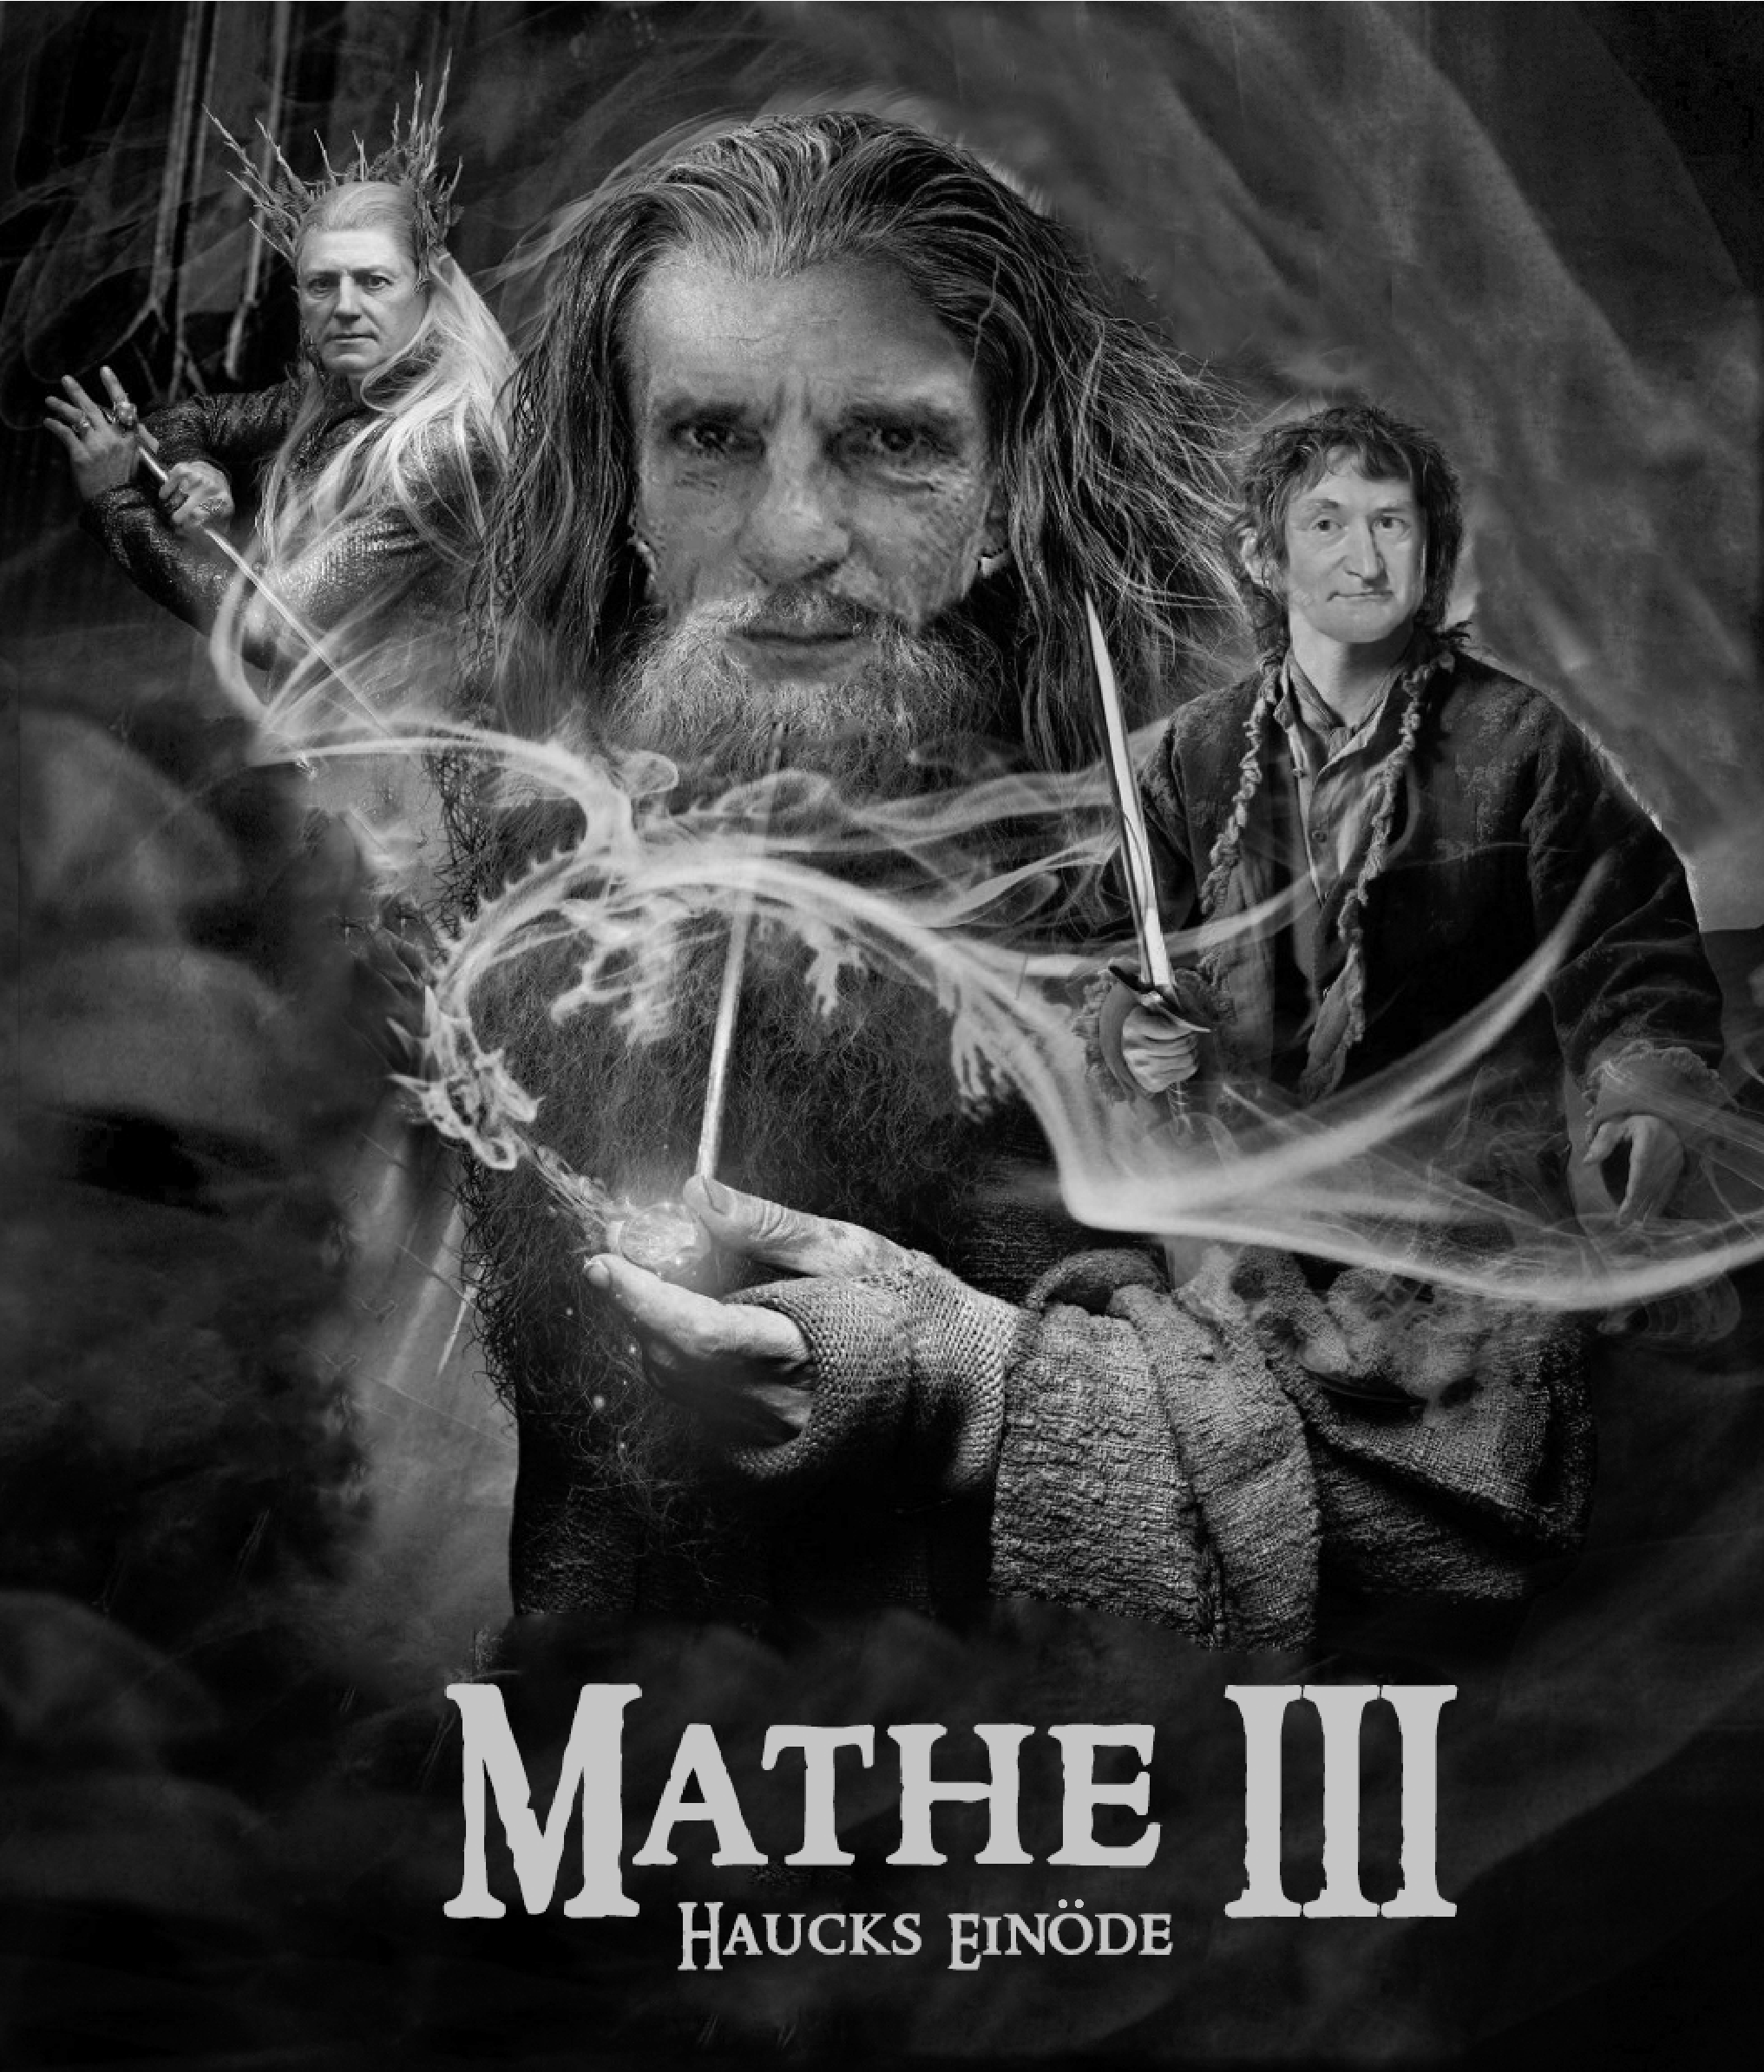
\includepdf{HauksEinoede.pdf}
\author{Finn Ickler nach Peter Hauck\\ Cover by DOS}
\title{Mathe III Skript WS15/16}
\date{13.10.2015-12.2.2016}
\maketitle
\vfill
\thanks{Danke an: Dominik Spoerle, Flavia Nährlich, Lea Buchweitz, Justin Humm, Fabian Mikulasch u.v.a}
\resetHeadWidth
\newpage
\tableofcontents
\listoffigures
\clearpage
\setcounter{section}{-1}
\begin{center}
\Huge Ende des SS 2015
\end{center}
\section{Der Vektorraum $\R^n$}\index{Vektorraum}
$n \in \N\quad \R^n = \left\{ \begin{pmatrix}
a_1\\
\vdots\\
a_n
\end{pmatrix} : a_1 \in \R \right\}$\\
\emph{Spaltenvektoren}\index{Spaltenvektoren} der Länge $n:\: \begin{pmatrix}
a_1\\\vdots\\a_n
\end{pmatrix} = (a_1,\ldots,a_n)^t\\
a_1,\ldots,a_n$ \emph{Komponente}\index{Komponente} der Spaltenvektoren.\\
Wie bei Matrizen:\\
\begin{minipage}{.5\textwidth}\[ \begin{pmatrix}
a_1\\\vdots\\a_n
\end{pmatrix}+ \begin{pmatrix}
b_1\\\vdots\\b_n
\end{pmatrix} = \begin{pmatrix}
a_1 + b_1\\\vdots\\a_n + b_n
\end{pmatrix}\]
\end{minipage}%
\begin{minipage}{.5\textwidth}
(Multiplikation entspricht der Matrizenmultiplikation\index{Matrizenmultiplikation} und ist nicht möglich falls $n > 1$)
\end{minipage}\\
Multiplikation eines Spaltenvektors mit einer Zahl (\emph{Skalar})
\[ a \cd \begin{pmatrix}
a_1\\\vdots\\a_n
\end{pmatrix} = \begin{pmatrix}
aa_1\\\vdots\\aa_n
\end{pmatrix} \]
Addition+Abbildung : $\R^n \times \R^n \to \R^n$\\
$\R^n$ mit Addition und Multiplikation mit Skalaren : \emph{$\R$-Vektorraum}\\
Die Vektoren im $\R^1 (= \R),\R^2$ und $\R^3$ entsprechen Punkten auf der \index{Zahlengerade}Zahlengerade, Ebene, dreidimensionalen Raums.
\begin{figure}[h!]
\centering
\caption{Ein \index{Vektor}Vektor dargestellt durch seinen Ortsvektor}
\begin{tikzpicture}
\begin{axis}[axis equal, axis y line = center, axis x line = center, xmax = 3 , ymax = 3, ymin = 0 , xmin = -0.5,xtick={0.1,2},ytick={2},xticklabels={$\begin{pmatrix}
0\\0
\end{pmatrix}$,$a_1$},yticklabels={$a_2$}]
\draw[->] (axis cs:0,0)--(axis cs: 2,2);
\end{axis}
\end{tikzpicture}
\end{figure}
Punkte des $\R^2,\R^3$ lassen sich identifizieren mit, {\em Ortsvektoren}\index{Ortsvektoren} Pfeile mit Beginn in 0 (Komp = 0) und Ende im entsprechenden Punkt\\
Addition von Spaltenvektoren entspricht der Addition von Ortsvektoren entsprechend der \index{Parallelogrammregel}Parallelogrammregel.
\begin{figure}[h!]
\centering
\caption{Vektoraddition durch Parallelogrammbildung}
\begin{tikzpicture}
\begin{axis}[
axis x line=center,
axis y line=center,
axis equal,
ymin = -1,
xmin = -3,
ymax = 7,
xmax = 5.5,
xtick ={4},
xticklabels={a},
ytick ={1},
yticklabels={b}]
\addplot [black, mark = *, nodes near coords=,every node near coord/.style={anchor=180}] coordinates {( 4, 3)};
   \draw[->](axis cs:0,0)--(axis cs:3.88,2.88);
       \addplot [black, mark = *, nodes near coords=,every node near coord/.style={anchor=0}] coordinates {( -1, 1)};
              \draw[->](axis cs:0,0)--(axis cs:-0.88,0.88);
\addplot [black, mark = *, nodes near coords=,every node near coord/.style={anchor=0}] coordinates {( 3, 4)};
\addplot[mark=none, black] coordinates {(-1,1) (3,4)};
\addplot[mark=none, black] coordinates {(3,4) (4,3)};
\draw[-> ,red](axis cs:0,0)--(axis cs:2.95,3.88);
\end{axis}
\end{tikzpicture}\end{figure}
Multiplikation mit Skalaren a :\\ Streckung (falls $\abs{a} > 1$)\\ Stauchung (falls $0 \ge \abs{a} \ge 1$)\\
Richtungspunkt, falls $a < 0$
%TODO: Steckung und Stauchung\\
\subsection{Satz (Rechenregeln in $\R^n$)}\label{sec:0.1}
Seien $u,v,w \in \R^n,a,b\in\R$ Dann gilt:\\
\begin{enumerate}[a)]
\item \begin{align}
u + (v + w) &= (u + v) + w \tag{1.1}\\
v + 0 = 0 + v &= v, \text{wobei } 0\ \textit{Nullvektor} \tag{1.2}\\
v + -v &= 0 \tag{1.3}\marginnote{$\R^n$ kommutative Gruppe}\\
u + v &= v + u \tag{1.4}\\
(a + b)v &= av + bv \tag{2.1}\\
a(u + v) &= au + av \tag{2.2}\\
(a \cd b)v &=a(bv)\tag{2.3}\\
1v &= v \tag{2.4}
\end{align}
\item $0 \cdot v = 0$ und $ a \cdot 0 = 0$\\
Beweis folgt aus entsprechenden Rechenregeln in 0
\end{enumerate}
\subsection{Definition}\label{sec:0.2}
Eine nicht-leere Teilmenge $\mathcal{U} \supset \R^n$ hei\ss t \emph{Unterraum} (oder \emph{Teilraum} von $\R^n$), falls gilt:
\begin{enumerate}[(1)]
\item $\forall u_1,\,u_2 \in \mathcal{U}:\: u_1 + u_2 \in \mathcal{U}$ (Abgeschlossenheit bezüglich +)
\item $\forall u \in \mathcal{U} \forall a \in \R:\: au \in \mathcal{U}
$(Abgeschlossenheit bezüglich Mult. mit Skalaren)
\end{enumerate}
$\mathcal{U}$ enthält Nullvektor \{0\} Unterraum\index{Unterraum} von $\R^n$ (Nullraum)\index{Nullraum}\\
$\R^n $ ist Unterraum von $\R$
\subsection{Beispiele}\label{sec:0.3}
\begin{enumerate}[a)]
\item $0 \ne v \in \R^2\quad G = \{ av: a \in \R \}$ ist Unterraum von $\R^n$\\\begin{minipage}{.3\textwidth}
($a_1v,a_2v \in G, (a_1 + a_2)v \in G$\quad2.1 in \ref{sec:0.2}\\
$av \in G, b \in \R (ba)v \in G$)
\end{minipage}\\
G = Ursprungsgerade durch $\begin{pmatrix}
0\\0
\end{pmatrix}$ und v = $\begin{pmatrix}
a_1\\a_2
\end{pmatrix}
n = 2$:
\begin{figure}[h!]
\centering
\caption{Gerade dargestellt durch Vektoren}
\begin{tikzpicture}
\begin{axis}[axis equal, axis y line = center, axis x line = center, xmax = 3 , ymax = 2, ymin = -2, xmin = -0.5,xtick={0.1,2},ytick={2},xticklabels={$\begin{pmatrix}
0\\0
\end{pmatrix}$,$a_1$},yticklabels={$a_2$}]
\draw[blue,thick] (axis cs:-2,-2)--(axis cs: 2,2);
\end{axis}
\end{tikzpicture}
\end{figure}
\item $v,w \in \R^n\\
E = \{ av + bw : a,b \in \R \}$ ist Unterraum von $\R^n\\
v = o, w = o :\: E = \{ o \}\\
v \ne o\quad w \not\in \{ av:\: a \in \R \}\\
E = \R^2 $
$n = 3:\:$ Ebene durch $\begin{pmatrix}
0\\0\\0
\end{pmatrix}$ und durch $v,w$\\
Ist $w \in \{ av : a \in \R \},$ so ist $E = G$ (aus a))
\item $v,w \ne o\\
G' = \{ w + av : a \in \R\}$\\
$[v \in G' \Leftrightarrow \exists a \in \R: w+ av \in o \Leftrightarrow \exists a \in \R :\: w = (-a)v \in G]$
\end{enumerate}
\subsection{Satz}\label{sec:0.4}
Seien $\mathcal{U}_1,\mathcal{U}_2$ Unterräume von $\R^n$
\begin{enumerate}[a)]
\item $\mathcal{U}_1 \cap \mathcal{U}_2$ ist Unterraum von $\R^n$
\item $\mathcal{U}_1 \cup \mathcal{U}_2$ ist im Allgemeinen \textsc{kein} Unterraum von $\R^n$
\item $\mathcal{U}_1 + \mathcal{U}_2 := \{u_1 + u_2 : u_1:\: \mathcal{U}_1, u_2:\: \mathcal{U}_2\}$
(Summe von $\mathcal{U}_1$ und $\mathcal{U}_2$) ist Unterraum von $\R^n$.
\item $\U_1 \subseteq \U_1 + \U_2$\quad$\U_2 \subseteq \U_1+\U_2$ und $\U_1 + \U_2$ ist der kleinste Unterraum von $\R^n$, der $\U_1$ und $\U_2$ enthält. (d.h ist $w$ Unterraum von $\R^n$ mit $\U_1,\U_2 \in w,$ so $\U_1 + \U_2 \subseteq W$)
\end{enumerate}
\begin{proof}
a) $\checkmark$\\
b) %TODO\\
c) %TODO
\end{proof}
\subsection{Beispiel}\label{sec:0.5}
\begin{enumerate}[a)]
\item \ref{sec:10.3}b)
$G_1 = \{ av :\: a \in \R \}\\
G_2 = \{ aw :\: a \}\\
G_1 + G_2 = E$
\item $\R^3\\
E_1 = \left\{ r \cd \begin{pmatrix}
1\\0\\0
\end{pmatrix} + s \cd \begin{pmatrix}
0\\0\\1
\end{pmatrix}:\: r,s\in\R \right\}\\
\phantom{E_1} = \left\{\begin{pmatrix}
r\\0\\s
\end{pmatrix}:\: r,s\in\R \right\}\\
E_2= \left\{ t \cd \begin{pmatrix}
0\\1\\0
\end{pmatrix} + u \cd \begin{pmatrix}
1\\1\\1
\end{pmatrix} \right\}\\
\phantom{E_2}= \left\{\begin{pmatrix}
u\\t+u\\u
\end{pmatrix} \right\}$\\
$E_1 + E_2$ Unterräume von $\R^3$ (10.3.b)\\
$E_1 \cap E_2 = ?\\
v \in E_1 \cap E_2 \Leftrightarrow v = \begin{pmatrix}
r\\0\\s
\end{pmatrix} = \begin{pmatrix}
u\\t+u\\u
\end{pmatrix} \Leftrightarrow r = u, t + u = 0 , s = u\\
E_1 \cap E_2 = \left\{ \begin{pmatrix}
u\\0\\u 
\end{pmatrix}: u \in \R\right\}\\
\phantom{E_1 \cap E_2} = \left\{ u \cd \begin{pmatrix}
1\\0\\1
\end{pmatrix}: u \in \R \right\}\\
E_1 + E_2 = ?\\
E_1 + E_2 = \R^3$, denn :\\
Es gilt sogar:\\
$\R^3 = E_1 + G_2$, wobei\\
$G_2 = \left\{ t \cd \begin{pmatrix}
0\\1\\0
\end{pmatrix}: t \in \R \right\} \subseteq E_@\\
\begin{pmatrix}
x\\y\\z
\end{pmatrix} = x \cd \begin{pmatrix}
1\\0\\1
\end{pmatrix} z\cd \begin{pmatrix}
0\\0\\1
\end{pmatrix} + y \cd \begin{pmatrix}
0\\1\\0
\end{pmatrix} = \begin{pmatrix}
x\\0\\z
\end{pmatrix} + \begin{pmatrix}
0\\y\\0
\end{pmatrix}\\
\begin{pmatrix}
x\\y\\z
\end{pmatrix} =  (x-y) \begin{pmatrix}
1\\0\\0
\end{pmatrix} + (z-y)\begin{pmatrix}
0\\0\\1
\end{pmatrix} + y \begin{pmatrix}
1\\1\\1
\end{pmatrix}$\\
$\phantom{\begin{pmatrix}
0\\0\\1
\end{pmatrix}}=\begin{pmatrix}
x-y\\0\\z-y
\end{pmatrix} + \begin{pmatrix}
y\\y\\y
\end{pmatrix}$
\end{enumerate}
\subsection{Definition}\label{sec:0.6}
\begin{enumerate}[a)]
\item$v_1,\ldots , v_m \in \R^n, a_1,\ldots a_m \in \R$\\
Dann hei\ss t $a_1v_1 + \ldots + a_m v_m = \sum_{i = 1}^{m} a_iv_i\\
$\emph{Linearkombination}\index{Linearkombination} von $v_1,\ldots ,v_m$ (mit Koeffizienten $a_1,\ldots,a_m$).\\
$[ $Zwei formal verschiedene Linearkombinationen der gleichen $v_1,\ldots, v_m$ können den gleichen Vektor darstellen \\
$1 \cd \begin{pmatrix}
1\\0
\end{pmatrix} + 2 \cd \begin{pmatrix}
0\\1
\end{pmatrix} + 3 \cd \begin{pmatrix}
1\\1
\end{pmatrix} = 2 \cd \begin{pmatrix}
1\\0
\end{pmatrix} + 3 \cd \begin{pmatrix}
0\\1
\end{pmatrix} + 2 \cd \begin{pmatrix}
1\\1
\end{pmatrix} = \begin{pmatrix}
4\\5
\end{pmatrix}]$
\item Ist $M \subseteq R^n$, so ist der von M \emph{erzeugte} (oder \emph{aufgespannte}) Unterraum $\langle M \rangle_\R$ (oder $\langle M \rangle$) die Menge aller (endlichen) Linearkombinationen, die man mit Vektoren aus M bilden kann.\\
$\langle M \rangle_\R = \left\{ \sum\limits_{i=1}^{n}a_iv_i : n\in\N , a_i \in\R ,v_i\in M \right\}$ falls $M \ne \varnothing\\
\langle\varnothing\rangle_\R := \{ \varnothing \}\\
M = \{ v_1,\ldots v_m \}$, so %TODO...
\end{enumerate}
\subsection{Beispiel}\label{sec:10.7}
\begin{enumerate}[a)]
\item $e_i = \begin{pmatrix}
0\\0\\1\\0\\0
\end{pmatrix}\in\R^n\\
\langle e_1,\ldots e_n\rangle = \R^n\\
\begin{pmatrix}
x_1\\\vdots\\x_n
\end{pmatrix} = x_1e_1+x_2e_2+\ldots+x_ne_n$
\item $\U = \langle \begin{pmatrix}
1\\2\\3
\end{pmatrix},\begin{pmatrix}
3\\2\\1
\end{pmatrix},\begin{pmatrix}
2\\3\\4
\end{pmatrix}\rangle_\R$\\
Ist $\U = \R^3$?\\
Für welche $\vektor{x}{y}{z} \in \R^3$ gibt es geeignete Skalare $a,b,c\in\R$ mit $a\vektor{1}{2}{3}+b\vektor{3}{2}{1}+c\vektor{2}{3}{4}?\\$
\[ \begin{matrix}
a &+3b&+2c&=x\\
2a&+2b&+3c&=y\\
3a&+b &+4c&=z
\end{matrix} \]
LGS für die Unbekannten $a,b,c$ mit variabler rechter Seite : Gau\ss\\
\[ \begin{pmatrix}
1&3&2&&x\\
2&2&3&&y\\
3&1&4&&z
\end{pmatrix}\quad\to\quad\begin{pmatrix}
1&3&2&&x\\
2&-4&-1&&y-2x\\
0&-8&-2&&z-3x
\end{pmatrix}   \]\\
\[\to\quad\begin{pmatrix}
1&3&2&&x\\
0&1&\frac14&&\frac{2x-y}4\\
0&0&0&&x-2y+z
\end{pmatrix} \]
LGS ist lösbar $\Leftrightarrow x-2y+z=0$.\\
Dass hei\ss t $\vektor{x}{y}{z} \in \U \Leftrightarrow x -2y = z =0\\
\U = \left\{ \vektor{x}{y}{z} : x-2y+z=0,x,y,z\in\R \right\}\\
\phantom{\U}= \left\{ \vektor{x}{y}{-x+2y} : x,y\in\R \right\}\\
\vektor{2}{3}{4}\in\U$
\end{enumerate}
Lösungen des LGS: $c$ frei wählen, b, a ergeben sich, (falls $x-2y + z = 0)$ z.B $c = 0, b = \frac12x-\frac14y, a = x-3b = -\frac12x + \frac34y$\\
Ist $\mathit{x-2y+z=0}$, so ist\\ $\vektor{x}{y}{z} = (-\frac12x+\frac34y)\vektor{x}{y}{z}+ (\frac12x - \frac14y)\vektor{3}{2}{1}\\
\vektor{2}{3}{4}\frac54\vektor123+\frac14\vektor321\\
\U= \left\langle\vektor123, \vektor321 \right\rangle_\R$
\[\cancel{\begin{matrix}
6x^2&- 3xy&+y^3 &=5\\
7x^3&+ 3x^2y^2&-xy&=7
\end{matrix}} \]
\setcounter{subsection}{8}
\subsection{Definition}\label{sec:0.9}
$v_1,\ldots,v_n \in \R^n$ hei\ss en \emph{linear abhängig}. falls
$a_1,\ldots,a_n \in \R$ existieren, \emph{nicht alle = 0}, mit $a_1v_1 + \ldots +a_nv_n = 0$.\\
Gibt es solche Skalare nicht, so heißen $v_1,\ldots,v_m$ \emph{linear unabhängig} (d.h. aus $a_1v_1\ldots a_nv_n = 0 folgt a_1 = \ldots = a_n = 0$).\\
(Entsprechend $\{ v_1\ldots v_n \}$ linear abhängig/linear unabhängig)\\
Per Definition : $\varnothing$ is linear unabhängig.\\
\subsection{Beispiel}\label{sec:0.10}
\begin{enumerate}[a)]
\item $\sigma$ + v $\in \R^n$ Dann ist v linear unabhängig:\\
Zu zeigen : Ist av = $\sigma \Rightarrow a = 0$\\
Sei $v \vektor{b_1}{\vdots}{b_n}$ Da $v\ne \sigma$,\\
existiert mindestens ein i mit $b_i \ne 0$.\\
Angenommen $\sigma v = \vektor{0 b_1}{\vdots}{0 b_n} = \vektor000 = \sigma $. \\
Dann $ab_i = 0$ Da $b_i \ne 0$, folgt a = 0.\\
$\sigma$ ist linear abhängig: \[1 \cd \sigma = \sigma \]
\item $v_1 = \sigma .v_2\ldots,v_m$ ist linear abhängig :\\
$\sigma = 1 \cd \sigma + 0 \cd v_2 + \ldots + 0 \cd v_m$
\item $v,w \in \R^n\\
v \ne \sigma \ne w$\\
\textcircled{\raisebox{-1pt}{1}}\parbox{.2\textwidth}{v,w sind linear abhängig} $\Leftrightarrow\\
\textcircled{\raisebox{-1pt}{2}} v \in \langle w \rangle_\R \Leftrightarrow\\
\textcircled{\raisebox{-1pt}{3}} w \in \langle v \rangle_\R \Leftrightarrow\\
\textcircled{\raisebox{-1pt}{4}} \langle v \rangle_\R = \langle w \rangle_\R$\\
\textcircled{\raisebox{-1pt}{1}}\\
$v,w$ linear abhängig $\rightarrow \exists a_1,a_2\in \R,$ nicht beide = 0, $a_1v + a_2w = \sigma$. Dann beide $(a_1,a_2) \ne 0\\
a_1v = -a_2w \mid \cd \frac1{a_1}\\
v = - \frac{-a_2}{-a_1}w \in \langle w \rangle_\R  \textcircled{\raisebox{-1pt}{2}}\\
\textcircled{\raisebox{-1pt}{2}}\\
v \in \langle w \rangle_\R$ dass hei\ss t $v = aw$ für ein $a \in \R$ Dann $a \ne 0$, da $v \ne \sigma$. $w = \frac1a \cd v \in \langle v \rangle_\R \textcircled{\raisebox{-1pt}{3}}$\\
\textcircled{\raisebox{-1pt}{3}}\\
$w = bv$ für ein $b \in \R b \ne 0$,da $w \ne \sigma.\\
aw \in \langle w \rangle_\R \Rightarrow aW = (ab)v \in \langle v\rangle_\R\\
\langle w \rangle_\R \subseteq \langle v \rangle_\R$\\
$w = \frac1b w$ Dann analog $\langle v \rangle\R \subseteq \langle w \rangle_\R$\\
Also $ \langle v \rangle\R = \langle w \rangle_\R$\textcircled{\raisebox{-1pt}{4}}\\
\textcircled{\raisebox{-1pt}{4}}\\
$v \in \langle v \rangle_\R = \langle w \rangle_\R$, dass hei\ss t.\\
$ v = a \cd w$ für ein $a \in \R\\
a \cd v + (-a) w = \sigma \Rightarrow v,w$ sind linear abhängig \textcircled{\raisebox{-1pt}{1}}
\item $e_i = \begin{pmatrix}
0\\\vdots\\0\\1\\0\\0\\0
\end{pmatrix} \in \R^n\\
e_1,\ldots,e_n$ sind linear unabhängig.\\
$\sigma = a_1e_1 + \ldots a_ne_n = \begin{pmatrix}
0\\\vdots\\0\\1\\0\\0\\0
\end{pmatrix} + \begin{pmatrix}
0\\\vdots\\0\\a_2\\0\\0\\0
\end{pmatrix} \Rightarrow a_1 = a_2 = \ldots = a_n = 0$
\item $\vektor12{},\vektor{-3}1{},\vektor62{}$ sind linear abhängig $\R^2$: \\
Gesucht sind alle $a_i,b_i \in \R$ mit $a \cd \vektor12{} + b \cd \vektor{-3}1{} + c \cd \vektor62{} = \vektor00{}$\\
Führt auf LGS für a,b,c:\\
$\begin{pmatrix}
1&-3&6&&0\\
2&1&2&&0
\end{pmatrix}\quad\rightarrow\quad \begin{pmatrix}
1&-3&6&&0\\
0&7&-10&&0
\end{pmatrix}\\
c$ ist frei wählbar
\item $\vektor123, \vektor321, \vektor234$ sind linear abhängig in $\R^3$,\\
10.8b) : $\frac54 \vektor123 + \frac14 \vektor321 + (-1)\vektor234 = \vektor000$
\end{enumerate}
\subsection{Satz}\label{sec:0.11}
Seien $v_1,\ldots,v_n \in \R^n$
\begin{enumerate}[a)]
\item $v_1,\ldots,v_m$ sind linear abhängig \textcircled{\raisebox{-1pt}{1}}\\
$\Leftrightarrow \exists i \ldots v_i = \sum\limits^{m}_{\substack{j=1\\j\ne i} }b_jv_j \textcircled{\raisebox{-1pt}{2}} \\\Leftrightarrow \exists i : \langle v_1,\ldots,v_m \rangle_\R = \langle v_1, \ldots v_{i-1}, v_{i+!},\ldots,v_m\rangle_\R$\textcircled{\raisebox{-1pt}{3}}
\item $v_1,\ldots,v_m$ sind linear unabhängig $\Leftrightarrow$ Jedes $v \in \langle v_1,\ldots,v_m\rangle_\R$ lässt sich auf \emph{genau eine} Weise als Linearkombination von $v_1,\ldots,v_m$ schreiben.
\item Sind $v_1,\ldots,v_m$ linear unabhängig und es existiert $v \in \R^n$ mit$ v \ne \langle v_1,\ldots,v_m\rangle_\R$ dann sind auch $v_1,\ldots,v_m,v $ linear unabhängig
\end{enumerate}
\begin{proof}
a) \textcircled{\raisebox{-1pt}{1}} $\Rightarrow$ \textcircled{\raisebox{-1pt}{2}}\\
$v_1,\ldots v_m$ sind linear abhängig\\
$\Rightarrow \exists a_1,\ldots,a_m$ nicht alle = 0,\\
$a_av_i + \ldots + a_mv_m = 0$\\
Sei $a_i \ne 0\\
a_iv_i = \sum\limits_{\substack{j =1\\j\ne i}}^{m} -a_jv_j$\\
$\phantom{a_i}v_i = \sum\limits_{\substack{j =1\\j\ne i}}^{m} -\frac{a_j}{a_i}v_j$ \textcircled{\raisebox{-1pt}{2}}\\
\textcircled{\raisebox{-1pt}{2}} $\Rightarrow \textcircled{\raisebox{-1pt}{3}}$\\
Klar : $\langle v_1,\ldots v_{i-1},v_{i+1},v_m \rangle_\R \subseteq \langle v_1, \ldots ,v_m \rangle_\R$\\
Zeige $\supseteq$\quad $v  = \langle v_1,\ldots, v_m \rangle_\R$, d.h\\
$v = \sum\limits_{j=1}^{m} a_jv_j = \sum\limits_{\substack{j=1\\j\ne i}}^{m} a_jv_j + a_i (\sum\limits_{\substack{j=1\\j\ne i}}^{m} b_jv_j) = \sum\limits_{\substack{j=1\\j\ne i}}^{m} (a_j + a_i b_j)v_j \in \langle v_1,\ldots v_{i-1},v_{i+1}.\ldots,v_m \rangle_\R \textcircled{\raisebox{-1pt}{2}}$
\textcircled{\raisebox{-1pt}{3}} $ \Rightarrow \textcircled{\raisebox{-1pt}{1}}\\
v_i \in \langle v_1 \ldots v_m \rangle_\R = \langle v_1 \ldots v_{i-1}, v_{i+1}, \rangle_\R$, dass hei\ss t es existiert \\
$a_1, \ldots a_{i-1},a_{i+1},\ldots a_{m} \in \R$ mit \[ v_i = \sum_{\substack{j=1\\j \ne i}}^{m} a_jv_j \]
$\Rightarrow \sigma = a_1 + v_1 + \ldots + a_{i-1}v_{i-1} + (-1)v_i + a_{i+1}v_{i+1} + \ldots a_mv_m \qquad v_1\ldots v_m $ linear abhängig 
%TODO Beweis b und c
\end{proof}
\subsection{Satz}\label{sec:0.12}
Sind $v_i, \ldots, v_{n+1} \in \R^n$, so\\
sin $v_i,\ldots, v_{n+1}$ linear abhängig.\\
(Insbesondere ist $m > n$ und $v_i,v_m \in \R^n$, so sind $v_1,\ldots,v_m $ linear abhängig)
\begin {proof}
Suche alle $a_1,\ldots,a{n+1} \in \R$ mit $a_iv_1 + \ldots a_{n+1}v_{n+1} = \vektor0\dots0$\\
Führt zu LGS für $a_1,\ldots, a_{n+1}$ mit Koeffizientenmatrix $(v_1,\ldots, v_2, \ldots, v_{n+1}) =A$\\
Frage : Hat $ A \cd \vektor{a_i}\vdots{a_{n+1}} = \vektor0\vdots0 \in \R^n$ nicht triviale Lösung?\\
Gau\ss\ :\\
$\left(\raisebox{-0.5cm}{\scalebox{4}{A}} \vektor0\vdots0 \longrightarrow \right)$
%TODO Rest von 10.12
\end {proof}
\subsection{Definition}\label{sec:0.13}
Sei $\U$ ein Unterraum von $\R^n$\\
$B \subseteq \U$ hei\ss t Basis von $\U$ falls:
\begin{enumerate}[(1)]
\item $\langle B \rangle_\R = U$
\item B ist linear unabhängig 
\end{enumerate}
($\U = \{\sigma\}, B = \varnothing$)
\subsection{Beispiel}\label{sec:0.14}
\begin{enumerate}[a)]
\item $e_1,\ldots,e_n$ ist Basis von $\R^n$ (kanonische Basis)\\
$e_1 = \begin{pmatrix}
0\\\vdots\\1\\0\\0
\end{pmatrix}\leftarrow i\\
\vektor{a_i}\vdots{a_n} = \sum_{i=1}^{n} a_ie_i$
\item $\vektor12{},\vektor32{}$ ist Basis von $R^2$:\\
Sei $\vektor{x}{y}{}\in R^2$. Gesucht: $a,b \in \R$ mit $a\vektor12{}+b\vektor32{} =\vektor{x}{y}{}$\\
LGS mit variabler rechter Seite\[
\begin{matrix}
1a &+3b&=x\\
2a &+2b&=y
\end{matrix}\]
Gau\ss:\medskip\\
$\begin{pmatrix}
1&3&&x\\
2&2&&y
\end{pmatrix}\quad\rightarrow\quad\begin{pmatrix}
1&3&&x\\
0&-4&&y-2x
\end{pmatrix}$\\
Eindeutige Lösung: $b = -\frac14y+\frac12x\quad a = x-3b = x +\frac34y - \frac32x = -\frac12x + \frac34y$\\
z.B $\vektor{x}{y}{} = \vektor10{}\\
\vektor10{} = -\frac12\vektor12{}+ \frac12\vektor32{}
\R^2 \langle \vektor12{},\vektor32{}\rangle\\
\vektor12{},\vektor32{}$ sind linear unabhängig nach \ref{sec:0.10}c)\\
$\left\{\vektor12{},\vektor32{}\right\}$ Basis.
\item $\U = \left\langle \vektor123,\vektor321,\vektor234\right\rangle_\R\\
\vektor234 = \frac54 \vektor123 + \frac14\vektor321\\
\U = \left\langle \vektor123,\vektor321\right\rangle_\R\\
\vektor123,\vektor321$ linear unabhängig (\ref{sec:0.10}c))\\
$\left\{ \vektor123, \vektor321 \right\}$ Basis von $\U$
\end{enumerate}
\subsection{Satz}\label{sec:0.15}
Jeder Unterraum $\U$ des $\R^n$ besitzt eine Basis.
\begin{proof}
Ist $\U = \{\sigma\}$,so $b = \varnothing$.\\
Sei also $\U \ne \{\sigma\}$.\\
$v_1$ ist linear unabhängig.\\
$\langle v_1\rangle_\R \subseteq \U.$\\
Ist $\U = \langle v_1 \rangle_\R$, so ist $\{ v_1 \}$ Basis von $\U$\\
Ist $\langle v_1 \rangle_\R \subsetneq \U$.\\
Sei $v_2 \in \U \setminus \langle v_1 \rangle_\R$.\\
Nach \ref{sec:0.11}c) ist $\{ v_1,v_2 \}$ linear unabhängig. Ist $\rangle v_1,v_2 \rangle = \U$, so ist $\{ v_1.v_2 \}$ Basis von $\U$.\\
Ist $\langle v_1, v_2 \rangle_\R \subsetneq U$ so wähle $v_3$ usw.\\
Es existiert $m \ne n$ mit $\langle v_1,\ldots v_m\rangle_\R = \U$ und $v_1\ldots,v_m$ sind linear unabhängig.\\
(Denn noch \ref{sec:0.12} gibt es im $\R^n$ keine n+1 linear unabhängige Vektoren)
\end{proof}
\subsection{Satz}\label{sec:0.16}
Je zwei Basen $B_1,B_2$ eines Unterraums $\U$ des $\R^n$ enthalten die gleiche Anzahl von Vektoren $\abs{B_1} = \abs{B_2}$.\\
Insbesondere:\\
Je zwei Basen des $\R^n$ enthalten n Vektoren
\subsection{Definition}\label{sec:0.17}
Ist $\U$ Unterraum von $\R^n$, B Basis von $\U,\, \abs{B} = m$.\\
Dann ist $m$ die \emph{Dimension} von $\U$, $\dim(u) = m.$\\
$\dim(\R^n) = n,\, \dim(\U) \ne n$.
\subsection{Satz (Basisergänzungssatz)}\label{sec:0.18}
Sei $\U$ Unterraum der $\R^n, M \subseteq \U$ eine Menge m linear unabhängiger Vektoren. Dann lässt sich M zu einer Basis von $\U$ ergänzen.
\begin{proof}
Analog zu \ref{sec:0.15}
\end{proof}
\subsection{Korollar}
Ist $\U$ Unterraum des $\R^n$ und $\dim(\U) = n$, dann ist $\U = \R^n$
\begin{proof}
Sei B Basis von $\U$, also $\abs{B} = n$.\\
Nach \ref{sec:0.18} (dort mit $\U = \R^n, M = B$) lässt sich B zu Basis B' von $\R^n$ ergänzen.\\
$\dim(\R^n) = n \Rightarrow \abs{B'} = n.$\\
Also B = B'\\
$\R^n = \langle B'\rangle_\R = \langle B \rangle_\R = \U$
\end{proof}
\subsection{Definition}
Ist $\U$ Unterraum von $\R^n$, B = ($u_1\ldots,u_m$) eine geordnete Basis von $\U$. Nach \ref{sec:0.11}b), lässt sich jeder Vektorraum $\U = \langle B\rangle_\R$ \emph{eindeutig} als Linearkombination \[ \U = \sum_{i=1}^{m} a_iu_i\quad,a_i \in \R \] schreiben.\\
$(a_1\ldots,a_m)$ hei\ss en \emph{Koordinaten} von u bzgl. der Basis B.
\subsection{Beispiele}
\begin{enumerate}[a)]
\item B($e_1\ldots,e_m$) kanonische Basis von $\R^n$.\\
Koordinaten von $\vektor{a_1}\vdots{a_n} \in \R^n$ bzgl. B:\\
$(a_1\ldots,a_n)$ \emph{kartesische} Koordinaten. \hfill (\emph{Rene Descartes, 1596-1650}) 
\end{enumerate}
\newpage
\begin{center}
\Huge Anfang des WS 2015/16
\end{center}\section{Algebraische Strukturen}
\marginpar{13.10.2015}
\subsection{Definition}\label{sec:1.1}
Sei $X \neq \varnothing$. Eine \index{Verknüpfung}\emph{Verknüpfung} auf $X$ ist \index{Abbildung}: \\ $\begin{cases}
X \times X &\longrightarrow X\\
(a,b) &\longrightarrow a \star b
\end{cases}$ ('Produkt' von a und b)\\
$\star$ ist Platzhalter für andere \index{Verknüpfungssymbole}Verknüpfungssymbole, die in speziellen Beispielen auftreten können.
\subsection{Beispiele}\label{sec:1.2}
\begin{enumerate}[a)]
\item Addition $+$ und Multiplikation $\cd$ sind Verknüpfungen auf $\N, \Z, \mathbb{Q}, \R, \mathbb{C}$.
Multiplikation ist \emph{keine} Verknüpfung auf der Menge der negativen ganzen Zahlen.
\item Division ist keine Verknüpfung auf $\N$. Division ist Verknüpfung auf $\mathbb{Q} \setminus \{0\}, \R \setminus \{0\}, \C \setminus \{0\}$
\item $\Z_n : = \{ 0,1,\ldots,n-1 \}$ \hfill $(n \in \N)\\
a \oplus b : = (a + b) \mod n \in \Z_n\\
a \circledcirc b := (a \cd b) \mod n \in \Z_n$\\
Verknüpfungen auf $\Z_n\\
n = 7:\qquad 5 \circledcirc 6 = 2\\
\phantom{n = 7::}\qquad 5 \oplus 6 = 4\\
n = 2:\qquad \Z_n = \{0,1\}\\
\phantom{n = 2::}\qquad0 \oplus 0 = 0, 1 \oplus 0 = 1,0 \oplus 1 = 1, 1 \oplus 1 = 0\\
\phantom{n = 2::}\qquad\circledcirc = \cdot$
\item M Menge, X = Menge aller Abbildungen $M \longrightarrow M$. Verknüpfung auf X: Hintereinanderausführung von Abbildungen: $\circ$\\
$(f, g): M \longrightarrow M$, So $f\circ g:\:M \to M\\
(f \circ g)(m) = f(g(m)) \in M, m \in M$\\
Im Allgemeinen ist $g \circ f \ne f \circ g$
\item $X = \{0,1\}$\\
2-stellige Aussagen, Junktoren wie $\land,\lor,$\textsf{ XOR }$,\Rightarrow,\Leftrightarrow$ hei\ss en Verknüpfungen auf $X$.
0 entspricht f, 1 entspricht w.\\
$0 \lor 0 = 0, 1 \lor 0 = 1, 0 \lor 1 = 1, 1 \lor 1 = 1\\
0 \land 0 = 0, 0 \land 1 = 0, 1 \land 0 = 0, 1 \land 1 =1$ (= 'Multiplikation')\\
$0 \textsf{ XOR } 0 = 0, 1 \textsf{ XOR } 0 = 1, 0 \textsf{ XOR } 1 = 1, 1 \textsf{ XOR } 1 = 0$ (= Addition mod 2)
\item $X = M_n(\R)$ = Menge der  $n \times n$- Matrizen über $\R$.\\ \index{Matrizenaddition}Matrizenaddition ist Verknüpfung auf $X$.\\
\index{Matrizenmultiplikation}Matrizenmultiplikation ist Verknüpfung auf $X$.
\item $M$ Menge. $X$ Menge aller endlichen Folgen von Elementen aus M ('Wörter' über M).\\
Verknüpfung: Hintereinanderausführung zweier Folgen (\index{Konkatenation}Konkatenation).\\
$M = \{0,1\}, w_1 = 1101, w_2 = 001\\
w_1w_2 = 110111\\
w_2w_1 = 0011101$\\
\end{enumerate}
\subsection{Definition}\label{sec:1.3}
Sei $X \ne 0$ eine Menge mit Verknüpfung $\star$.
\begin{enumerate}[a)]
\item $X$, genauer $(X,\star)$ ist \index{Halbgruppe}\emph{Halbgruppe}, falls
($a \star b) \star c = a \star (b \star c)$ für alle $a,b,c \in X.$ (\index{Assoziativgesetz}\emph{Assoziativgesetz})
\item $(X,\star)$ hei\ss t \index{Monoid}\emph{Monoid}, falls $(X,\star)$ Halbgruppe ist und ein $e \in X$ existiert mit $e \star a = a$ und $a \star e = a$ für alle $a \in X$. e hei\ss t \index{neutrales Element}\emph{neutrales Element} (später, e ist eindeutig bestimmt).
\item Sei $(X,\star)$ ein Monoid. Ein Element $a \in X$ hei\ss t \index{invertierbar}\emph{invertierbar}, falls $b \in X$ existiert (abhängig von a) mit $a \star b = b \star a = e$. b hei\ss t \emph{inverses Element}\index{inverses Element} (das \emph{Inverse}\index{Inverse}) zu a (später: wenn b existiert, so ist es eindeutig bestimmt).
\item Monoid $(X,\star)$ hei\ss t \index{Gruppe}\emph{Gruppe}, falls jedes Element in $X$ bezüglich $\star$ invertierbar ist.
\item Halbgruppe, Monoid, Gruppe $(X,\star)$ bezüglich kommutativ (oder \index{abelsch}\emph{abelsch}) falls $a \star b = b \star a $ für alle $a,b \in X$ (\index{Kommutativgesetz}Kommutativgesetz). \\(Nach: Abel, 1802-1829)
\end{enumerate}
\marginpar{14.10.2015}
\subsection{Bemerkung}\label{sec:1.4}
In Halbgruppe liefert jede sinnvolle Klammerung eines Produktes mit endlich vielen Faktoren das gleiche Element.
\begin{equation}
\tag{n = 4}
(a \star (b \star c)) \star d \underset{\text{AG\footnotemark[1]}}{=} ((a \star b)\star c)\star d \underset{\text{AG\footnotemark[1]}}{=} (a \star b) \star (c \star d) \underset{\text{AG\footnotemark[1]}}{=} a \star (b (c \star d)) \underset{\text{AG\footnotemark}}{=} a \star ((b \star c)\star d)
\end{equation}\footnotetext[1]{Assoziativgesetz}
Klammern werden daher meist weggelassen.\\
$a^n = \underset{\substack{\longleftarrow n \longrightarrow\\
n \in \R}}{a\star\ldots\star a}$ ''Potenzen eindeutig definiert''
\subsection{Proposition}\label{sec:1.5}
\begin{enumerate}[a)]
\item In einem Monoid $(X,\star)$ ist das neutrale Element eindeutig bestimmt.
\item Ist $(X,\star)$ Monoid und ist $a \in X$ invertierbar, so ist das Inverse zu a eindeutig bestimmt. Bezeichnung: $a^{-1}$
\item Ist $(X, \star)$ Monoid und wenn $a,b \in X$ invertierbar sind, so auch $a \star b.\\
(a \star b)^{-1} = b^{-1} \star a^{-1}$
\item Die Menge der invertierbaren Elemente in einem Monoid $(X, \star)$ bilden bezüglich $\star$ eine Gruppe.
\end{enumerate}
\begin{proof}
a) Angenommen: $e_!,e_2$ sind neutrale Elemente. Dann:
\begin{align}
e_1 = e_1 \star e_2 = e_1 \star e_2 = e_2 \qquad{\text{\Lightning}}\notag
\end{align}
b) Angenommen a hat 2 inverse Elemente $b_1, b_2$ also.
\begin{align}
a \star b_1 &= e, b_2 \star a = e \notag\\
b_1 = e \star b_1 = (b_2 \star a) \star b_1 &= b_2 \star (a \star b_1) = b_2 \star e = b_2 \qquad \text{\Lightning} \notag
\end{align}
c) $$(a \star b)\star (b^{-1} \star a^{-1}) = a \star (b \star b^{-1}) \star a^{-1} = a \star e \star a^{-1} = e$$\\
Analog: $(b^{-1} \star a^{-1})\star (a \star b) =e $\\
Also: $(a \star b)^{-1} = b^{-1} \star a^{-1}$\\
d) $\mathcal{I}$= Menge der inversen Elemente in $(X, \star)$,\\ $e \in \mathcal{I}$, dann $e \star e = e,$ dass hei\ss t $e^{-1} = e, \star$ ist Verknüpfung auf $\mathcal{I}$.\\
Zu zeigen: $a,b \in \mathcal{I} \Rightarrow a \star b \in \mathcal{I}$ Folgt aus c).\\
Assozativgesetz gilt in $\mathcal{I}, a \in \mathcal{I} \Rightarrow a^{-1} \in \mathcal{I}$, denn $(a^{-1})^{-1} = a$
\end{proof}
\emph{Bemerkung}: Multiplikation mit $a^{-1}$ macht Multiplikation mit $a$ (Verknüpfung) rückgängig.
\subsection{Beispiel}\label{sec:1.6}
\begin{enumerate}[a)]
\item $\N,\Z,\mathbb{Q},\R,\C$ sind Halbgruppen bezüglich +.\\
$\Z,\mathbb{Q},\R,\C$ sind bezüglich + Monoide mit neutralen Element 0.\\
$\N = \{ 1,2,\ldots \}$ ist kein Monoid bezüglich +, aber $\N_0$.\\
$\Z,\mathbb{Q},\R,\C$ sind Gruppen bezüglich +. Inverses Element zu $a : -a\\
\N$ ist keine Gruppe bezüglich +, Inverse Elemente in $\N_0:\: \{0\}$
\item $\N,\Z,\mathbb{Q},\R,\C$ sind Monoide bezüglich $\cdot$ (neutrales Element 1). Keine Gruppen (in $\Z, \mathbb{Q},\R,\C$ ist 0 nicht invertierbar).\\
$\mathbb{Q}\setminus\{0\},\R \setminus \{0\}, \C \setminus \{0\}$ Gruppen.\\
Invertierbare Elemente in $\Z:\:: \underset{\substack{\uparrow\\\text{Eigenes Inverses}}}{\{1,-1\}}$ $\leftarrow$ Gruppe bezüglich $\cdot$
\item M Menge.\\
$X$ = Menge aller Abbildungen $M \longrightarrow M$ mit Hintereinanderausführung $\circ$ als Verknüpfung.\\
Monoid, neutrales Element. $id_M$\\
$f \circ id_M = f = id_M \circ f\\
id_M(m) = m$ für alle $m \in M$.\\
Invertierbar sind genau die bijektiven Abbildungen $M \longrightarrow M$, Inverse = Umkehrabbildung.\\
$f : M \longrightarrow M$ bijektiv\\
$\phantom{f : }f \circ f^{-1} = f^{-1} \circ f = id_M$\\
\Nameref{sec:1.5} d): Die bijektive n Abbildung, $ M \longrightarrow M$ bilden bezüglich $\circ$ eine Gruppe	
\item $M$ = Menge z.B $\{0,1\}$, x Menge aller endlichen Folgen über $m$.Halbgruppe mit Verknüpfung Konkatenation . Nimmt man die leere Folge mit hinzu, ist es das neutrale Element. Dann: Monoid.
\item $M_n(\R)$ Menge der Matrizen über $\R$.\\
Addition: neutrales Element $0-Matrix$, Inverse zu A ist -A. ($M$,Addition) ist Gruppe\\
Multiplikation: $(A \cd B) \cd C = A \cd (B \cd C)$ Halbgruppe mit neutralem Element $I_m$
\item $n \in \N\qquad \Z_n = \{0,\ldots,n-1 \}$\qquad Verknüpfung $\oplus\\
a \oplus b = a + b \mod n\\
(\Z_n, \oplus )$ ist Gruppe.\\
Assoziativgesetz: $a,b,c \in \Z_n$\\
$\begin{array}{lcl}
(a \oplus b)\oplus c &=& (a+b \mod n)\mod n\\
&\underset{\text{Mathe I}}{=}& ((a + b) + c) \mod n\\
&=& (a + (b + c)) \mod n\\
&\underset{\text{Mathe I}}{=}& (a + (b + c)\mod n)\mod n\\
&=& (a + (b \oplus c)) \mod n\\
&=& (a \oplus (b \oplus c))
\end{array}$\\
0 ist neutrales Element bezüglich $\oplus$\\
0 ist sein eigenes Inverse.\\
$1 \leq i \leq n \qquad n - i \in \Z_n$ Inverses zu i\\
$\phantom{=}i \oplus (n - i)\\
=(i+ (n-i))\mod n
=n \mod n = 0$
\item $n \in \N, \Z_0$\qquad Verknüpfung $\circledcirc$\qquad $\mathit{n > 1}$\\
$a \circledcirc b = a \cdot b \mod n\\
\mathit{(\Z_n \circledcirc)}$ \emph{ist Monoid}\\
Assoziativgesetz wie bei $\oplus$.\\
1 ist neutrales Element bei $\circledcirc$ Keine Gruppe bezüglich $\circledcirc$, denn 0 hat kein Inverses 
\end{enumerate}
\subsection{Satz}\label{sec:1.7}
Sei $n \in \N, n > 1 $
\begin{enumerate}[a)]
\item Die Elemente in $(\Z_n, \circledcirc)$, die invertierbar bezüglich $\circledcirc$ sind, sind genau diejenigen $a \in \Z_n$ mit ggT$(a,n) = 1$.\\
Für solche a bestimmt man das Inverse folgenderma\ss en:\\
Bestimme $s,t \in \Z$ mit $s \cd a + t \cd n =1$ \hfill(\index{Erweiterter Euklidischer\\ Algorithmus}Erweiterter Euklidischer Algorithmus)\\
Dann ist $a^{-1} = s \mod n$
\item ${\Z_n}^* := \{a \in \Z_n :$ ggT$(a,n)=1 \}$ ist Gruppe bezüglich $\circledcirc$.\\
$\abs{{\Z_n}^*}=: \varphi(n)$ \index{Euler'sche $\varphi$-Funktion}\qquad\emph{Euler'sche $\varphi$-Funktion}\hfill(Leonard Euler 1707-1783)
\item Ist p eine Primzahl so ist $(\Z_p \setminus {0}, \circledcirc)$ eine Gruppe. \emph{Beweis} folgt aus b)
\end{enumerate}
\begin{proof}
a) Angenommen $a \in \Z_n$ invertierbar bezüglich $\circledcirc$\\
D.h es existiert $b \in Z_n$ mit $a \circledcirc b =1$\\
$a \cdot b \mod n = 1$, d.h es existiert $k \in \Z$ mit $a \cd b = 1 + k \cd n, 1 = a \cd b - k \cd n$\\
Sei $d =$ggT$(a.n)$:\\$
\begin{array}{lll}
&d \mid a &\Rightarrow d \mid a \cd b\\
&d \mid n &\Rightarrow d \mid k \cd n\\
\Rightarrow& d \mid a \cd b &- k \cd n = 1\\
\Rightarrow& d =1 & \mathit{ggT}(a,n) = 1.
\end{array}$\\
Umgekehrt sei $a \in \Z_n$ mit ggT($a,n$) = 1\\
EEA liefert $s,t \in \Z$ mit $s \cd a + t \cd n = 1.\\
\begin{array}{cll}
& (s \mod n) \circledcirc a &= ((s \mod n)\cd a) \mod n\\
\underset{\text{Mathe I}}{=}&(s \cd a)\mod n &= (1-t \cd n) \mod n\\
=& (1 - \underbrace{(t \cd n)\mod n)}_{=0} \mod n &= 1 \mod n = 1
\end{array}\\
$b) \Nameref{sec:1.5} d)
\end{proof}
\subsection{Beispiel}\label{sec:1.8}
$n = 24,\quad a =7$ ist invertierbar in $(Z_{24}, \circledcirc)$\\
EEA:\\
\phantom{EEA:}$ 1 = (-2) \cd 24 + 7 \cd 7\\
a^{-1} = 7 \mod 24 = 7 = a$
\subsection{Beispiel}\label{sec:1.9}
Sei $M = \{1,\ldots,n\}$\\
Die Menge der bijektiven Abbildungen auf $M$ (\emph{Permutationen}\index{Permutationen}) bilden nach \ref{sec:1.6}c) eine Gruppe bezüglich Hintereinanderausführung $\circ$.\\
Bezeichnung: $S_n$\index{systematische Gruppe} \emph{systematische Gruppe von Grad n}\\
Es ist $\abs{S_n} = n!$\hfill(Mathe I)\\
z.B : $\pi = \begin{pmatrix}
1&2&3\\
3&2&1
\end{pmatrix} \in S_3\\$
\phantom{z.B : }$\pi^{-1} = \begin{pmatrix}
1&2&3\\
3&2&1
\end{pmatrix} = \pi\\
\phantom{z.B : }\varrho = \begin{pmatrix}
1&2&3\\
3&1&2
\end{pmatrix} \in S_3\\
\phantom{z.B : }\varrho^{-1} = \begin{pmatrix}
1&2&3\\
2&3&1
\end{pmatrix}\\
\phantom{z.B : }\varrho \circ \varrho^{-1} = \mathit{id}\\
\phantom{z.B : }\pi \circ \varrho = \begin{pmatrix}
1&2&3\\
1&3&2
\end{pmatrix}\\
\phantom{z.B : }\varrho \circ \pi  = \begin{pmatrix}
1&2&3\\
2&1&3
\end{pmatrix}\\
S_n$ ist für $n \geq$ 3 nicht abelsch (nicht kommutativ)
\subsection{Satz (Gleichungslösen in Gruppen)}\label{sec:1.10}
Sei $(G, \cd)$ eine Gruppe $a,b \in G$ (in allgemeinen Gruppen schreibt man Verknüpfungen oft als $\cd$ statt $\star$, oft auch ab statt $a\cd b$)
\begin{enumerate}[a)]
\item Es gibt genau ein $x \in G$ mit $ax =b$ (nämlich $x = a^{-1}b$)
[ ''Teilen durch'' $a$ von links = Multiplikation von links mit $a^{-1}$ ]
\item Es gibt genau ein $y \in G$ mit $ya = b$ (nämlich $y = ba^{-1})$
\item Ist $ax = bx$ für ein $x \in G$, so ist $a =b$\\
Ist $ya = yb$ für ein $y \in G$, so ist $a =b$
\end{enumerate}
\begin{proof}
a) Setze $x = a^{-1}b \in G$.\\
$a \cd (a^{-1}\cd b) = (a \cd a^{-1}) b = a \cd b = b$
Eindeutigkeit : Sei $x \in G$ mit $ax = b$\\
Multiplikation beide Seiten mit $a^{-1}$,\\
$\mathit{x} = (a^{-1}a)x = \mathit{a^{-1}b}\\
$\\
b) analog\\
c) $ax =bx$ Multiplikation mit $x^{-1}$ Dann a= b
\end{proof}
\subsection{Beispiel}\label{sec:1.11}
\begin{enumerate}[a)]
\item Suche Permutation $\xi \in S_3$ mit $\varrho \circ \xi = \pi $ (vgl. \ref{sec:1.9}).
\Nameref{sec:1.10}a):\\
$\xi = \varrho^{-1} \circ \pi = \begin{pmatrix}
1&2&3\\
2&3&1
\end{pmatrix}\circ \begin{pmatrix}
1&2&3\\
3&2&1
\end{pmatrix}\\
\phantom{\xi = \varrho^{-1} \circ \pi} = \begin{pmatrix}
1&2&3\\
1&3&2
\end{pmatrix}$
\item \ref{sec:1.10}c) gilt in Monoiden, die keine Gruppen sind, im Allgemeinen nicht:\\
Beispiel: ($\Z_0,\circledcirc)\\
2 \circledcirc 3 - 0 = 3 \circledcirc 3$, aber $2\ne 4$
\end{enumerate}
\subsection{Definition}\label{sec:1.12}
\begin{enumerate}[a)]
\item$R \ne \varnothing$ Menge mit 2 Verknüpfungen + und $\cd$ hei\ss t \index{Ring} \emph{Ring}, falls
\begin{enumerate}[(1)]
\item$ (R, +)$ ist kommutative Gruppe (neutrales Element: 0, \emph{Nullelement}\index{Nullelement}, Inverses zu a : $-a\qquad b + (-a) =: b - a)$
\item $(R,\cd)$ ist Halbgruppe
\item $(a+b) \cd c = a \cd c + b \cd c$ und $a \cd (b + c) = a \cd b + a \cd c \hfill (\cd $ vor $+$)\\
\emph{Distributivgesetz}\index{Distributivgesetz} 
\end{enumerate}
\item Ring R hei\ss t \emph{kommutativer Ring}\index{kommutativer Ring} falls $(R,\cd)$ kommutative Halbgruppe ist.
\item Ring R hei\ss t {\em Ring mit Eins}\index{Ring mit Eins}, falls $(R, \cd)$ Monoid, neutrales Element $1 \ne 0$ ({\em Einselement, Eins}\index{Einselement})
\end{enumerate}
\subsection{Beispiele}\label{sec:1.13}
\begin{enumerate}[a)]
\item $(\Z,+,\cd)$ ist kommutativer Ring mit 1, invertierbare Elemente bezüglich $\cd$ sind 1 und $-1$.
\item $(\mathbb{Q},+,\cd),(\R,+,\cd),(\C,+,\cd)$ sind kommutative Ringe mit Eins.\\
Alle Elemente $\ne 0$ sind invertierbar bezüglich $\cd$
\item $n \in \N, n > 1.\\
\Z_n = \{0,\ldots,n-1 \}\\
(\Z_N, \oplus,\circledcirc)$ ist kommutativer Ring mit Eins:\\
Wegen \Nameref{sec:1.6} f),g) sind nur die Distributivgesetz zu zeigen:\\
$\begin{array}{cl}
&(a \oplus b)\circledcirc c = ((a \oplus b) \cd c)\mod n\\
=&(((a+b)\mod n)\cd c)\mod n\\
\underset{\text{Mathe I}}{=}& ((a+b)\cd )\mod n \\
=&(a\cd c + b \cd c)\mod n\\
\underset{\text{Mathe I}}{=}& ((a \cd c)\mod n + (b \cd c)\mod n) \mod n\\
=& a \circledcirc c \oplus b \circledcirc c 
\end{array}$
\item $M_n(\R), n \times n$-Matrizen über $\R$, mit \index{Matrizenaddition}Matrizenaddition + und, \index{Matrizenmultiplikation}Multiplikation $\cd$ ist Ring mit Eins.\\
(Folgt aus Rechenregeln für Matrizen, \href{http://www.ffgti.org/skripte/MatheII.pdf}{Mathe II}) Eins : $E_n\quad n \times n$-Einheitsmatrix\\
Für $n \geq 2$ ist $M_n(\R)$ kein kommutativer Ring
\end{enumerate}
\subsection{Proposition}\label{sec:1.14}
Sei $(R,+,\cd)$ ein Ring. Dann gilt für alle $a,b \in R$.
\begin{enumerate}[a)]
\item $0 \cd a = a \cd 0 = 0$
\item $(-a) \cd b = a \cd (-b) = - (a \cd b)$
\item $(-a) \cd (-b) = a \cd b$
\end{enumerate}
\begin{proof}\ 
\begin{enumerate}[a)]
\item $0 \cd a = (0 + 0)\cd a\underset{\text{DG\footnotemark}}{=} 0 \cd a + 0 \cd a$\\
\footnotetext[2]{Distributivgesetz}Addiere auf beiden Seiten $-(0 \cd a)\\
0 = 0 \cd a + 0 = 0 \cd a$
\item $(-a) \cd b + ab = ((-a)+ a) \cd b = 0 \cd b \underset{\text{a)}}{=} 0\\
\Rightarrow (-a) \cd b = -(ab)$ Analog $a \cd (-b) = -(ab)$
\item $(-a) \cd (-b) \underset{\text{b)}}{=} - (a \cd (-b)) \underset{\text{b)}}{=} -(- (a \cd b)) = a \cd b$
\end{enumerate}
\end{proof}
\subsection{Bemerkung}\label{sec:1.15}
\begin{enumerate}[a)]
\item In einem Ring mit Eins sind 1 und $-1$ bezüglich $\cd$ invertierbar.\\
$1 \cd 1 = 1\quad(1^{-1} =1)\\
(-1)\cd (-1) = 1$\quad (\ref{sec:1.14}c)), dass hei\ss t. $(-1)^{-1} = -1$\\
0 Ist nie bezüglich Multiplikation invertierbar, denn $0 \cd a = 0 \ne 1$.\quad\ref{sec:1.14}a)
\item Es kann sein dass $ 1 = -1$ gilt. Zum Beispiel:\\
$(\Z_2, \oplus, \circledcirc)\quad 1\oplus 1 = 0\quad 1 = -1$
\end{enumerate}
\subsection{Definition}
Ein kommutativer Ring $(R,+,\cd)$ mit Eins hei\ss t \emph{Körper}\index{Körper}, wenn jedes Element $\ne 0$ bezüglich Multiplikation invertierbar ist.
\subsection{Beispiel}
\begin{enumerate}[a)]
\item $\mathbb{Q},\R,\C$ sind Körper, $\Z$ nicht.
\item $(\Z_n,\oplus,\circledcirc)$ ist genau dann ein Körper, wenn n eine Primzahl.\\
$\Z_n$ ist kommutativer Ring mit 1.\\
\Nameref{sec:1.13}c: Die invertierbaren Elemente in $\Z_n$ sind alle $a \in \Z_n$ mit ggT$(a,n)=a$
\end{enumerate}
\subsection{Proposition \index{Nullteilerfreiheit}(Nullteilerfreiheit in Körpern)}\label{sec:1.18}
Ist $K$ ein Körper, $a,b \in K$, mit $a \cd b = 0$, so ist $a = 0$ oder $b = 0$
\begin{proof}\ \\
Sei $a \cd b = 0$ Angenommen $a \ne 0$.
Dann existiert $a^{-1} \in K\\
0 \underset{\text{\ref{sec:1.14}a)} }{=} a^{-1} \cd 0 \underset{\text{Vor.} }{=} a^{-1}(a \cd b) = (a^{-1} \cd a)\cd b = b$
\end{proof} 
\noindent\emph{Beispiel}: $R = (\Z_6,\oplus,\circledcirc)$\\
\phantom{Beispiel:} $2\circledcirc3=0\qquad 2 \ne 0, 3\ne 0$
\subsection{Definition}\label{sec:1.19}
Sei $K$ ein Körper,
\begin{enumerate}[a)]
\item Ein (Formales) \index{Polynom}\emph{Polynom} über $K$ ist ein Ausdruck $f = a_0 + a_1x + a_2x^2 +\ldots+ a_n x^n = \sum\limits_{i=0}^{n}a_ix^i$ wobei $n \in \N_0, a_i \in K$.
(Manchmal $f(x)$ statt $f,\,+$-Zeichen hat zunächst nichts mit einer Addition zu tun.
$a_i$ \index{Koeffizienten}\emph{Koeffizienten} von f\\
Ist $a_i = 0$ so kann man in der Schreibweise von f $0 \cd x^i$ auch weglassen.\\
Statt $a_0x^0$ schreibt man $a_o$, statt $a_1x^1$ schreibt man $a_1x$. Sind alle $a_i =0,$ so $f = 0$, \emph{Nullpolynom} \index{Nullpolynom}.\\ Ist $a_i = 1$, so schreibt man $x^i$ statt $1x^i$
\item Zwei Polynome $f$ und $g$ sind \emph{gleich}, wenn \emph{entweder} $f=0$ und $g=0$ \emph{oder} $f \ne 0$ und $g \ne 0$\\
d.h $f = \sum\limits_{i = 0}^{n} a_ix^i, a_n \ne 0\\
g = \sum\limits_{i = 0}^{m} a_ix^i, b_m \ne 0$\\
und $n=m$ und $a_i = b_i$ für $i=0...n$
\item Menge aller Polynome über $K$. $K[x]$\\
Wir wollen $K[x]$ zu einem Ring machen. Wie?\\
\emph{Beispiel}:$f = 3x^2+2x+1,$\\
\phantom{\emph{Beispiel}:}$g = 5x^3 + x^2 + x \in Q[x]$\\
$f + g = 5x^3 + 4x^2 + 3x + 1\\
f \cd g = (3^x + 2x + 1)\cd(5x^3 + x^2+ x)\\
\phantom{f \cd g} = 15x^5 + 10 x^4 + 5 x^3 + 3x^4 + 2x^3 + x^2 + 3x^2 + 2x^2 + x\\
\phantom{f \cd g} = 15x^5 + 13x^4+10x^3+3x^2+x$
\end{enumerate}
\marginpar{27.10.2015}
\subsection{Satz und Definition}\label{sec:1.20}
$K$ Körper. $K[x]$ wird zu einem kommutativen Ring mit Eins durch folgenden Verknüpfungen.\\
$f = \sum\limits_{i=0}^{n} a_ix^i, g = \sum\limits_{i=0}^{m}b_ix_i$ so \\
$f + g \sum\limits_{i=0}^{\max(n,m)} (a_i+b_i)x^i\\
f \cd g = \sum\limits_{i=0}^{n+m} c_ix^i$,wobei $c_i = \sum\limits_{j = 0}^{i} a_jb_{i-j}$ \hfill(Faltungsprodukt)\\
In beiden Fällen sind Koeffizienten $a_i$ mit $i > n$ bzw. $b_i$ mit $i > m$ gleich 0 zu setzen. Das Einselement ist $1\ (= 1 x^0)$\\ Das Nullelement ist das Nullpolynom.\\
$-f =\sum\limits_{i=0}^{n}(-a_i)x^i\\
(K[x],+,\cd)$ hei\ss t \emph{Polynomring}\index{Polynomring} in einer Variable
\emph{Beweis:} Nachrechnen
\subsection{Bemerkung}\label{sec:1.21}
\begin{enumerate}[a)]
\item $f = \sum\limits_{i=0}^{n} a^ix^i \in K[x],\, a \in K \subseteq K[x]\\
a \cd f = \sum\limits_{i=0}^{n} (a \cd a_i)x^i\\
x \cd f = \sum\limits_{i=0}^{n}a_ix^{i+1} = a_nx^{n+1} + \ldots + a_0x$
\item Das $+-$ Zeichen in der Definition der Polynome entspricht genau der Addition der \emph{Monome}\index{Monome} $a_ix^i$.\\
$(a_0 x^0 \underset{\substack{\uparrow\\\text{Add. aus \ref{sec:1.20} }}}{+} a_1x^1) = a_0x^0 \underset{\substack{\uparrow\\\text{+ aus \ref{sec:1.19} }}}{+} a_1x^1$
\end{enumerate}
\subsection{Definition}\label{sec:1.22}
Sei $0 \ne f \in k[x], f = \sum\limits_{i=0}^{n}a_ix^i, a_n \ne 0$.\\
Dann hei\ss t $n$ der \index{Grad}\emph{Grad} in $f$, $\Grad(f) = n\\
\Grad(0): = -\infty\\
\Grad(f): = 0 :$\emph{Konstante Polynome}\index{Konstante Polynome} $=\ne 0$
\subsection{Satz}\label{sec:1.23}
Sei $K$ ein Körper, $f,g \in K[x]$.\\
Dann ist $\Grad(f\cd g) = \Grad(f) + \Grad(g)$\\
(Konvention: $-\infty + n = n + (- \infty) = (-\infty + \infty)$,\\
Sei $f \ne 0$ und $g \ne 0\\
f = \sum\limits_{i=0}^{n}a_ix^i, a_n \ne 0, n =\Grad(f)\\
g = \sum\limits_{i=0}^{m}b_ix^i, b_m \ne 0, m =\Grad(g)$\\
Koeffizienten von $x^{n+m}$ in $f \cd g : a_nb_m \underset{\ref{sec:1.18}}{\ne} 0$
\subsection{Korollar}\label{sec:1.24}
Sei $K$ ein Körper
\begin{enumerate}[a)]
\item Genau die konstanten Polynome $\ne 0$ sind in $K[x]$ bezüglich $\cd$ invertierbar\\
Insbesondere ist $K[x]$ \emph{kein} Körper
\item Sind $f,g\in K[x]$ mit $f\cd g = 0$, so ist $f = 0$ oder $g = 0$ (\index{Nullteilerfreiheit}Nullteilerfreiheit in $K[x]$)
\item Sind $f,g_1,g_2 \in K[x]$ mit $f\cd g_1$ und ist $f \ne 0$, so ist $g_1 = g_2$
\end{enumerate}
\begin{proof}\
\begin{enumerate}[a)]
\item Sei $f \in K[x]$ invertierbar bezüglich $\cd$. Dann ist $f \ne 0$ und es existiert $g \in K[x]$ mit $f \cd g = 1$.\\
Mit \ref{sec:1.23}:\\
$ 0 = \Grad(1) = \Grad(f \cd g)\\
\phantom{ 0 } = \Grad(f) + \Grad(1).$\\
Also: $\Grad(f) = 0 (= \Grad(g))$\\
Dass hei\ss t $f$ ist konstantes Polynom.\\
Ist umgekehrt $f = a \in L, a \ne 0,$ so $f^{-1} = a^{-1} \in K$
\item Folgt aus \ref{sec:1.23}:
\begin{enumerate}[ \ ]
\item[ \ ] $-\infty = \Grad(0) = \Grad(f \cd g)\\
\phantom{-\infty} = \Grad(f) + \Grad(g)$
\item[$\Rightarrow$]$\Grad(f) = -\infty$ oder $\Grad(g) = -\infty$, d.h $f = 0$, oder $g = 0$
\end{enumerate}
\item $fg_1 = fg_2\\
\Rightarrow 0 = fg_1 - fg_2
\phantom{\Rightarrow 0} = f \cd (g_1 - g_2)$\\
Da $f \ne 0$, folgt mit b)\\
$g_1 - g_2 = 0$, d.h $g_1 = g_2$
\end{enumerate}
\end{proof}
\subsection{Bemerkung}\label{sec:1.25}
\begin{enumerate}[a)]
\item Jedem Polynom $f = \sum\limits_{i = 0}^{n} a_ix^i \in K[x]$\\
kann man eine Funktion $K \to K$ zuordnen. $a \in K \longmapsto f(a) = \sum\limits_{i=0}^{n} a_ia^i \in K$ \\(Polynomfunktion aus Analysis $K = \R$)\\
Aufgrund der Definition von Addition/Multiplikation von Polynomen gilt:\\
$(f+g)(a) = f(a)+ g(a)\\
(f \cd g)(a) = f(a) \cd g(a)$\\
Es kann passieren, dass zwei verschiedene Polynome die gleiche Funktion beschreiben.\\
Z.B $K = \Z_2 = \{0,1\}\\
f = x^2, g =x\\
f \ne g\\
f(1) = 1 = g(1)\\
f(0) = - g(0)$\\
Über unendlichen Körpern passiert das nicht (später)
\item Schnelle Berechnung von $f(a):\\
f = a_0 + a_1x + \ldots + a_nx^n\\
f(a) = a_0 + a (a (a_1 + a(a_2 + \ldots + a(a_{n-1} + aa_n)))$
{\begin{center}\large\em Horner-Schema\end{center}}\index{Horner-Schema}
\end{enumerate}
\subsection{Definition}\label{sec:1.26}
$K$ Körper, $f,g \in K[x]$\\
$f$ \emph{teilt} $g\quad (f\mid g)$ falls $q \in K[x]$ existiert mit $g = q \cd f$ (Falls $g \ne 0 \mod f \mid g$, so ist $\Grad(f) \leq \Grad(g)$ nach \Nameref{sec:1.23})
\subsection{Satz}\label{sec:1.27}
$K$ Körper, $0 \ne f \in K[x], g \in K[x]$\\
Dann existiert eindeutig bestimmte Polynome $q,r$
\begin{align}
g = q \cd f + r\\
\Grad(r) < \Grad(f)
\end{align}
(Beweis WHK, Satz 4.69)\hfill\emph{Division mit Rest}\index{Division mit Rest}
\subsection{Beispiel}\label{sec:1.28}
\marginpar{28.10.2015}
\begin{enumerate}[a)]
\item $g = x^4 + 2x^3 - x +2, f = 3x^2 - 1, f,g \in Q[x]\\
\polyset{style=C, div=:,vars=x}
    \polylongdiv{x^4+2x^3-x+2}{3x^2 - 1}$
\item $g = x^4 - x^2 + 1\quad f = x^2 + x\quad f,g \in \Z_3[x]\\
x^4 + 3x^3 + 1 : x^2 + x = x^2 + 2 x\\
-\underline{(x^4 + x^3)}\\
\phantom{ }\qquad\phantom{-(}\,2x^3 + 2x^2 + 1\\
\phantom{ }\qquad-(\underline{2x^3 + 2x^2})\\
\phantom{ }\qquad\qquad 1 \leftarrow r$
\end{enumerate}
\subsection{Korollar}\label{sec:1.29}
$K$ Körper,$a \in K$.\\
$f \in K[x]$ ist genau dann durch $(x-a)$ teilbar, wenn $f(a) =0$ (d.h $a$ ist Nullstelle von $f$)\\
$[f = g \cd (x-a), q \in K[x]]$
\begin{proof}\ \\
Falls $x -a \mid f$, so existiert $q \in K[x]$ mit $f \underset{\ref{sec:1.25}}{=} q (x-a)$.\\ Dann $f(a) = q(a) \cd \underbrace{(a-a)}_{= 0} = 0$.\\
Umgekehrt: Angenommen $f(a)=0$. Division mit Rest von $f$ durch $x-a:\\
f = q \cd (x-a)  r, q,r\in K[x]\\
\Grad(r) < \Grad(x-a) = 1, r \in K$\\
Zeige: $r=0$.\\
$r = f - q \cd (x-a)$\\
Setze $a \in K$ ein.\\
$r \underset{\ref{sec:1.25}}{=} f(a) - q(a) \cd (a-a) = 0 - 0 = 0\\
f = q \cd (x-a)$
\end{proof}
\subsection{Definition}\label{sec:1.30}
$K$ Körper $a \in K$ hei\ss t\emph{m-fache Nullstelle} von $f \in K[x]$, falls $(x-a)^m \mid f$ und $(x-a)^{m+1} \nmid f.\\
$Dass hei\ss t $f = q \cd (x-a)^m$ und $q(a) \ne 0$
\subsection{Beispiel}\label{sec:1.31}
$x^5 + x^4 + 1 \in \Z_3[x]$\\
In $Z_3$ hat $f$ die Nullstelle 1\\
\Nameref{sec:1.29}: $x-1 (= x + 2)$ teilt $f$\\
Dividiere $f$ durch $x-1:\\
f = (x^4 + 2x^3 + 2x + 2) \cd (x - 1)$
\subsection{Satz}\label{sec:1.32}
$K$ Körper, $f \in K[x], \Grad(f) = n \geq 0$ (dass hei\ss t $f \ne 0$).\\
Dann hat $f$ höchstens $n$ Nullstellen in $K$ (einschlie\ss end Vielfachheit). Genauer: Sind $a_1,\ldots,a_k$ die verschiedenen Nullstellen von $f$, so ist \\$f = g \cd (x-a_1)^{m_1} \cd \ldots \cd (x-a_k)^{m_k}, m_i$ Vielfachheiten der Nullstellen $a_i$, $g$ hat keine Nullstelle in $K6$
\begin{proof}
Durch Induktion nach n.\\
$n = 0:\: f = a_0 \ne 0$, ohne Nullstelle.$\checkmark$.\\
Sei $n > 0$. Behauptung sei richtig für alle Polynome von Grad $<n$.\\
Hat $f$ keine Nullstellen, $g=f\checkmark$\\
Hat $f$ Nullstellen $a_1\ldots,a_k, k \geq 1$\\
so $f = q \cd (x-a_1)^{m-1}$ (nach Definition)
$q(a_1) \ne 0.\\
\Grad(q) \underset{\ref{sec:1.23}}{=}n-m_1 \underset{m_1 > 0}{<} n$\\
Wir zeigen:\\
$q$ hat genau die Nullstellen $a_2,\ldots,a_k$ mit Vielfachheiten $m_2,\ldots,m_k$.\\
Klar: Jede Nullstelle von $q$ ist Nullstelle von $f$, Dass hei\ss t $q$ hat höchstens Nullstellen $a_2,\ldots,a_k$.\\
Diese Nullstellen hat $q$ mit Vielfachheit $0 \geq n_i \geq m_i$, denn $(x-a_i)^{m_i} \vert q \Rightarrow (x-a_i)^{n_i}\mid f$\\
Sei $i \in \{2,\ldots,k\}.$ Es ist $f = s \cd (x - a_i)^{m_i}, s \in K[x], s(a_i) \ne 0\\$
\phantom{Sei $i \in \{2,\ldots,k\}$. Es ist }$q = q_1 \cd (x-a_i)^{n_i},q_1 \in K[x], q(a_i) \ne 0,\hfill ((x-a_i)^0 =1 ) $
\phantom{Sei $i \in \{2,\ldots,k\}$. Es ist }$f=q_1(x-a_1)^{n_i} \cd (x-a_1)^{m_1}$
\Nameref{sec:1.24}c):\\
$s(x-a_i)^{m_i-n_i} =q_1 \cd (x-a_1)^{m_1}$\\
Ist $m_i > n_i$, so ist $m_i - n_i > 0$\\
$0 = s(a_i)(a_i -a_i)^{m_i - n_i} = q(a_i)(a_i - a_i) \ne 0 \Lightning$\\
Dass hei\ss t .$n_i = m_i. i,2\ldots,k\\
q = g (x-a_2)^{m_2}\ldots (x-a_k)^{m_k}$, g ohne Nullstelle in $K$\\
$f = g (x-a_1)^{m_2} \cdots (x-a_2)^{m_1}$\hfill (Nach Induktionsvorsaussetzung)
\end{proof}
\subsection{Korollar}\label{sec:1.33}
$K$ Körper, $f,g \in K[x], m = \max(\Grad(f),\Grad(g)$\\
Gibt es $m+1$ Elemente $a_1,\ldots,a_{m+1} \in K$, paarweise verschieden, mit $f(a_i) = g(a_i), i = 1,\ldots,m+1$ so $f = g$.\\
\emph{Insbesondere}: Ist $K$ unendlich ,$f,g \in K[x]$ mit $f(a) = g(a)$ für alle $a \in K$, so ist $f =g$\\
\begin{proof}
$f -g \in K[x], \Grad(f-g) \leq m.\\
f -g $hat $m+1$ Nullstellen $a_1,\ldots a_{m+1}$\\
\ref{sec:1.32} $f - g = 0, f =g$
\end{proof}
\subsection{Bemerkung}
Über $\mathbb{Q},\R,\Z_p (p$ Primzahl) gibt es Polynome beliebig hohen Grades ohne Nullstellen\\
Über $\mathbb{Q},\R$: $(x^2 +1)^m$ hat $\Grad(2m)$, keine Nullstellen in $\mathbb{Q},\R$\\
über $\Z_p$ z.B $(x^p - x +1)^m$ hat $\Grad pm$, ohne Nullstellen (ohne Beweis)
\subsection{Fundamentalsatz der Algebra}
Ist $ f \in \C[x], f \ne  0$ so ist $(f=a_nx^n+\ldots+a_0)\\
f = a_n (x-c_1)^{m_1} \ldots (x-c_k)^{m_k}, a_n.c_i,\ldots,c_k \in \C$ (Nullstellen mit Vielfachen $m_1,m_2$)\\
$m_1 + \ldots + m_k = \Grad(f)\\
\Grad(f) = n$ $f$ hat $n$ Nullstellen (einschlie\ss end Vielfachheit)
\section{Vektorräume}
\marginpar{3.11.2015}
\subsection{Definition}\label{sec:2.1}
Sei $K$ ein Körper. Ein \emph{K-Vektorraum} \index{K-Vektorraum} V besitzt Verknüpfung $+$ bezüglich derer eine Kommutative Gruppe ist (Neutrales Element $\sigma$, \emph{Nullvektor}\index{Nullvektor}, Inverses zu $v \in V : -v$). Außerdem existiert Abbildung $K \times V \longrightarrow V\\
(a,v)\longmapsto av, a \in K, v \in V$\\
(\glqq Multiplikation\grqq von Elementen aus $V$, (''Vektoren'') mit Körperelementen (''Skalare'')), so dass gilt:\\ $(a \underset{\text{in $K$ }}{+} b)v = av \underset{\text{in $V$ }}{+} bv$ für alle $a,b \in K,\, v \in V\\
a(v\underset{\text{in $V$ }}{+}w) = av \underset{\text{in $V$ }}{+} aw$ für alle $a \in K,\, v,w \in V\\
\underset{\text{in $K$ }}{(ab)}v = a(\underset{\in V}{bv})$ für alle $a,b\in K, v \in V\\
1v = v$ für alle $v \in V$.
\subsection{Beispiel}\label{sec:2.2}
\begin{enumerate}[a)]
\item $K$ Körper, $n \in \N$\\
$K^n = \left\{ \vektor{a_1}{\vdots}{a_n} : a_i \in K \right\}$ ist K-Vektorraum bezüglich $\vektor{a_1}{\vdots}{a_n} + \vektor{b_1}{\vdots}{b_n} = \vektor{a_1 + b_1}{\vdots}{a_n + b_n}\\
a\vektor{a_1}{\vdots}{a_n} = \vektor{aa_1}{\vdots}{aa_n}$ für alle $a \in K, \vektor{a_1}{\vdots}{a_n},\vektor{b_1}{\vdots}{ab_n} \in K^n$. Raum der \emph{Spaltenvektoren}\index{Spaltenvektoren} der \emph{Länge n} über $K$.\\
Entsprechend: Raum der Zeilenvektor, $\vektor{a_1}{\vdots}{a_n} = (a_1,\ldots,a_n)^t$\\
Für $K = \R : \R^n\\
n = 2,3$ Elemente aus $\R^2,\R^3$, identifizierbar mit Ortsvektor der Ebene oder des 3-dimensionalen Raumes.
\begin{figure}[h!]
\centering
\begin{tikzpicture}
\begin{axis}[
axis x line=center,
axis y line=center,
axis equal,
ymin = -1,
xmin = -3,
ymax = 7,
xmax = 5.5,
xtick ={4},
xticklabels={a},
ytick ={1},
yticklabels={b}]
\addplot [black, mark = *, nodes near coords=,every node near coord/.style={anchor=180}] coordinates {( 4, 3)};
   \draw[->](axis cs:0,0)--(axis cs:3.88,2.88);
       \addplot [black, mark = *, nodes near coords=,every node near coord/.style={anchor=0}] coordinates {( -1, 1)};
              \draw[->](axis cs:0,0)--(axis cs:-0.88,0.88);
\addplot [black, mark = *, nodes near coords=,every node near coord/.style={anchor=0}] coordinates {( 3, 4)};
\addplot[mark=none, black] coordinates {(-1,1) (3,4)};
\addplot[mark=none, black] coordinates {(3,4) (4,3)};
\draw[-> ,red](axis cs:0,0)--(axis cs:2.95,3.88);
\end{axis}
\end{tikzpicture}\end{figure}
\item Sei $K$ ein Körper Polynomring $K[x]$ ist ein K-Vektorraum, bezüglich
\begin{itemize}
\item Addition von Polynomen
\item Multiplikation von Körperelementen mit Polynomen
\[ a \left(\sum\limits_{i=0}^{n} a_ix^i\right):= \sum\limits_{i=0}^{n} \left(aa_i\right) x^i \in K[x] \]
(Multiplikation von Polynomen mit Polynom $\Grad \leq 0$)\\
\ref{sec:2.1} folgt aus den Ringeingenschaften von $K[x]$
\end{itemize}
\item $K$ Körper. $V$ = Abbildung ($K$,$K$) = $\{\alpha : K \to K : \alpha$Abbildung$ \}$ Addition auf V\\
$\alpha + \beta \in V (\alpha + \beta)(x) = \alpha(x) + \beta(x)$ für alle $x \in K$\\
Skalare Multiplikation:\\
$a \in \R, \alpha \in V (a\alpha)(x) = a \cd \alpha(x)$ Für alle $x \in K$\\
Nachrechnen : Damit wird $V$ ein $K$-Vektorraum
\end{enumerate}
\subsection{Proposition}
$K$ Körper, $V, K-VR$
\begin{enumerate}[a)]
\item $a \cd \sigma = \sigma$
\item $0 \cd v = \sigma$
\item $(-1) \cd v = -v$\\
a,b,c Für alle $v \in V$
\end{enumerate}
\subsection{Definition}
$K$ Körper, $V\ K-VR.\\
\varnothing + U \subseteq V$ hei\ss t \emph{Unterraum}\index{Unterraum} (\emph{Untervektorraum} \index{Untervektorraum}, oder \emph{Teilraum} \index{Teilraum}) von $V$, falls $U$ bezüglich Addition auf $V$ und der skalaren Multiplikation mit Elementen aus $K$ selbst $K$ Vektorraum ist.
\subsection{Proposition}
$U$ ist Unterraum von $V\\
\Leftrightarrow$ \begin{minipage}[t]{.5\textwidth}
$$(1)\quad u_1 + 1_2 \in U \text{ für alle }u_1,u_2 \in U $$
$$(2)\quad au \in U \text{ für alle } u \in U, a \in L$$ 
\end{minipage}\\
(Nullvektor in $U$ = Nullvektor in $V$)\\
\begin{proof}
$\Rightarrow \checkmark
\Leftarrow$: Da $U \ne \varnothing$, existiert $u \in U.\\
\sigma = 0 \cd u \in U\\
u \in U \Rightarrow -u = (-1)u \in U$\\
Mit (1): $(U,+)$ ist kommutative Gruppe. Restliche Axiome gelten auch für $U,K$.
\end{proof}
\subsection{Beispiel}
\begin{enumerate}[a)]
\item$V-K-VR$, so ist $V$ Unterraum von $V$.\\
und $\{0\}$ ist Unterraum von $V$ (\emph{Nullraum}\index{Nullraum})
\item Betrachte $K[x]$ als $K-VR$. (\ref{sec:2.2}).\\
Sei $n \in \N_0$.\\
$U = \{ f \in K[x] : \Grad(f) \leq n \}$ Unterraum von $K[x]$
\end{enumerate}
\subsection{Proposition}
Seien $U_1,U_2$ Unterräume von $K$-VR V.
\begin{enumerate}[a)]
\item $U_1 \cap U_2$ ist Unterraum
\item $U_1 + U_2$ := $\{ u_1 + u_2 : u_1 \in u_1 \in U_2, u_2 \in U_2 \}$ ist Unterraum von $V$ (\emph{Summe} von Unterräume)
\item $U_1 + U_2$ ist der kleinste Unterraum von $V$, der $U_1 \cup U_2$ enthält.
\item $ U_1 \cap U_2$ ist im Allgemeinen kein Unterraum.\\
\emph{Beweis}: \ref{sec:0.4}
\end{enumerate} 
\subsection{Definition}
$V\ K$-VR
\begin{enumerate}[a)]
\item $v_1,\ldots,v_m \in V,\,a-i,\ldots a_m \in K$\\
Dann hei\ss t\\
$a_1v_1+\ldots a_mv_m = \sum\limits^{m}_{i=1} a_i v_i \in V$\\
\emph{Linearkombination}\index{Linearkombination} von $v_1,\ldots,v_m$ (mit Koeffizienten $a_1,\ldots,a_m$).\\
$\left\lbrack\right. $ Beachte: Zwei formell verschiedene Linearkombinationen derselben Vektoren können den gleichen Vektor darstellen z.B. in $\R^2:\:\\
1\cd \vektort10 + 2 \cd \vektort01 + 3 \cd \vektort11\\
\left.2 \cd \vektort10 + 3 cd \vektort01 + 2 \cd \vektort11 = \vektort45\right\rbrack$
\item Ist $M \subseteq V$, so ist der von $M$ \emph{erzeugte} oder \emph{aufgespannte Unterraum}\index{aufgespannte Unterraum} $\langle M \rangle _k$ (oder kurz $(\langle M \rangle )$ die Menge aller endlichen Linearkombination, die man mit Vektoren aus $M$ bilden kann:\\
$\langle M \rangle $ = $\{ \sum\limits_{i=1}^{n}a_iv_1 : n \in \N,a_i \in K,v_i \in M \}\\
\langle \varnothing \rangle _K:= \{\varnothing\}\\
M = \{ v_1,\ldots v_m \} : \langle M \rangle  =: \langle v_1,\ldots,v_m \rangle $
\item Ist $\langle M \rangle _K = V$, so hei\ss t M \emph{Erzeugungssystem}\index{Erzeugungssystem}
\end{enumerate}
\subsection{Satz}
$V\ K-$VR, $M \subseteq V$
\begin{enumerate}[a)]
\item $\langle M \rangle _K$ ist Unterraum von V
\item $\langle M \rangle _K$ ist der kleinste Unterraum von $V$, der $M$ enthält.\\
Insbesondere: Sind $u_1,u_2$ Unterräume von $V$, so ist $\langle U_1 \cup U_2 \rangle _K = U_1 + U_2$\\
\emph{Beweis}: \ref{sec:10.7}
\end{enumerate}
\subsection{Definition}
$V\ K$-VR $V$ hei\ss t \emph{endlich erzeugt}\index{endlich erzeugt}, falls es eine \emph{endliche} Teilmenge $M \subseteq V$ gibt mit $V = \langle M \rangle _K$
\subsection{Beispiel}
\begin{enumerate}[a)]
\item $K^n = \left\{ \vektor{a_1}{\vdots}{a_n} : a_i \in K\right\}\\
K^n$ ist endlich erzeugt.\\
$e_1,\ldots, e_n$ \emph{Einheitsvektor}\index{Einheitsvektor}
$e_i = \vektor{0\\\vdots}{1}{\vdots\\0}\leftarrow i\\
K^n = \langle e_1,\ldots,e_n \rangle _K$, denn $\vektor{a_1}{\vdots}{a_n} = a_1e_1 + \ldots + a_ne_n$
\item $K[x]$ als $K$-Vr ist nicht endlich erzeugt. Angenommen e existiert $f_1,\ldots,f_n \in K[x]$ mit $K[x] = \langle f_1,\ldots,f_n \rangle _K$.\\
Sei $t,\,\max \Grad(f_i) \in \N_0 \cup \{-\infty\}$\\
Dann haben alle Polynome in $\langle f_1,\ldots,f_n \rangle _K$ höchstens Grad $t$. Also $x^{t+1} \in K[x] \setminus \langle f_1,\ldots,f_n \rangle _K \Lightning\\
M = \{1,x,x^2,x^3,\ldots \} = \{ x^i: i \in \N_0 \}\\
K[x] = \langle M \rangle _K.\qquad f = \sum\limits_{n=0}^{t} a_i x^i$
\item $n \in \N. \qquad U = \{ f \in K[x]: \Grad(f) = n \}$\\
Unterram von $K[x]$, endlich erzeugt
\end{enumerate}
\subsection{Definition}
Sei $V\ K$-VR, $v_1,\ldots,v_m \in V$ hei\ss en \emph{linear abhängig}\index{linear abhängig}, wenn es $a_1,\ldots,a_n \in K$, \emph{nicht alle = 0}, gibt mit \[ a_1v_1 + \ldots + a_m v_m = \sigma \]
(Beachte: Immer mit $0\cd v_1 + \ldots + 0 \cd v_m = \sigma$,
aber bei lineare Abhängigkeit soll es noch eine andere Möglichkeit geben)
Andernfalls nennt man $v_1,\ldots,v_m$ \emph{linear unabhängig}\index{linear unabhängig}:\\
(D.h aus $a_1v_1+\ldots+a_mv_m = \sigma$ folgt $a_1 = \ldots = a_m = 0$)\\
Entsprechend: $\{v_1,\ldots,v_m\}$ linear abhängig, linear unabhängig.\\
$\varnothing$ per Definition linear unabhängig.
Klar: Teilmenge von linear unabhängigen Vektoren wieder linear unabhängig
\subsection{Beispiel}
\begin{enumerate}[a)]
\item $\sigma$ ist linear abhängig: $1 \cd \sigma = \sigma$
\item $v,w \in V, v \ne \sigma \ne w.$\\
Wann sind v und w linear abhängig?\\
$v,w$ linear abhängig $\Rightarrow \exists a,b \in K$,nicht beide = 0 mit $a \cd v + b \cd w = \sigma$\\
Angenommen : $a \ne 0\qquad a \cd v = -b \cd w | a^{-1}$ (K Körper)\\
$v = 1 \cd v = (a^{-1}a)v = a^{-1}(av) = a^{-1}(-bw) = (-a^{-1}b)w \in \langle w\rangle_K = \{ cw: c \in K \}\\
d \in K\quad
dv = (-da^{-1}b)w\; \in \langle w\rangle_K\quad
\langle v \rangle _K \subseteq \langle w\rangle_K$\\
Dann auch $b \ne 0$.\\
Angenommen $b = 0,\quad a \cd v = -0 w = \sigma\\
\phantom{Angenon,\ b =} v = a^{-1} \sigma = \sigma $\Lightning\\
Vertausche Rollen von $v,w : \langle w\rangle_K \subseteq \langle v\rangle_K\\
v,w$ linear abhängig $\langle v\rangle_K = \langle w\rangle_K$
\begin{proof}
$\Rightarrow \checkmark\\
\Leftarrow v \in \langle v \rangle _K = \langle w \rangle _K\\
\Rightarrow v = c \cd w$ für ein $c \in K$.\\
$\Rightarrow \sigma = -v + c \cd w = (-1) v + c \cd w\\
\Rightarrow v,w$ linear abhängig.
\end{proof}
\item $e_1,\ldots e_n \in K^n$ sind linear unabhängig.\\
$\vektor0\vdots0= a_1e_1 + \ldots + a_n e+n = \vektor{a_1}{\vdots}{a_n}\\
\Rightarrow a_1 = \ldots a_n = 0.$
\item $\vektor123,\vektor321,\vektor234 \in \R^3$ linear abhängig, linear unabhängig? Für welche $a,b,c \in \R$ gilt $a\vektor123+b\vektor321+c\vektor234 = \vektor000$?\\
Führt auf LGS für die unbekannten $a,b,c\\
\begin{matrix}
1a&3b&2c&=0\\
2a&2b&3c&=0\\
3a&1b&4c&=0
\end{matrix}\\
$Gau\ss:\\
$\begin{pmatrix}
1&3&2&&0\\
2&2&3&&0\\
3&1&4&&0
\end{pmatrix} \quad \to \quad 
\begin{pmatrix}
1&3&2&&0\\
0&-4&-1&&0\\
0&-8&-2&&0
\end{pmatrix}
\quad \to \quad 
\begin{pmatrix}
1&3&2&&0\\
0&1&0.25&&0\\
0&0&0&&0
\end{pmatrix}\\
c$ frei wählbar, $b = - \frac14 c\qquad a = -3b-2c = -\frac34c -2c = -\frac54c$\\
z.B $c = 4,b =-1,a=-5\\
(-5)\vektor123 + (-1) \vektor321 + 4 \vektor234 = 0$\\
Vektoren sind linear abhängig.
\end{enumerate}
\subsection{Bemerkung}
Man kann auch für unendliche Mengen $M \subseteq V$ lineare Unabhängigkeit definieren.\\
Jede endliche Teilmenge von $M$ ist linear unabhängig. Zum Beispiel $\{ x^i: i \in \N_0 \}$ linear unabhängig in $K[x]$.
\subsection{Satz !!!}\label{sec:2.15}
$V\ K$-VR, $v_1,\ldots,v_m$ sind linear abhängig
\begin{enumerate}
\item$\Leftrightarrow \exists i : v_i = \sum\limits_{\substack{j=1\\j\ne i} }^{m} b_j v_j$ für geignete $b_j \in K\\
\Leftrightarrow \exists i : \langle v_1.\ldots, v_m \rangle _K = \langle v_1,\ldots,v_{i-1},v_{i+1},\ldots,v_m \rangle _K$
\item $v_1,\ldots,v_m$ linear unabhängig\\
$\Leftrightarrow$ jedes $v \in \langle v_1,\ldots v_m$ lässt sich als $v_1,\ldots,v_m$ schreiben.
\item Sind $v_1,\ldots,v_m$ linear unabhängig und ist $V \nin \langle v_1,\ldots,v_m \rangle _K$, so sind $v_1,v_m,v$ linear unabhängig.
\begin{proof}
Wie in \ref{sec:0.11}, aber $v_1,\ldots,v_m \in V$
\end{proof}
\end{enumerate}
\subsection{Definition}
Sei $V$ endliche erzeugter $K$-VR.\\
Eine endliche Teilmenge $B \subseteq V$ hei\ss t \emph{Basis}\index{Basis} von V, falls
\begin{enumerate}[(1)]
\item $V \langle B \rangle_K$
\item $B$ linear unabhängig
\end{enumerate}
($V = \{ \sigma \}: \varnothing$ ist Basis von $V$)
\subsection{Beispiel}
\begin{enumerate}[a)]
\item $e_1,\ldots,e_n$ Basis $K^n$ (\emph{kanonische Basis}\index{kanonische Basis})\\
$\vektor{a_1}\vdots{a_n} = a_1e_1+\ldots+a_ne_n$
\item $\vektor12{}, \vektor31{}, K = \Z_5:\\
3 \cd \vektor12{} = \vektor31{}\\
\vektor00{} = 3\vektor12{}- \vektor31{} = 3\vektor12{} + 4 \vektor31{}$ bilden keine Basis von $\Z_5^2\\
\vektor12{}, \vektor31{}, K = \Z_7:$\\
Lineare Unabhängigkeit:\\
$a \vektor12{} + b \vektor31{} = \vektor00{}$\\
Führt auf LGS für a,b:\\
$\begin{matrix}
1 \cd a& + 3 \cd b& = 0\\
2 \cd a& + 1 \cd b& = 0
\end{matrix}$
Gau\ss-Algorithmus (funktioniert über jedem Körper $K)\\
\begin{pmatrix}
1&3&&0\\
2&1&&0
\end{pmatrix}\quad\to\quad \begin{pmatrix}
1&3&&0\\
0&2&&0
\end{pmatrix}\quad\xrightarrow{II \cd 4}\quad \begin{pmatrix}
1&3&&0\\
0&1&&0
\end{pmatrix}\\
b = 0\quad, a +3b = 0,\quad a = 0\\
\left\langle\vektor12{},\vektor13{}\right\rangle_{\Z_5} = \Z_7^2$\\
Sei $\vektor{c}d{} \in \Z_7^2$\\
Gesucht sind $a,b \in \Z_7$\\
Gau\ss : \\
$\begin{matrix}
1 \cd a& + 3 \cd b& = c\\
2 \cd a& + 1 \cd b& = d
\end{matrix}\\
\begin{pmatrix}
1&3&&c\\
2&1&&d
\end{pmatrix}\quad\to\quad\begin{pmatrix}
1&3&&c\\
0&2&&d-2c
\end{pmatrix}\quad\xrightarrow{II \cd 4}\quad\begin{pmatrix}
1&3&&c\\
0&2&&4d-c
\end{pmatrix}\\
b = 4d - c =4d + 6c\\
a = c - 3b = 4c + 2d\\
\vektor{c}{d}{}= (4c+2d)\vektor12{} + (4d  + 6c)\vektor31{}$
\end{enumerate}
\subsection{Satz (Existenz von Basen)}
Sei $V$ endliches Erzeugter $K$-VR. Dann enthält jedes endliche Erzeugendensystem von $V$ eine Basis vom $V$.
\begin{proof}
Sei $M \subseteq V$ endlich mit $V = \langle M \rangle_K$.
Ist M linear unabhängig, so ist M Basis $\checkmark$\\
ist M linear abhängig, so existier nach \ref{sec:2.15}a)\\
$v \in M$ mit $V = \langle M \rangle_K = \langle M \setminus \{v\} \rangle_K$\\
Da M endlich, endet dieses Verfahren mit Basis
\end{proof}
\subsection{Lemma}\label{sec:2.19}
$V$ endlich erzeugter $K-$VR\\
$B = \{v_1,\ldots,v_n\}$ Basis von $V$. Sei $\sigma \ne w \in V.$\\
Dann $w = \sum\limits^n_{j=1}a_jv_j, a_j \in K$.\\
Ist $a_i \ne 0$, so ist $(B \setminus \{v_j \}) \cup \{w\}$ wieder eine Basis von $V$
\begin{proof}
$w = \sum\limits_{j=1}^{n}a_jv_j \Rightarrow a_iv_j = w - \sum\limits_{\substack{j=1\\j\ne i}}^{n}a_iv_j\\
\Rightarrow v_i = a^{-1}(a_iv_i)= a_i^{-1}w + \sum\limits_{\substack{j=1\\j\ne i}}^{n}(a_i^{-1}a_j)v_j \\
v_i \in \langle(B\setminus \{v_i \} \cup \{w\} )_K\\
V = \langle B \rangle_K = \langle B \cup \{w\}\rangle_K \underset{\ref{sec:2.15}}{=} \langle B \setminus \{v_i\} \cup \{w\}\rangle_K$\\
Zeige $(B \setminus \{v_i\} \cup \{w\})$ ist linear unabhängig:\\
Angenommen $\sigma = \sum\limits^6_{\substack{j=1\\j\ne1}} c_jv_j + cw = \sum\limits^6_{\substack{j=1\\j\ne1}} c_iv_j + \sum\limits^6_{\substack{j=1\\j\ne1}}ca_j v_j = \sum\limits^6_{\substack{j=1\\j\ne1}} (c_j + ca_j)v_j + ca_iv_i\\
v_1,\ldots,v_n$ linear unabhängig\\ $\Rightarrow (1)ca_i = 0$ und \par
$(2)c_j + ca_j = 0$ für alle $j \ne i\\
(1) c a_i = 0,a_i \ne 0 \Rightarrow c = 0\\
(2) c_j = 0$ für alle $i \ne j$.\\
Fertig.
\end{proof}
\subsection{Satz (Austauschsatz von Steinitz)}\label{sec:2.20}
\hfill(Ernst Steinitz, 1871-1928, Kiel)\\
V endlich. erzeugter $K-$VR, $B$ Basis von $V$, $M$ endliche linear unabhängige Teilmenge von $V$. Dann existiert $C \subseteq B$ mit $\abs{C} = \abs{M}$, so dass $(B \setminus C) \cup M$ Basis von $V$ ist.\\
Insbesondere $\abs{M} \leq \abs{B}$.\\
\begin{proof}
Sei $\abs{M} = k$\\
Induktions nach $k.\\
k = 0 \checkmark\\
k > 0.$ Sei $M = \tilde{M} \cup \{w\}, \abs{\tilde{M}}= k - 1$\\
Induktionsvorraussetzung: Existiert $\tilde{C} \subseteq B$ mit $\abs\tilde{C} = \abs\tilde{M}$ und $(B \setminus\tilde{C}) \cup \tilde{M}$ ist Basis von $V\\
w = \sum\limits_{u\in B \setminus \tilde{C}}^{}a_uu + \sum\limits_{v \in \tilde{M}}^{}a_vv$\\
Mindestens eines der $a_U$ ist $\ne 0$, denn sonst $W = \sum\limits_{v \in \tilde{M}}^{} a_vv$,also $M = \tilde{M} \cup \{w\}$ linear abhängig $\Lightning$\\
Also sei $a_i \ne 0$ für ein $u \in B \setminus \tilde{C}$.\\
Nach \ref{sec:2.19} ist $(B \setminus C) \cup M$ Basis von $v_i$ wobei $c = \tilde{C} \cup \{w\}$.\\
Fertig.
\end{proof}
\subsection{Korollar}\label{sec:2.21}
$V$ endlich erzeugre $K-$VR
\begin{enumerate}[a)]
\item Je zwei Basen von $V$ enthalten gleich viele Vektoren
\item Jede linear unabhängige Teilmenge von $V$ ist endlich
\item (Basisergänzungssatz)\index{Basisergänzungssatz}\\
Jede linear unabhängige Menge von Vektoren lässt sich zu Basis ergänzen.
\end{enumerate}
\begin{proof}
a) $B, \tilde{B}$ Basen von $V$.\\
\ref{sec:2.20}:$\abs{B} \leq \abs\tilde{B}$\\
\phantom{\ref{sec:2.20}}:$\abs\tilde{B} \leq \abs{B}$\\
Also $\abs{B} = \abs\abs\tilde{B}$.\\
b) Angenommen $V$ enthält unendlich linear abhängige Teilmenge $M$, Sei $B$ Basis von $V$. Wähle $M_0 \subset M$ mit $M_0$ endlich, $\abs{M_0} > \abs{B}$.\\
Nach Voraussetzung ist $M_0$ linear abhängig Widerspruch zu \ref{sec:2.20}\\
c) Sei $M$ linear unabhängig Teilmenge von $V$. Nach b) ist $M$ endlich.\\
Sei $B$ eine Basis von $V$ \ref{sec:2.20}: $\exists c \subseteq B, \abs{c} = \abs{M}$ so dass $\underset{\text{Basisergänzung}}{\uwave{(B \setminus C )}}\cup M$ Basis.
\end{proof}
\subsection{Satz}\label{sec:2.22}
$V$ endlich erzeugter $K-$VR,\\
$B \subseteq V.$ Dann sind äquivalent:
\begin{enumerate}[(1)]
\item $B$ ist Basis von V
\item $B$ ist maximal unabhängige Teilmenge von $V$
\item $B$ ist minimales Erzeugungssystem von $V$ (d.h. $\langle B \setminus \{w\}\rangle_K$ $\ne V$ für alle $w \in B$.)
\end{enumerate}
\begin{proof}
$(2) \Rightarrow (1)$\\
Angenommen $\langle B \rangle_K \ne V$\\
Sei $v \in V \setminus \langle B \rangle_K$.\\
\ref{sec:2.15}c): $B \cup \{v\}$ linear abhängig \Lightning$.\ \langle B \rangle_K = V\ B$ ist Basis\\
$(1) \Rightarrow (2):$ Angenommen $B \subseteq C,\, C$ linear unabhängig.\\
\ref{sec:2.21} c ist endlich.\\
\ref{sec:2.20} $\abs{c} \leq \abs{B}$ Daher $B = c$.\\
$(3) \Rightarrow (1)$. Angenommen $B$ ist linear abhängig\\
\ref{sec:2.15}a): $\exists w\ in B:\: V = \langle B \rangle_K = \langle B \setminus \{w\}\rangle_K $\Lightning\\
$B$ ist linear unabhängig also Basis.\\
$(1) \Rightarrow (3)$. Angenommen $\exists w \in B$ mit $\rangle B \setminus \{w\}\rangle_K = V_i = \langle B \rangle_K$\\
\ref{sec:2.15}a): $B$ ist linear abhängig \Lightning
\end{proof}
\subsection{Definition}\label{sec:2.23}
$V\ K-$VR.
\begin{enumerate}[a)]
\item Ist $V$ endlich erzeugt, $B$ ist Basis von $V$, $\abs{B} = n$, so hat $V$ \emph{Dimension n}\index{Dimension},\\
$\dim_K(V) = n$ (oder einfach $\dim(V) = n)$
\item ($V$ hei\ss t nicht endlich erzeugt, so hei\ss t $V$ \emph{unendlich-dimensional}\index{unendlich-dimensional})\\
(Also endlich erzeugt = endlich-dimensional)
\end{enumerate}
\subsection{Korollar}\label{sec:2.24}
$V\ K$-VR, $\dim_K(V) = n,\quad B \subseteq V,\abs{B} = n$
\begin{enumerate}[a)]
\item Ist $B$ linear unabhängig, dann ist $B$ Basis.
\item Ist $\raum{B}_K = V$, dann ist $B$ Basis\\
\emph{Beweis}: Folgt aus \ref{sec:2.22}
\end{enumerate}
\subsection{Beispiel}
\begin{enumerate}[a)]
\item $\dim_K(K^n) = n,$ da $e_1,\ldots,e_n$ Basis.
\item $V = \R^4\\
U = \raum{\underset{= u_1}{\tiny\vektor12{0\\1}},\underset{= u_2}{\tiny\vektor02{1\\0}}}_\R\\
u_1,u_2$ sind linear unabhängig.\\
$a{\tiny\vektor12{0\\1}} + b \cd {\tiny\vektor02{1\\0}} = {\tiny \vektor00{0\\0}}$ nur für $a,b =0\\
\{u_1,u_2\}$ Basis von $U$\qquad $\dim_R(U) = 2.$\\
Ergänze $u_1,u_2$ zu Basis von $V = \R^4$:\end{enumerate}
\emph{Erste Möglichkeit}:\\
$e_1,e_2,e_3,e_4$ kanonische Basis des $R^4$\\
$U_1 = 1e_1 + 2e_2 + 0 e_3 + 1e_4$\\
\ref{sec:2.19}: $U_1,e_3,e_4$ Basis von $\R^4$\\
$U_2 = au_1 + be_2 + ce_3 + de_4$=
\[\vektor02{1\\0}= a\vektorf1201 + \vektorf0b00 + \vektorf00c0 + \vektorf000d \qquad c = 1 \]
\ref{sec:2.19} : $u_1,u_2,e_3,e_4$ Basis von $\R^4$\\
\emph{Zweite Möglichkeit}:\\
\ref{sec:2.15}c):\\
$v_1,\ldots,v_m$ linear unabhängig\\
$v \notin \raum{v_1,\ldots,v_m} \Rightarrow v_1,\ldots,v_m$ linear unabhängig.
$U = \left\{ \vektorf{a}{2a+2b}b{a}: a,b \in \R \right\}\\
e_1 \notin U$ (1. Koordinate $\ne$ 4. Koordinate)\\
\ref{sec:2.15}c) $U_1,U_2,e_1$ linear unabhängig.\\
$\raum{u_1,u_2,e_1} = ?\\
U_1 := \left\{ \vektorf{a+c}{2a+2b}{b}{a}:a,b,c \in \R \right\}\\
e_2 \notin U$\\
\ref{sec:2.15}c): $u_1,U_2,e_1,e_2$ linear unabhängig\\
\ref{sec:2.24}: $\{u_1,u_2,e_1,e_2\}$ Basis von $\R^4$
\subsection{Satz}\label{sec:\thesubsection}
$V\ K-$VR, $\dim_K(V) = n$.
\begin{enumerate}[a)]
\item Ist $U$ Unterraum von $V$, so ist $\dim_K(U) \leq n$. Ist $\dim_K(U) = n$, so ist $U = V$.
\item (\index{Dimensionenformel}Dimensionenformel)\\
$U,W$ Unterräume von $V$, so gilt:\\
\marginpar{\flushleft$A,B$ endliche Mengen\\$(\abs{A \cup B} = \abs{A} + \abs{B} - \abs{A \cap B})$}
$\dim(U+W) = \dim(U) + \dim(W) - \dim(U \cap W)$
\end{enumerate}
\begin{proof}
a) Ergänze Basis von $U$ zu Basis von $V$. (\ref{sec:2.21}c)\\
b) Basis von $U \cup W\to$ Basis von $U$\\
\phantom{b) Basis von $U \cup W$} $\to$ Basis von $w$ (WHK 9.23)
\end{proof}
\subsection{Definition}\label{sec:\thesubsection}
$V\ K$-VR, $\dim_K(V) = n,\, B = (v_1,\ldots,v_n)$ \emph{geordnete}\index{geordnete Basis} von $V$.\\
Jedes $v \in V$ hat \emph{eindeutige} Darstellung $v = \sum\limits_{i=1}^{n} a_iv_i\qquad a_i \in K\quad \ref{sec:2.15}$b)\\
$(a_1,a_n $(in dieser Anordnung) hei\ss en \emph{Koordinaten}\index{Koordinaten} von $V$ bezüglich $B$)
Insbesondere $v_i$ hat Koordinaten $(0,\ldots,0,1,0,\ldots,0)$
\subsection{Beispiel}\label{sec:\thesubsection}
\begin{enumerate}[a)]
\item $V =K^n,(e_1,\ldots,e_n) = B$ kanonische Basis.\\
Koordinaten von $v = \vektor{a_1}{\vdots}{a_n}$ bezüglich $B$: $(a_1,\ldots,a_n)$\\
\emph{Kartesische Koordinaten} \index{Kartesische Koordinaten}\\ \phantom{ }\hfill (R. Decartes, 1596-1650)
\item V = $\mathbb{Q}^3, B = \left({\small \vektor120,\vektor101,\vektor012}\right)\\
B$ ist geordnete Basis von $V$. (nachprüfen)\\
Koordinaten von $\vektor100$ bezüglich $B$:
\[ \vektor100 = a_1\vektor120 + a_2\vektor101 + a_3\vektor012 \]
Gau\ss\ Algorithmus:\\
$\begin{pmatrix}
1&1&0&&1\\
2&0&1&&0\\
0&1&2&&0
\end{pmatrix}\quad\to\quad
\begin{pmatrix}
1&1&0&&1\\
0&-2&1&&-2\\
0&1&2&&0
\end{pmatrix}\quad\to\quad
\begin{pmatrix}
1&1&0&&1\\
0&1&-0.5&&1\\
0&1&2&&0
\end{pmatrix}\to\\
\begin{pmatrix}
1&1&0&&1\\
0&1&-0.5&&1\\
0&0&2.5&&-1
\end{pmatrix}\quad\to\quad
\begin{pmatrix}
1&1&0&&1\\
0&1&-0.5&&1\\
0&0&1&&-0.4
\end{pmatrix}\\
a_3 = -0,4\\
a_2 = 0.8\\
a_1 = 0.2$\\
Koordinaten von $\vektor100$ bezüglich $B\ \left(\frac15,\frac45,-\frac25\right)$
\end{enumerate}
\begin{figure}[h!]
\centering
\caption{Eindimensionale Unterräume im $\R^2$}
\begin{tikzpicture}
\begin{axis}[axis equal, axis y line = center, axis x line = center, xmax = 3 , ymax = 2, ymin = -2, xmin = -3]
\plot{x +1};
\plot{-x -2};
\end{axis}
\end{tikzpicture}
\end{figure}
\subsection{Definition}
$V\ K$-VR, $U$ Unterraum von $V, w \in V.$ Dann hei\ss t $w + U := \{w + u :u \in U \}$ \emph{affiner Unterraum} \index{affiner Unterraum} von $v$.\\
($w+$ ist im allgemeinen kein Untervektorraum)\\
$\dim(w+u) := \dim(U)$
\subsection{Satz}
$V\ K$-VR, $U,W$ Unterräume von $V$,
\begin{enumerate}[a)]
\item $w + U$ ist Unterraum \hfill \textcircled{1}\\
$\Leftrightarrow W \in U$\hfill\textcircled{2}$\\
\Leftrightarrow w + U = U$ \hfill \textcircled{3}
\item Ist $v \in w + U$, so ist $v + U = w + U$
\item Sind $v_1 + U , v_w + W$ affine Unterräume, so ist entweder $(v_1 + U) \cap (v_2 + w) = \varnothing$ oder es existiert $v \in V$ mit $(v_1 + U) \cup (v_2 + W) = v + (U \cup w)$ affiner Unterraum.
\begin{proof} \textcircled{3} $\Rightarrow$ \textcircled{1} $\checkmark$\\
a) \textcircled{1} $\Rightarrow$ \textcircled{2}\\
$\phantom\Rightarrow w + U$ Unterraum $\Rightarrow \sigma \in w + U\\
\Rightarrow\exists u \in U$ mit $w + u = \sigma\\
\Rightarrow w = - u \in U$\\
\textcircled{2} $\Rightarrow$ \textcircled{3}: $w \in U, w + U \subseteq U$ (da $U$ Unterraum)\\
Sei $u \in U$. Dann $u-w \in U\qquad u = w + (u-w) \in w + U$\\
b) $v \in w + U,\, v = w + u$ für ein $n \in U\\
v + U = w \underbrace{u+U}_{= U\text{ nach a)}} = w +U$\\
c) Angenommen $(v_1 + U) \cup (v_2 + W) \ne \varnothing$\\
Sei $v \in (v_1 + U) \cup (v_2 + U)$\\
Nach b) $v+U = v_1 + U$\\
\phantom{Nach b)} $v+W +v_2 +w\\
$\newpage
$(v_1 + U) \cup (v_2 + W) = (v+ U) \cup (v+W)\\
\phantom{(v_1 + U) \cup (v_2 + W)} = v + (U \cap W)\\
\supseteq \checkmark\\
\subset x \in (v+ U) \cup (v+ W), x= v+ u = v + w, u \in U,w\in W\\
u = W \in U \cap W.\\
x = v + u  = v + (U \cap W)$
\end{proof}
\end{enumerate}
\subsection{Bemerkung}
\index{affine Unterräume}affine Unterräume:\\
spezielle Rolle von $\sigma$ ist aufgehoben. Zur Beschreibung eines $x \in K^n$ kann man jeden Punkt $p$ als \glqq Nullpunkt \grqq wählen \index{Nullpunkt} und dann die Koordinaten von $x$ bezüglich einer nach p \glqq verschobenen \grqq Basis berechnen. $p$ hat Koordinaten $(p_1,\ldots,p_n)$ bezüglich Basis $v_1,\ldots,v_n$\\
Ursprüngliche Koordinatensystem \textsc{I} : $\sigma,v_1,\ldots,v_n$\\
Neues Koordinatensystem \textsc{II}:
\phantom{tem \textsc{I}:\ \ }:$p,v_1+p,\ldots,v_{n} + p\\
x$ hat Koordinaten $(a_1,\ldots,a_n)$ bezüglich \textsc{I}\\
$\Rightarrow$ Koordinaten von $x$ bezüglich \textsc{II} = $(a_1 -p_1,\ldots,a_n -p_n)$\\
\phantom{$\Rightarrow$ Koordinaten von $x$ bezüglich \textsc{II}} = Koordinaten von $x-p$ bezüglich \textsc{I}\\
$x$ hat Koordinaten $(a_1',\ldots,a_n')$ bezüglich \textsc{II}\\
$\Rightarrow x$ hat Koordinaten $(a_1'+p_1,\ldots a_n'+p_n)$ bezüglich \textsc{I}. (Robotik)
\subsection{Bemerkung}
\begin{enumerate}[a)]
\item In Mathe II:\\
$x \times m$ über $\mathbb{Q},\R,\C$. Das geht auch bei die Körpern $K$.\\
Addition, Multiplikation mit Skalaren, Matrixmultiplikation werden analog definiert.\\
Es gelten die gleichen Rechenregeln wie in (Mathe II, 9.5 \url{www.ffgti.org})
\item In Mathe II, wurden Matrizen verwendet zur Beschreibung von LGS $\underset{m \times n}{A} x = \underset{n \times 1}{b} x =$\\
Analog : LGS über beliebigen Körpern K.
Gau\ss Algorithmus funktioniert analog.\\
$(a_1,\ldots,a_n), a_1 \ne 0\\
\rightarrow (1,a_1^{-1},a_2,\ldots)\\
$\phantom{8} \hfill ($K$ Körper!)
\end{enumerate}
\subsection{Satz}
\begin{enumerate}[a)]
\item Die Menge der Lösungen eines \emph{homogenen}\index{homogenen} LGS.
\[A \cd x = 0\]
($A \in \mathcal{M}_{n,m}(K),x \in K^m$ \\
0 ist Nullvektor in $K^n$)
\item Ist das \emph{inhomogene}\index{inhomogene} LGS $$A \cd x = b$$ lösbar und ist $x_0 \in K^n$ eine spezielle Lösung (d.h $A \cd x_0 = b$), so erhält man alle Lösungen von $A \cd x = b$ durch $\{x_0+y: Ay = 0\}, y=$ Zugehöriges homogenes LGS.\\
Ist $U$ der Lösungsraum von $Ax =0$, so ist die Lösungsmenge von $Ax = B$ gerade der affine Unterraum $x_0 + U$ von $K^n$
\end{enumerate}
\begin{proof}
a) Folgt aus Rechenregeln für Matrizen:\\
$x_1,x_2 \in K^m$ Lösungen von $A \cd x =0.\\
A(x_1+x_2) =  Ax_1 +Ax_2 = 0 + 0 = 0\\
x_1 + x_2$ Lösung.\\
$a \in K.\\
A(a\cd x_1) = a \cd (Ax_1) = a \cd 0 = 0\\
a \cd x_1$ Lösung.\\
Null-Lösung existiert.
b) $Ax_0 = b$. Sei $y \in K^m$ mit $Ay=0$.\\
$A\cd(x_0+y) = Ax_0+Ay = b + 0 = b\\
x_0 + y$ ist Lösung von $Ax = b$\\
Zeige: Jede Lösung von $Ax = b$ ist von der Form $x_0 + y$ für ein $y$ mit $Ay =0$.\\
Sei $x$ Lösung von $Ax =b.\\
x = x_0 + (x-x_0)\\
A(x-x_0) = Ax -Ax_0 = b - b = 0$
\end{proof}
\subsection{Beispiel}
gegebenes LGS : $\begin{matrix}
x_1&+x_2&+x_3&-x_4&=0\\
x_1&-2x_2&&x_4&=1
\end{matrix}$\\
Über $\mathbb{Q}$:\\
$\begin{pmatrix}
1&1&1&-1&&0\\
1&-2&&0&&1
\end{pmatrix}$\\
Gau\ss :\\$
\begin{pmatrix}
1&1&1&-1&&0\\
1&-2&&0&&1
\end{pmatrix} \to \begin{pmatrix}
1&1&1&-1&&0\\
0&-3&-1&2&&1
\end{pmatrix} \to \begin{pmatrix}
1&1&1&-1&&0\\
0&1&\frac13&-\frac23&&-\frac13
\end{pmatrix}\\
x_3,x_4$ Frei wählbar.\\
Zugehöriges homogenes System:\\
$\begin{pmatrix}
1&1&1&-1&&0\\
1&-2&&0&&1
\end{pmatrix}\quad\to\quad\begin{pmatrix}
1&1&1&-1&&0\\
0&1&\frac13&-\frac23&&-\frac13
\end{pmatrix}$\\
Lösungsmenge = Unterraum. \\
Basis des Lösungsraum:\\
Setze die frei wählbaren $x_4,x_3$.\\
\begin{minipage}{.5\textwidth}
\begin{itemize}
\item $x_4 = 1, x_3 = 0$\quad\curvearrowright\quad Lösung
\item $x_4 = 0, x_3 = 1$\quad\curvearrowright\quad Lösung
\end{itemize}
\end{minipage}%
\begin{minipage}{.5\textwidth}
$\vector4\ast\ast01,\vector4{\ast\ast}{\ast\ast}10$
\end{minipage}\\
Jede Lösung $d \cd \vector4{\frac13}{\frac2301} + c \vector4{-\frac23}{-\frac{1}{3}}10 = \vector4\ast\ast{c}d$\\
Lösungsraum vom zugehörigen homogenen LGS:\\
$\Biggl\langle \vector4{\frac13}{\frac23}01,\vector4{-\frac23}{-\frac13}10\Biggr\rangle$
\section{Lineare Abbildungen}
\subsection{Definition}\label{sec:\thesubsection}
$V,W,K-$VR
\begin{enumerate}[a)]
\item $\alpha: V \longrightarrow$ hei\ss t \emph{(K-) lineare Abbildung}\index{$(K-)$ lineare Abbildung} (oder \emph{Vektorraum-Homomorphismus}\index{Vektorraum-Homomorphismus}) falls:\\
\begin{tabular}{lll}
\emph{Additivität}\index{Additivität}& $\leftarrow$(1)& $\alpha (u+v) = \alpha (u) + \alpha(v)$ für alle $u,v \in V$\\
\emph{Homogenität}\index{Homogenität}& $\leftarrow$(2)& $\alpha (kv) = k\alpha(v)$ für alle $k\in K, v \in V$\\
\end{tabular}
\end{enumerate}
\subsection{Bemerkung}\label{sec:\thesubsection}
$\alpha : V \to W$ lineare Abbildung.
\begin{enumerate}[a)]
\item $\alpha(\sigma) = \sigma$
\item $\alpha(\sum\limits_{i=1}^{n}k_iv_i) = \sum\limits_{i=1}^{n}k_i\alpha(v_i)$
\end{enumerate}
\begin{proof}
a) $\alpha(\sigma) = \alpha(\sigma + \sigma) = \alpha(\sigma$\\
b) Definition + Induktion nach n. 
\end{proof}
\subsection{Beispiel}\label{sec:\thesubsection}
\begin{enumerate}[a)]
\item Nullabbildung $\alpha: V \to W\\
\alpha(v) = \sigma$ für alle $v \in V$
\item $c \in K\\
\alpha: V \to V, \alpha(v) = c \cd v$ lineare Abbildung $c = 1: \quad id_v$
\item $\varsigma : \begin{cases}
\R^3 &\longrightarrow \R^3\\
\vector3{x_1}{x_2}{x_3}&\mapsto\vektor3{x_1}{x_2}{-x_3}
\end{cases}$\\
Spiegelung an der $\{x_1,x_2\}$-Ebene in $\R^3$
\item $\alpha = \begin{cases}
\R^2 &\to \R^n\\
\vector2{x_1}{x_2}&\to x_1^2
\end{cases}$\\
nicht linear
\end{enumerate}
\subsection{Satz}\label{sec:\thesubsection}
Sei $A \in \mathcal{M}_{m,n}(K)$.\\
Definiere $\alpha : K^n \to K^m$ (Spaltenvektor)\\
durch $\alpha(x) = A \cd x \in K^m$ für alle $x \in K^n$\\
Dann ist $\alpha$ lineare Abbildung
\begin{proof}
folgt aus Rechenregeln für Matrizenmultiplikation.:\\
$\alpha(x+y) = A(x+y) =  Ax + Ay\\
\phantom{\alpha(x+y) = A(x+y)}= \alpha(x) + \alpha(y)\\
\alpha(k \cd x) = A(kx) = k \cd (Ax)\\
\phantom{\alpha(k \cd x) = A(kx)}= k \alpha(x)$
\end{proof}
Beispiel aus \ref{sec:3.3} a)-c)
\begin{itemize}
\item $V = K^n$ Nullabbildung $K^n \to K^m$\\
Von der Form in \ref{sec:3.4} mit $A = \begin{pmatrix}
0&\cdots&0\\
\vdots&&\vdots\\
0&\cdots&0
\end{pmatrix}$ Nullmatrix
\item $\alpha = \begin{cases}
K^n &\to K^n\\
x &\mapsto cx (c \in K)
\end{cases}$\\
\ref{sec:3.4} mit $ A = \begin{pmatrix}
c&&0\\
&\ddots&\\
0&&c
\end{pmatrix}$\\
\item Spiegelung aus \ref{sec:3.3}c)\\
\ref{sec:3.4} mit $A = \begin{pmatrix}
1&\ldots&0\\
&1&\\
0&&-1
\end{pmatrix}$\\
\emph{Später}: \emph{Alle} linear Abbildung. $K^n \to K^m$ sind von der Form \ref{sec:3.4}
\end{itemize}
\subsection{Satz}\label{sec:\thesubsection}
$U,V,W\ K$-VR.
\begin{enumerate}[a)]
\item $\alpha,\beta: V \to W$ linear so \emph{auch} $\alpha + \beta$ (definiert durch $(\alpha + \beta)(v) := \alpha(v) + \beta(v)\ \forall v \in V$),\\
und $k \cd \alpha$ (definiert durch $(k\cd\alpha)(v):= k \cd \alpha(v)\ \forall v \in V$ linear von $V$ nach $W$
\item $\alpha : V \to W, \gamma : W \to U$ linear. so auch $\gamma \circ \alpha: V \to U$ linear A (oft $\gamma\alpha $statt $\gamma \circ \alpha$)
\begin{proof}
\begin{enumerate}[a)]
\item \textsc{Additivität}:\\
$u,v \in V\\
\begin{array}{ll}
&(\alpha + \beta)(u) + (\alpha + \beta)(v)\\
=& \alpha(u) + \beta(u) + \alpha(v) + \beta(v)\\
=& \alpha(u) + \alpha(v) + \beta(v) + \beta(u)\\
=& \alpha(u+v) + \beta(u+v)\\
=& (\alpha + \beta) (u + v) 
\end{array}$\medskip\\
\textsc{Homogenität}:\\
$v \in V\quad k \in K\\
\begin{array}{ll}
&(\alpha + \beta)(kv)\\
=&(k\alpha + k\beta)(v)\\
=&k(\alpha + \beta)(v)
\end{array}$
\item $U,V,W\ K$ Vektorräume\\
\textsc{Additivität}:\\
$u,v \in V\\
\begin{array}{ll}
&(\gamma \circ \alpha)(u) + (\gamma \circ \alpha)(v)\\
=& \gamma(\alpha (u)) + \gamma(\alpha(u))\\
=& \gamma(\alpha(u) + \alpha(v)\\
=& \gamma(\alpha(u+v))\\
=& (\gamma \circ \alpha)(v+u)
\end{array}$\medskip\\
\textsc{Homogenität}:\\$
v \in V\quad k \in K\\
\begin{array}{ll}
&(\alpha \circ \gamma)(kv)\\
=&\gamma(\alpha(kv))\\
=&\gamma(k\alpha(v))\\
=&k\gamma(\alpha(v))\\
=&k(\gamma \circ\alpha)(v)
\end{array}$
\end{enumerate}
\end{proof}
\end{enumerate}
\subsection{Satz}
$\alpha: V \to W$ lineare Abbildung
\begin{enumerate}[a)]
\item Ist U Unterraum von $V$, so ist $\alpha(U) := \{
\alpha(u), u \in U\}$ Unterraum von $W$.\\
Insbesondere ist $\alpha(V)$, \emph{Bild von $\alpha$}\index{Bild}, Unterraum von W,
\item Ist $U$ endlich-dimensional, so auch $\alpha(u)$ und es gibt $\dim(\alpha(U)) \leq \dim(U)$
\begin{proof}
$a), \alpha(U_1),\alpha(U_2) \in \alpha(U)$\\
dass hei\ss t $u_1,u_2 \in U$, so $\alpha(U_1) + \alpha(U_2) = \alpha(u_1 + u_2) \in \alpha(U)\\
k \in K\\
k \cd \alpha(U_1) = \alpha(ku_1) \in \alpha(U)$\\
b) Sei $u_1,\ldots,u_k$ Basis von $U\\
u \in U, u = \sum\limits_{i=1}^{k} c_i u_i, c_1 \in K\\
\alpha(u) = \sum\limits_{i=1}^{k} c_i \alpha(u_i)$\\
Also : $\alpha(U) = \left\langle \alpha(u_1),\ldots, \alpha(U_k)\right\rangle_K$\\
Nach \ref{sec:2.18} $\{\alpha(u_1),\ldots,\alpha(U_k) \}\\
\dim(\alpha(U)) \leq K \geq \dim (U)$
\end{proof}
\end{enumerate}
\subsection{Definition}
$V,W\ K$-VR, $V$ endlich dimensional. $\alpha: V \to W$ linear Abbildung.\\
Dann $\dim(\alpha(V)) =: \mathrm{rg}(\alpha),$ \emph{Rang}\index{Rang} von $\alpha$
\subsection{Satz}\label{sec:\thesubsection}
$V,W\ K$-VR, $\alpha: V \to W$ lineare Abbildung
\begin{enumerate}[a)]
\item $\ker(\alpha)  := \{ v \in V : \alpha(v) = \sigma \},\\
$\emph{Kern von $\alpha$}\index{Kern}, ist Unterraum von $V$.
\item $\alpha$ injektiv $\Leftrightarrow\ \ker(\alpha) = \{\sigma\} $
\item Ist $\alpha$ bijektiv, so ist die Umkehrabbildung $\alpha^{-1}: W \to V$ bijektiv \emph{und linear}
\end{enumerate}
\begin{proof}a) $v_1,v_2 \in \ker(\alpha)\\
\alpha(v_1+v_2) = \alpha(v_1)+ \alpha(v_2)\\
\phantom{\alpha(v_1+v_2)} = \sigma + \sigma = \sigma$\\
Also: $v_1 + v_2 \in \ker(\alpha)\\
\alpha(k\cd v_1) = k \cd \alpha(v_1) = k \cd \sigma \cd \sigma = \sigma$\\
Also $kv_1 \in \ker(\alpha)$
b) $\Rightarrow$: $\checkmark$, denn falls $\sigma \ne v \in \ker(\alpha)$ so $\alpha(v) = \sigma = \alpha(\sigma),\,\alpha(\sigma), \alpha$ nicht injektiv. \Lightning\\
$\Leftarrow:$ Angenommen $v_1,v_2 \in V$ mit $\alpha(v_1) = \alpha(v_2)$.\\
Zu zeigen: $v_1 = v_2$.\\
$\sigma = \alpha(v_1) - \alpha(v_2)\\
\phantom\sigma = \alpha(v_1 - v_2)\\
\alpha$ linear.\\
$\Rightarrow v_1 - v_2 \in \ker(\alpha) = \{ \sigma \}\\
\Rightarrow v_1 - v_2 = \sigma , v_1 = v_2$.\\
c) Zu zeigen: $\alpha^{-1}$ ist linear.\\
Seien $w_1,w_@ \in w$.\\
Zeige $\alpha^{-1}(w_1 + w_2) = \alpha^(w_1) + \alpha(w_2)\\
\alpha$ bijektiv $\Rightarrow v_1,v_2 \in V$ mit $\alpha(v_1) = w_1, \alpha(v_2) = w_2. v_1 = \alpha^{-1}(w_1) ,v_2 = \alpha^{-1}(w_2).$\\
$\alpha^{-1}(w_1 + w_2) = \alpha^{-1}(\alpha(v_1)+ \alpha(v_1)) = v_1 + v_2 = \alpha{-1}(w_1)+ \alpha^{-1})(w_2)$\\
Homogenität analog.
\end{proof}
\subsection{Beispiel}
$\alpha : \begin{cases}
\R^3 &\to \R^3\\
\vector3{x_1}{x_2}{x_3}&\to \vector3{x_1}2{x_2}{x_1 + x_2 + 2x_3}
\end{cases}$ ist lineare Abbildung, da \\
$\alpha \vector3{x_1}{x_2}{x_3} = \begin{pmatrix}
1&0&0\\
2&0&0\\
1&1&2
\end{pmatrix}\vector{3}{x_1}{x_2}{x_3} \hfill \ref{sec:3.4}\\
\alpha(e_1) = \vector{3}121, \alpha(e_1) = \vector3011, \alpha(e_3) = \vector3002$\\
Bild von $\alpha(e_1),\alpha(e_2),\alpha(e_3)$ linear abhängig.\\
$\alpha(\R^3) \left\langle(e_1), \alpha(e_2)\right\rangle\\
\mathrm{rg}= 2\\
U = \left\langle e_2, e_2 \right\rangle$ 2-dimensional Unterraum von $\R^3\\
\alpha(U) = \left\langle \alpha(e_2) \right \rangle = \left\langle e_3 \right\rangle$ 1-dimensional.\\
$\ker3(\alpha) = $?\\
Suche alle $\vector3{x_1}{x_2}{x_3}$ mit $\vector3{x_1}{2x_1}{x_1 + x_2 + x_3}$\\
LGS : $x_1 = 0$
\par$ 2x_1 = 0$
\par$ x_1 + x_2 + 2x_3 = 0\\
\ker(\alpha) = \{ \vector30{-2c}c: c \in \R \}$
\par $\left\langle \vector30{-2}1 \right\rangle $ 1-dimensional.
\subsection{Satz}\label{sec:\thesubsection}
$V,W\ K$-VR, $\dim(v) = n \{v_1,\ldots v_n\}$ sei Basis von $V$.\\
$w_1, \ldots, w_n \in W$ beliebig (nicht notwendig verschieden). Dann existiert genau eine lineare Abbildung $\alpha: V \to W$ mit $\alpha(v_1) = w_1, i=1,\ldots,n,$ nämlich \[ \alpha(\sum_{i=1}^n c_iv_i) := \sum_{i=1}^{n} c_i w_i, (\star) \]
Also: kennt man die Bilder einer Basis so kennt man die lineare Abbildung vollständig.
\begin{proof}
Die in $(\star)$ definiert Abbildung $\alpha$ ist linear und es gilt $\alpha(v_i) = w_i$ für $i=1\ldots n$ (Nachrechnen)\\
$\alpha$ eindeutig:\\
Angenommen $\beta: V \to W$ linear mit $\beta(v_i) = w_i$, so gilt $\beta(\sum\limits_{i=1}^{n} c_iv_i) = \sum\limits_{i=1}^{n} c_i\beta(v_i)=\\
\sum\limits_{i=1}^{n} c_i w_i = \alpha (\sum\limits_{i=1}^{n})$\par
$\alpha = \beta$\\ 
\end{proof}
Beispiel:\\
$V = W = \R^3\\
\alpha(e_1) = \vector32{-17}3, \alpha(e_2) = \vector3111, \alpha(e_3)= \vector30{-5}0\\
\alpha(\vector3234) = ?\\
\alpha(\vector3234) = 2 \cd \vector32{-17}3 + 3 \cd \vector3111 + 4 \cd \vector30{-5}0 = \vector37{-51}9$
\subsection{Beispiel}\label{sec:\thesubsection}
$V = \R^n, \alpha : V \to V$\\
Drehung um Winkel $\phi,\, 0 \leq \phi < 2\pi$, um Nullpunkt (entgegen Uhrzeigersinn).\\
$\alpha$ ist linear Abbildung (elementar geometrisch).\\
$\alpha(e_1) = \alpha\phi\vector210 = \vector2{\cos(\phi)}{\sin(\phi)}\\
\alpha(e_2) = \alpha\phi\vector201 = \vector2{-\sin(\phi)}{\cos(\phi)}$\\
\ref{sec:3.10}\\
$x = \vector2{x_1}{x_2}\\
\alpha(x) = x_1\alpha(e_1) + x_2\alpha(e_2)$\par
$\vector2{\cos(\phi) - \sin(\phi)}{\sin(\phi) \cos(\phi)}$\\
Drehmatrix\index{Drehmatrix}
\subsection{Satz}\label{sec:\thesubsection}
$\alpha: V \to W$ lineare Abbildung:\\
$\dim(V) =n, \quad \{v_1,\ldots,v_n\} $ Basis von V.
\begin{enumerate}[a)]
\item $\alpha$ ist injektiv $\Rightarrow \{ \alpha(v_1),\ldots,\alpha(v_2) \}$ ist linear unabhängig.
\item $\alpha$ surjektiv $\Leftrightarrow W = \left\langle \alpha(v_2),\ldots,\alpha(v_n)\right\rangle_K$
\item $\alpha$ bijektiv $\Leftrightarrow \{ \alpha(v_1),\ldots,\alpha(v_n) \}$ Basis von $W$
\end{enumerate}
\begin{proof}
a) $\Rightarrow$\\
Zeige $\sum\limits^{n}_{i=1}c_i\alpha(v_i) = \sigma$\\
\phantom{Zeige }$\Rightarrow c_1 = \ldots c_n = 0\\
\sigma = \sum\limits^{n}_{i=1} c_1 \alpha (v_i) = \alpha(\sum\limits^{n}_{i=1}c_iv_1)\\
\sum\limits^{n}_{i=1}c_iv_i \in \ker(\alpha) = \{ \sigma \}\\
\Rightarrow \sum\limits^{n}_{i=1} = \sigma \Rightarrow c_1 = \ldots + c_n = 0\\
\Leftarrow:$ Zeige $\ker(\alpha) = \{\sigma \}$\\
Angenommen $\sum\limits^{n}_{i=1}c_iv_i \in \ker(\alpha) 
\sigma = \alpha (\sum\limits^{n}_{i=1}c_iv_i) \underset{\alpha \text{linear}}{=} \sum\limits^{n}_{i=1}c_i\alpha(v_i) \xRightarrow[ \text{linear unabhängig} ]{\alpha(v_1)\ldots\alpha(v_2)}
c_1 = \ldots = c_ = 0\\
\Rightarrow \sum\limits^{n}_{i=1} c_iv_i = \sigma \checkmark$
b) $\alpha(V) = \left\langle \alpha(v_1)\ldots\alpha(v_m)\right\rangle$ Behauptung folgt.
c) Folgt aus a) und b)
\end{proof}
\subsection{Korollar}\label{sec:\thesubsection}
Seien $V,W\ K$-VR, $\dim(V) = \dim(W)$.\\
Dann sind $V$ und $W$ isomorph.
\begin{proof}
Sei $v_1,\ldots,v_n$ Basis von $V$, $w_1,\ldots,2_n$ Basis von $W$. Nach \ref{sec:3.10} existiert genau eine linear Abbildung $\alpha(v_1) = w_j$ Nach \ref{sec:3.12}c) ist $\alpha$ bijektiv $V \cong W$.
\end{proof}
\subsection{Korollar -- Wichtigster Spezialfall}\label{sec:\thesubsection}
$V = n-\dim$. VR über $K,\, \mathcal{B} = (v_1,\ldots, v_n)$ geordnete Basis von $V$. Dann ist die Abbildung.\\
$\kappa_\mathcal{B}: \begin{cases}
V &\to K^n\ \text{Zeilenvektor}\\
\sum\limits^{n}_{i=1}c_iv_i &\mapsto (c_1,\ldots,c_n)
\end{cases}$\\
(Koordinatenabbildung bezüglich B) \index{Koordinatenabbildung} ein Isomorphismus. Dass hei\ss t $V \cong K^n$.\\
\begin{proof} \ \\ 
$\kappa_\mathcal{B} = (0,\ldots,0,\overset{\substack{i\\\downarrow} }{1},0,\ldots,0) \\
v_1$ werden auf die kanonische Basis des $K^n$ abgebildet. $\kappa_\mathcal{B}$ ist Isomorph
\end{proof}
\subsection{Satz (Dimensionsformel)}\index{Dimensionsformel}\label{sec:\thesubsection}
$V$ endlich dimensional. $K$-VR $\alpha : V \to W$ lineare Abbildung.\\
Dann: $\dim(V) = \mathrm{rg}(\alpha) + \dim(\ker(\alpha))$\\
\phantom{Dann:\  $\dim(V)$ }$ = \dim(\alpha(v_i)) + \dim(\ker(\alpha))$
\begin{proof}
Sei $u_1,\ldots,u_k$\\
Basis von $\ker(\alpha)$ Basisergänzungssatz \ref{sec:2.21}\\
Ergänze zu Basis $u_1,\ldots,u_k,u_{k+1},\ldots,u_1$ von $V$. Sei $U = \left\langle u_{\ker + 1}, \ldots, u_n \right\rangle_K$ Unterraum von v.\\
$\ker(\alpha) \cap U = \{ \sigma \}$:\\
Angenommen $V \in \ker(\alpha)  \cap U\\
v = \sum\limits^{k}_{i=1}c_iu_i = \sum\limits^{n}_{i=k+1} c_iu_i\\
\Rightarrow \sum\limits^{k}_{i=1} c_iu_i + \sum\limits^{n}_{i=k+1} (-c_i)u_i = \sigma\\
c_1 \ldots c_n = 0$
\end{proof}
$\ker(\alpha) \cap U = \{ \sigma \}$, also $\alpha|U$ ist injektiv, dass hei\ss t $\dim(V) = \alpha(U)\\
v \in V, v = \sum\limits^{k}_{i=1} c_i u_i + \sum\limits^{n}_{i=k+1}c_iu\\
\alpha(v) = \sum\limits^{k}_{i=1}c_i\alpha(v_i) + \sum\limits^{n}_{i=k+1} c_i \alpha(u_i) \in \alpha(U)\\
V = \ker(\alpha) + U\\
\dim(v) = \dim(\ker(\alpha))+ \dim(U) - \dim(\ker(\alpha) \cap U)\\
= \dim(\ker(\alpha)) + \dim(\alpha(U))
= \dim(\ker(\alpha)) + \dim(\alpha(V))
= \dim(\ker(\alpha)) + \mathrm{rg}(\alpha)$
\subsection{Korollar}\label{sec:3.16}
$V,W$ endlich-dimensionaler $K$-VR mit $\dim(V) = \dim(W),\, \alpha : V \to W$ linear. Dann gilt:\\
$\alpha$ ist injektiv $\Rightarrow\ \alpha$ ist surjektiv $\Rightarrow\ \alpha$ ist bijektiv.
\begin{proof}\ \\
$\alpha$ ist surjektiv $\Leftrightarrow \alpha(V) =W\\
 \Leftrightarrow \dim(\alpha(v) ) = \dim(W) = \dim(V)\\
\xLeftrightarrow{\ref{sec:3.15}} \dim(\ker(\alpha)) = 0 \Leftrightarrow \ker(\alpha) = \{ \sigma \} \Leftrightarrow \alpha$ ist injektiv
\end{proof}
\section{Der Rang einer Matrix und lineare Gleichungssysteme}
\subsection{Definition}\label{sec:\thesubsection}
Der \emph{Zeilenrang}\index{Zeilenrang} einer Matrix $A$ über Körper ist die Maximalzahl linear unabhängiger Zeilen in $A$. Dass hei\ss t sind $z_1,\ldots,z_m$ die Zeilen von $A$ so ist Zeilenrang von $A$ = $\dim = (\left\langle z_1,\ldots,z_m\right\rangle)$\\
Analog : Spaltenrang\index{Spaltenrang}\medskip\\
\begin{minipage}{.5\textwidth}
$A = \begin{pmatrix}
1&-2&2\\
1&-2&1\\
1&-2&0
\end{pmatrix}$ 
\end{minipage}%
\begin{minipage}{.5\textwidth}
Spaltenrang von $A = 2$\\
Zeilenrang von $A = 2$
\end{minipage}
\subsection{Satz}\label{sec:\thesubsection}
Bei elementaren Zeilenumformungen\index{elementaren Zeilenumformungen} ändert sich der Zeilenrang einer Matrix nicht.\\ (Analog Spaltenumformung/Spaltenrang)
\begin{proof}$\dim(\left\langle z_1,\ldots,a \cd z_i,\ldots,z_m\right\rangle, a \ne 0\\
\left\langle z_1,\ldots,z_m \right\rangle = \left\langle z_1,\ldots,z_i+az_j,\ldots z_m\right\rangle, i \ne j$
\end{proof}
\subsection{Bemerkung}\label{sec:\thesubsection}
Zeilenrangbestimmung von $A$:\\
Bringe $A$ mit Gau\ss\ auf Zeilenstufenform (ändert Zeilenrang nicht)\\
\begin{minipage}{.5\textwidth}
$\begin{pmatrix}
\star&\star&\star&\star&\star&\star&\star\\
0&\star&\star&\star&\star&\star&\star\\
0&0&\star&\star&\star&\star&\star\\
0&0&0&\star&\star&\star&\star\\
0&0&0&0&\star&\star&\star\\
0&0&0&0&0&\star&\star\\
0&0&0&0&0&0&\star\\
0&0&0&0&0&0&0\\
0&0&0&0&0&0&0\\
0&0&0&0&0&0&0\\
\end{pmatrix}$
\end{minipage}%
\begin{minipage}{.5\textwidth}
$\star \ne 0$\\
Zeilenrang = Anzahl der von Nullzeilen verschiedenen Zeilen
\end{minipage}
\subsection{Korollar}\label{sec:\thesubsection}
Sei $Ax = b$ ein LGS über $K$, $A \in \mathcal{M}_{m,n}(K), x \in K^n, b \in K^m$ (m Gleichungen, n Unbekannte)
\begin{enumerate}[a)]
\item $Ax = b$ ist genau dann lösbar, wenn Zeilenrang von $A$ = Zeilenrang von\\ $(A\mid b)$
\item $Ax = b$ ist genau dann eindeutig lösbar, wenn: Zeilenrang von $A$ = Zeilenrang von $(A\mid b) = n$ (= Anzahl der Unbekannten)
\item Dimension des Lösungsraums von $Ax = 0$ = $n$-Zeilenrang von $A$.
\end{enumerate}
\subsection{Satz}\label{sec:\thesubsection}
Sei $A \in \mathcal{M}_{m,n}(K),\\
\alpha = \begin{cases}
K^n &\to K^m\\
x  &\mapsto Ax
\end{cases}\\
\alpha$ ist lineare Abbildung und es gilt:\\
$\mathrm{rg}(\alpha)$ = Spaltenrang von $A$.
\begin{proof}
$\alpha(K^n) = \raum{\alpha(e_1),\ldots,\alpha(e_2)}\\
e_1,\ldots,e_n$ kanonische Basis von $K^n\\
\alpha(e_1) = A \cd \vector400100 i = \vector5{a_1i}{a_2i}\vdots{a_mi} = i$te Spalte von $A =: s_i\\
\mathrm{rg} = \dim(\alpha(K^m)) = \dim(\raum{\alpha(e_1),\ldots,\alpha(e_n)}) =$ Spaltenrang von A,.
\end{proof}
\subsection{Satz und Definition}\label{sec:\thesubsection}
Sei $A \in \mathcal{m,n}(k)$.\\
Dann ist Zeilenrang von = Spaltenrang von A.\\
Diese gemeinsame Zahl hei\ss t \emph{Rang von A} \index{Rang},rg($A$).
\begin{proof}
Betrachte homogenes LGS
\[ Ax = 0 (\star) \]
Dimension des Lösungsraumes von $(\star)$ = Dimension von $\ker(\alpha)$, $\alpha$ in \ref{sec:4.5}\\
\Nameref{sec:3.15} $\dim(\ker(\alpha)) = n -$rg$(\alpha) = n-$Spaltenrang von A.
\nameref{sec:4.4}$\dim$ Lösungsraum von $Ax = 0$ = n-Zeilenrang von $A$
\end{proof}
\subsection{Korollar}\label{sec:\thesubsection}
$A \in \mathcal{M}_{m,n}(K)$.\\
rg$(A) = \mathrm{rg}(A^t)$
\begin{proof}
Zeilenrang von $A$ = Spaltenrang von $A^t$
\end{proof}
\subsection{Satz}\label{sec:\thesubsection}
Sei $V$ endlich dimensionaler $-$-VR\\
$\mathcal{B}$ geordnete Basis von $V$\quad $u_1,\ldots,u_m \in V$ beliebig.\\
Seien $K_\mathcal{B}(U_i)$ die Koordinatenvektoren von $u_i$ bezüglich $\mathcal{B}$ (Zeilenvektoren).\\
Dann gilt : $\dim(\raum{u_1,\ldots,u_m}) = \mathrm{rg} \vector3{K_\mathcal{B}(u_1)}\vdots{K_\mathcal{B}(u_m)}$ lässt sich durch Gau\ss\ Algorithmus bestimmen.
\begin{proof}
Sei $U = \raum{u_1,u_m}\\
K_\mathcal{B}: V \to K^n$ wie in \ref{sec:3.14}.\\
$K_\mathcal{B}$ Isomorphismus : $\dim(U) = \dim(K_\mathcal{B}) =$ Zeilenrang von $\vektor{K_\mathcal{B}(u_1)}\vdots{K_\mathcal{B}(um)}$
\end{proof}
\subsection{Beispiel}\label{sec:\thesubsection}
$V\ \R$-VR aller Polynome von $\Grad \geq 3$, $\dim(V) = 4$, \\
Basis $\mathcal{B} = (1,x,x^2,x^3), U = \raum{1+6x^2 + x^3, 2x-2x^2 + 3x^3, 3x + x^2, 2 + x 15x^2 - x^3}_\R\\
\begin{pmatrix}
1&0&6&1\\
0&2&-2&3\\
0&3&1&0\\
2&1&15&-1
\end{pmatrix}\quad $Gau\ss$ \rightarrow $\quad $\begin{pmatrix}
1&0&6&1\\
0&1&-1&1.5\\
0&0&4&-4.5\\
0&0&0&0
\end{pmatrix}$\\
Rand der Matrix = 3, dim($U$) = 3
\section{Matrizen und lineare Abbildungen}
\subsection{Definition}\label{sec:\thesubsection}
Seien $V,W\ K$-VR, $\mathcal{B} = (v_1,v_n)$ und $\mathcal{C} = (w_1,\ldots,w_m)$ geordnete Basen von V bzw. W.\\
Sei $\alpha: V \to W$ lineare Abbildung. Nach \ref{sec:3.10} ist $\alpha$ eindeutig bestimmt durch $\alpha(v_1),\ldots,\alpha(v_n)\\
(v = \sum\limits_{i=1}^{n} b_iv_i \Rightarrow \alpha(v) = \sum\limits_{i=1}^{n}b_i \alpha(v_i)$\\
Stelle $\alpha(v_1)\ldots\alpha(v_n) \in W$ jeweils als Linearkombination von $w_1,\ldots,w_m$ dar,\\
$\alpha(v_1) = a_{11}w_1 + \ldots a_{m1}w_m\\
\alpha(v_2) = a_{12}w_1 + \ldots a_{m2}w_m\\
\hfil\vdots\\
\alpha(v_n) = a_{1n} w_1 + \ldots + a_{mn}v_m$\\
(Ordnung der Indizes beachten!)\\
Dann hei\ss t die $m \times n$- Matrix\\
$A^{\mathcal{B,C}} = \begin{pmatrix}
a_{11}&a_{12}&\ldots&a_{1n}\\
\vdots&\vdots&\vdots\\
a_{m1}&a_{m2}&\ldots&a_{mn}
\end{pmatrix}$\\
Die \emph{Darstellungsmatrix}\index{Darstellungsmatrix} von $\alpha$ bezüglich $\mathcal{B}$ und $\mathcal{C}$. (In den Spalten stehen die Koordinaten von $\alpha(v_1)$ bezüglich $\mathcal{C}$)\\
(Abgekürzte Schreibweise $A_\alpha$, falls $\mathcal{B}$ und$ \mathcal{C}$ aus Kontext klar).\\
Falls $V = W$ und $\mathcal{B} = \mathcal{C}$, so $A^{\mathcal{B}} \colon= A^{\mathcal{B,C}}_\alpha$
\subsection{Bemerkung}\label{sec:\thesubsection}
\begin{enumerate}[a)]
\item Bei Kenntnis von $\mathcal{B}$ und $\mathcal{C}$ ist $\alpha$ durch $A^{\mathcal{A,B}}_\alpha$ eindeutig bestimmt:\\
Sei $\sigma \in V$
\end{enumerate}
\subsection{Beispiel}\label{sec:\thesubsection}
\begin{enumerate}[a)]
\item $V = W = \R^2$ , $\alpha$ Drehung um $\sigma$ mit Winkel $\phi$ (entgegen Uhrzeigersinn)\\
Nach \nameref{sec:3.11}:\\
$\mathcal{B} = \mathcal{C} = (e_1,e_2)\\
\alpha(e_1) = \cos(\phi)e_1 + \sin(\phi)e_2
\alpha(e_2) = -\sin(\phi)e_1 + \cos(\phi)e_2$\\
(\ref{sec:3.11})\\
$A^\mathcal{B}_\alpha = \begin{pmatrix}
\cos(\phi)&\sin(\phi)\\
-\sin(\phi)&\cos(\phi)
\end{pmatrix}$
\item Nullabbildung.\\
$\beta : \begin{cases}
V &\to W\\
V &\to \sigma
\end{cases}\\
$hat bezüglich aller Basen $\mathcal{B}$ und $\mathcal{C}$ Nullmatrix als Darstellungsmatrix\\
\item $V, \mathcal{B}, id_x\\
A^{\mathcal{B}}_{id_x} = E_n = \begin{pmatrix}
1&0&0\\
0&\ddots&0\\
0&0&1\\
\end{pmatrix}$
\item $V = \R^2, \mathcal{B} = (e_1,e_2), \mathcal{C} = (e_2,e_1)\\
A_{id_x}^{\mathcal{B,C}} = \begin{pmatrix}
0 & 1\\
1 & 0
\end{pmatrix}$
\item V = $\R^2, \mathcal{B} = (e_1,e_2)\\
\sigma$ Spiegelung an $\raum{e_1}$, dass hei\ss t $\varsigma (\vector2{x_1}{x_2}) = \vector2{x_1}{x_2}\\
A^{\mathcal{B}}_\sigma = \begin{pmatrix}
1&0\\
0&-1
\end{pmatrix}\\
A^{\mathcal{B,B}}_\sigma = \begin{pmatrix}
0.5&-0.5\\
0.5&0.5
\end{pmatrix}$
\end{enumerate}
\subsection{Satz}\label{sec:\thesubsection}
$v,w,\mathcal{B,C}, \alpha: V \to W$ linear.\\
$\kappa_\mathcal{C}(\alpha(v))^t = A^{\mathcal{B,C}}_\alpha \cd \kappa_\mathcal{B}(v)^t$ Spaltenvektoren.\\
\emph{Beweis} folgt aus \nameref{sec:5.2}.\\
\begin{tabular}{lll}
Basis $\mathcal{B}$ &$\xrightarrow{\qquad\alpha}$& Basis $\mathcal{C}$\\
V && W\\
$\left.(\kappa_\mathcal{B})\right\downarrow$&&$\left\downarrow(\kappa_\mathcal{C})\right.$\\
$K^n$&$\xrightarrow{\text{Multi. mit Matrix} A_\alpha}$&$K^n$
\end{tabular}
\subsection{Beispiel}\label{sec:\thesubsection}
$V,W\ \R$-VR, $\dim(v) = 4,\\
\dim(w) = 3,\, \mathcal{B} = (v_1,v_2,v_3,v_3)\\
\mathcal{C} = (w_1,w_2,w_3), \alpha: V \to W.\\
A^{\mathcal{B,C}}_\alpha = \begin{pmatrix}
1&1&2&3\\
2&0&-1&1\\
3&2&0&2
\end{pmatrix}\\
V = 5v_1 - 6v_2 + 7v_3 - 2v_4\\
\alpha(v)= ?\\
\begin{pmatrix}
1&1&2&3\\
2&0&-1&1\\
3&2&0&2
\end{pmatrix} \cd \vector45{-6}{7}{-2} = \vector371{-1}$\\
\ref{sec:5.4}: $\alpha(v) = 7w_1+w_2-w_3$
\subsection{Korollar}\label{sec:\thesubsection}
Jede lineare Abbildung $K^n \to K^m$ ist von der Form $\alpha(x)  = A \cd x$ für eine $A \in \mathcal{M}_{m,n}(K).$.\\
Es ist $A = A^{\mathcal{B,C}}_\alpha$, wobei $\mathcal{B,C}$ die kanonische Basen von $K^n$ bzw. $K^m$ sind.
\begin{proof}
$x \in K^m\quad \kappa_\mathcal{B}(x)^t = x\quad \kappa_\mathcal{C}(\alpha(x))^t = \alpha(x)$\\
Behauptung folgt aus \ref{sec:5.4}
\end{proof}
\subsection{Satz}\label{sec:\thesubsection}
$\alpha,\beta$ lineare Abbildung $U \to V\\
\gamma $lineare Abbildung $V \to W.\\
\mathcal{B,C,D}$ geordnete Basen von $U,V,W$
\begin{enumerate}[a)]
\item $A^{\mathcal{B,C}}_{\alpha+\beta} = A^{\mathcal{B,C}}_\alpha + A^{\mathcal{B,C}}_\beta\\
A^{\mathcal{B,C}}_{k\alpha} = k \cd A^{\mathcal{B,C}}_\alpha\ (k \in K)$
\item \( A^{\mathcal{B,D}}_{\gamma \circ \alpha} = A^{\mathcal{C,D}} \underset{\substack{\text{Matrix}\\\text{Mult.} }}{\cdot} \) (Reihenfolge beachten).
\emph{Beweisen}:a) nachrechnen
\item $\mathcal{B} = (u_1,\ldots,u_l)\\
\mathcal{C} = (v_1,\ldots,v_m)
\mathcal{D} = (w_1,\ldots,w_n)\\
A^{\mathcal{B,C}} = (a_ij)\ n \times l$-Matrix\\
$A^{\mathcal{C,D}} = (b_ij)\ n \times m$-Matrix\\
$\begin{array}{ll}
(\gamma\circ\alpha)(u_i) = \gamma(\alpha(u_i))\\
&= \gamma(\sum\limits_{j=1}^ma_{ji}v_j)\\
&= \sum\limits_{j=1}^{m}a_{ji} (\sum\limits_{k=1}^{n}b_{kj}w_k)\\
&= \sum\limits^{n}_{k=1}\underbrace{(\sum\limits^{n}_{j=1}b_{kj}a_{ji}}_{\text{Koeff}(k,i)}w_k
\end{array}$
\end{enumerate}
\subsection{Beispiel}\label{sec:\thesubsection}
$U = V = W = \R^2\\
\mathcal{B = C = D} = (e_1,e_2)\\
\alpha$ Drehung um $\phi,\\
\beta$ Drehung um $\psi$ ( jeweils um 0)\\
$A^{\mathcal{B}}_\alpha = \begin{pmatrix}
\cos(\phi)&-\sin(\phi)\\
\sin(\phi)&\cos(\phi)
\end{pmatrix}\\
A^{\mathcal{B}}_\beta = \begin{pmatrix}
\cos(\psi)&-\sin(\psi)\\
\sin(\psi)&\cos(\psi)
\end{pmatrix}$\\
$\beta \circ \alpha$ Drehung um $\phi + \psi\\
A^{\mathcal{B}}_{\beta \circ \alpha} = \begin{pmatrix}
\cos(\phi+\psi)&-\sin(\phi+\psi)\\
\sin(\phi+\psi)&\cos(\phi+\psi)
\end{pmatrix}\\
$
Nach \ref{sec:5.7}:\\
$\alpha^{\beta \circ \alpha}() = A^{\mathcal{B}}_\beta \cd A^{\mathcal{B}}_\alpha = \begin{pmatrix}
\cos(\phi)\cos(\psi)- \sin(\phi)\sin(\psi)& -\sin(\phi)\cos(\psi)-\cos(\phi)\sin(\psi)\\
\cos(\phi)\sin(\psi)+\sin(\phi)\cos(\psi)&-\sin(\phi)\sin(\psi)+ \cos(\phi)'cos(\psi)
\end{pmatrix}\\
\cos(\phi + \psi) = \cos(\phi)\cos(\psi) - \sin(\phi)\sin(\psi)\\
\sin(\phi+\psi) = \sin(\phi)\cos(\psi) + \cos(\phi)\sin(\psi)$\\
(Additionstheoreme der Trigonometrie)
\subsection{Definition}\label{sec:\thesubsection}
Sei $A \in \mathcal{M}_n(K)$ ($n\times n$-Matrix),\\
$A$ hei\ss t \emph{invertierbar}\index{inverse Matrix}, falls $A^{-1} \in \mathcal{n}(K)$ existiert (\emph{Inverse}\index{Inverse},\emph{inverse Matrix} zu $A$). mit $A \cd A^{-1} = A^{-1} \cd A = E_n$
\emph{Bemerkung}:\\
Gilt $A \cd A^{-1} = E_n$ so auch $A^{-1} \cd A = E_n$ (und umgekehrt). (Folgt aus \ref{sec:5.10} und \ref{sec:3.16})
\subsection{Korollar}\label{sec:\thesubsection}
$\dim_\kappa(v) =n, \mathcal{B}$ geordnete Basis von $V,\, \alpha:\:V\to V$ linear. Dann gilt:\\
$\alpha$ invertierbar (d.h bijektiv) $\Leftrightarrow A^{\mathcal{B}}_\alpha$ invertierbar.\\
Dann: $A^{\mathcal{B}}_{\alpha^{-1}}$\\
Dann : $A^{\mathcal{B}}_{\alpha^{-1}} = (A^{\mathcal{B}_\alpha})^{-1}$.\\
\emph{Beweis}:\\
$\Rightarrow: A^{\mathcal{B}}_\alpha \cd A^{\mathcal{B}}_{\alpha^{-1}} \underset{\ref{sec:5.7}}{=} A^{\mathcal{B}}_{\alpha \circ \alpha^{-1}} = A^{\mathcal{B}}_{id_x} + E_n\\
A^{\mathcal{B}}_{\alpha^{-1}} \cd A^{\mathcal{B}}_\alpha = E_n$ analog.\\
$\Leftarrow:$ Es existiert inverse Matrix $B$ zu $A^{\mathcal{B}}_\alpha$, dass hei\ss t $A^{\mathcal{B}}_\alpha \cd B = B \cd A^{\mathcal{B}}_\alpha = E_n$\\
Dann $B = A^{\mathcal{B}}_{\beta}$ für eine eindeutig bestimmte lineare Abbildung $\beta: V \to V.$(\ref{sec:5.2}).\\
$A^{\mathcal{B}}_\alpha \cd A^{\mathcal{B}}_\beta = A^{\mathcal{B}}_\beta \cd A^{\mathcal{B}}_\alpha = E_n\\
A^{\mathcal{B}}_{\alpha \cd \beta} = A^{\mathcal{B}}_{\beta \cd \alpha} = E_n\\
\mathcal{B} = (v_1,\ldots,v_n).\quad (\alpha \cd \beta)(v_i) = 1 \cd v_i = v_i\quad i = 1,\ldots,n\\
\alpha \circ \beta = id_v$\\
Analog $\beta \circ \alpha = id_v\\
\beta = \alpha^{-1}$
\subsection{Satz}\label{sec:\thesubsection}
$A \in \mathcal{M}_n(K)\\
A$ invertierbar $\Leftrightarrow\ \mathrm{rg}(A) = n$.\\
(Dass hei\ss t Zeilen/Spalten vo nA sond linear unabhängig).
\begin{proof}
Definition: $\alpha : K^n \to K^n$ durch $\alpha(x) = A \cd x\\
A = A^{\mathcal{B}}_\alpha$ bezüglich der kanonischen Basis $\mathcal{B}$ von $K^n$.\\
$A$ invertierbar $\xLeftrightarrow[\ref{sec:5.10}]{} \alpha$ invertierbar $\xLeftrightarrow[\ref{sec:3.16}]{} \mathrm{rg}(\alpha)=n \xLeftrightarrow[\ref{sec:4.5}/\ref{sec:4.6}]{} \mathrm{rg}(A) = n$
\end{proof}
\subsection{Lemma}\label{sec:\thesubsection}
$A \in \mathcal{M}_{m,n}(K),X \in \mathcal{M}_{n,l}(K),\\
C = AX \in \mathcal{M}_{m,l}(\kappa)$\\
Wendet man dieselben elementaren Zeilenumformung auf $A$ und $C$ an (beachte $A$ und $C$ haben beide $m$ Zeilen), so gilt für die entstehende Matrizen $A',C'$.\\
\[C' = A'X\]
\subsection{Bestimmung der Inversen einer invertierbaren Matrix (Gau\ss-Jordan-Verfahren)}\label{sec:\thesubsection}
$A$ invertierbare $m \times n$ Matrix. Gesucht $A^{-1}$ mit \[ A \cd A^{-1} = E_n\]
Man kann $A$ durch elementare Zeilenumformungen auf die Form $E_n$ bringen. Analog zum Gau\ss Algorithmus. $\mathrm{rg}(A) = n$: In der zweiten Spalte findet man Eintrag $\ne 0$ unterhalb der Diagonale. Erzeuge wie bei Gau\ss 1 in der Diagonale, unterhalb der Diagonale erzeuge Nullen \emph{und} auch oberhalb. So fortfahren. Durch elementare Zeilenumformungen entsteht aus A die Einheitsmatrix $E_n$\\
$\Matrix{\ldots,\ldots,\ldots;
         \vdots,\ddots,\vdots;
         \ldots,\ldots,\ldots}\ \to \ \Matrix{1,\ldots,\ldots;
         0,\ddots,\vdots;
         0,0,\ldots} \ \to \ \Matrix{1,0,\ldots;
         0,\ddots,0;
         0,0,\ldots}$\\
Dieselben Zeilenumformungen Angewandt auf $E_n$ liefert Matrix $A'$.\\
\ref{sec:5.12} $E_n \cd A^{-1} = A'\\
(A \mid E_n) \to (E_n \mid A^{-1})$\\
(Verfahren zeigt gleichzeitig, ob $A$ invertierbar).
\subsection{Beispiel}
$A = \Matrix{1,0,2;2,2,1;0,1,0} \in \mathcal{M}_3(\mathbb{Q})\\
\Matrix{1,0,2,\gvline,1,0,0;2,2,1,\gvline,0,1,0;0,1,0,\gvline,0,0,1} \to \Matrix{1,0,2,\gvline,1,0,0;0,2,-3,\gvline,-2,1,0;0,1,0,\gvline,0,0,1}
 \to \Matrix{1,0,2,\gvline,1,0,0;0,1,-1.5,\gvline,-1,0.5,0;0,1,0,\gvline,0,0,1}\\ \to
\Matrix{1,0,2,\gvline,1,0,0;0,1,-1.5,\gvline,-1,0.5,0;0,0,1.5,\gvline,1,-0.5,1} \to \Matrix{1,0,2,\gvline,1,0,0;0,1,-1.5,\gvline,-1,0.5,0;0,0,1,\gvline,\frac23,-\frac13,\frac23} \to 
\Matrix{1,0,0,\gvline,-\frac13,\frac23,-\frac43;
        0,1,0,\gvline,0,0,1;
        0,0,1,\gvline,\frac23,-\frac13,\frac23}\\$
\[A^{-1} = \Matrix{1,0,0,\gvline,-\frac13,\frac23,-\frac43;
        0,1,0,\gvline,0,0,1;
        0,0,1,\gvline,\frac23,-\frac13,\frac23}\]
\subsection{Bemerkung}
Sei $Ax =b$ LGS mit n Gleichungen und n Unbekannte (d.h $A\ n\times m$-Matrix).\\
\ref{sec:4.4}b:$Ax = b$ hat eindeutige Lösung, wenn $\mathrm{rg}(A) = n$. Dann existiert $A^{-1}$ und es gilt: \[x = A^{-1} \cd b\]
\subsection{Definition}
$V\ K-$VR mit geordneten Basen $\mathcal{B} = \{v_1,\ldots,v_n\},\mathcal{B}' = \{v_1',\ldots,v_n'\}.\\
v'_{_j} = \sum\limits^{n}_{j=1} s_{ij} = v_i,\, j=1\ldots n$ (Reihenfolge beachten!)\\
$S_\mathcal{B,B'} = (s_{i,j})_{i,j=1,\ldots,n}$ hei\ss t \emph{Basiswechselmatrix}\index{Basiswechselmatrix}
Spalten. Koordinaten der Basisvektoren aus $\mathcal{B}'$ bezüglich $\mathcal{B}$.\\
Analog $v_k = \sum\limits^{n}_{j=1}j_{jk}v'_{j}\\
S_{\mathcal{B',B}} = (t_{jk})_{j,k=1,\ldots,n}$
\subsection{Satz}\label{sec:\thesubsection}
Bezeichnungen wie in \ref{sec:5.16}.\\
$S_{\mathcal{B,B'}}$ ist invertierbar und $S_{\mathcal{B,B'}}^{-1} = S_{\mathcal{B',B}}$, dass hei\ss t $S_{\mathcal{B,B'}} = E_n$
\begin{proof}
$V_k = \sum\limits^{n}_{j=1}t_{jk}v_j' = \\
\phantom{V_k }= \sum\limits^{n}_{j=1}t_jk (\sum\limits^{n}_{i=1}s_{ij} v_i
\phantom{V_k }= \sum\limits^{n}_{i=1}(\sum\limits^{n}_{j=1}s_{ij}t_{jk})v_i\\
\sum\limits^{n}_{j=1}s_{ij}t_{jk} = \begin{cases*}
0 & für i \ne k\\
1 & sonst
\end{cases*}\\
S_{\mathcal{B,B'}} \cd S_{\mathcal{B',B}} = E$
\end{proof}
\subsection{Satz}\label{sec:\thesubsection}
$V,\mathcal{B,B'}$ wie oben, $v \in V$.
\begin{equation*}
\boxed{\kappa_{\mathcal{B}'(v)^t} = S_{\mathcal{B,B'}} \cd \kappa_\mathcal{B}(v)^t}
\end{equation*}
\emph{Beweis}: Analog zu \ref{sec:5.4} (\ref{sec:5.2}a))
\subsection{Beispiel}\label{sec:\thesubsection}
$V = \R^2, \mathcal{B} = (e_1,e_2) = \left(\vector210,\vector201\right)\\
\phantom{V = \R^2,} \mathcal{B}' = (e_1+e_2,e_1-2e_2)\\
\phantom{V = \R^2,\mathcal{B}'} = \left(\vector211,\vector21{-2}\right)$\\
$S_{\mathcal{B,B'}} = \Matrix{1,1;1,-2}\\
S_{\mathcal{B',B}} \underset{\ref{sec:5.17}}{=} S_{\mathcal{B,B'}}\\
\ref{sec:5.14}:\\
\Matrix{1,1,\gvline,1,0;1,-2,\gvline,0,1} \to \Matrix{1,1,\gvline,1,0;0,-3,\gvline,-1,1} \to \Matrix{1,1,\gvline,1,0;0,1,\gvline,-\frac13,-\frac13} \to \Matrix{1,0,\gvline,\frac23,\frac13;0,1,\gvline,\frac13,-\frac13}\\
S_\mathcal{B',B} = \Matrix{\frac23,\frac13,\frac13,-\frac13}\\
v = \vector253 \in \kappa_\mathcal{B}(v)^t\\
\kappa_\mathcal{B}(v) = \Matrix{\frac23,\frac13,\frac13,-\frac13} \cd \vector253 = \vector2{\frac{13}3}{\frac{2}{3}}$
\subsection{Satz}\label{sec:\thesubsection}
$\alpha : V \longrightarrow W$ linear, $\mathcal{B,B'}$ geordnete Basen von $V\\
\mathcal{C,C'}$ geordnete Basen von $W$\\
Dann:\\
\begin{equation*}
\boxed{A^{B',C'}_\alpha = S_{\mathcal{C',C}} \cd A^{\mathcal{B,C}}_\alpha \cd S_\mathcal{B,B'}}
\end{equation*}
\emph{Beweis}: Sei $v \in V\\
A^{\mathcal{B',C'}}_\alpha \underset{\ref{sec:5.4}}{=} \kappa_\mathcal{C'}(\alpha(v))^t \underset{\ref{sec:5.18}}{=} S_{\mathcal{C',C}}\kappa_\mathcal{C}(\alpha(v))^t = S_{\mathcal{C',C}}A^{\mathcal{B,C}}_\alpha \cd S_\mathcal{B,B'} \cd \kappa_\mathcal{B}(v)^t$\\
Wenn v alle Vektoren aus V durchläuft, durchläuft $\kappa_\mathcal{B}(v)^t$ alle Vektoren aus $K^n$ (n = $\dim(v)$) Daraus folgt Behauptung.
\subsection{Korollar}\label{sec:\thesubsection}
$\alpha: V \to V, \mathcal{B,B'}$ geordnete Basen von $V\\
S = S_\mathcal{B,B'}.$ Dann \[A^{\mathcal{B'}}_\alpha = S^{-1} \cd A^{\mathcal{B}}_\alpha \cd S\]
\emph{Beweis}: Folgt aus $\ref{sec:5.20}$ und \ref{sec:5.12}
(Bemerkung: Zweo $n\times n$ Matrizen $A,B$ hei\ss en \emph{ähnlich}\index{ähnliche Matrizen}, wenn es eine invertierbare Matrix $S$ gibt mit $B =  S^{-1} A S$.)
\subsection{Beispiel}
$V = \R^2,\mathcal{B} = (e_1,e_2)\\
B' = (e_1,e_2,e_1-2e_2)\\
S_\mathcal{B,B'} = \Matrix{1,1;1,-2},\\
S_\mathcal{B',B} = \Matrix{\frac23,\frac13;\frac13,-\frac13}(\ref{sec:5.19})$\\
Sei $A_\alpha^{\mathcal{B}} = \Matrix{1,0;0,-1}\\
\alpha$ ist Spiegelung aus $e_1$- Achse\\
$A^{\mathcal{B'}_\alpha} \underset{\ref{sec:5.21}}{=} \Matrix{\frac23,\frac13;\frac13,-\frac13} \Matrix{1,0;0,-1} \Matrix{1,1;1,-2} = \Matrix{\frac13,\frac43;\frac23,-\frac{1}{3}}\\
\alpha(e_1+e_2) = \frac{1}{3}(e_1+e_2) + \frac{2}{3}(e_1-2e_2)\\
\alpha(e_1-2e_2) = \frac{4}{3}(e_1+e_2) - \frac{12}{3}(e_1-2e_2)$
\section{Determinanten}
$\mathcal{N}_n(k) \longrightarrow K$
\subsection{Definition}\label{sec:\thesubsection}
$A \in M_n(k), i,j \in \{1,\ldots,n\}\\
A_ij \in \mathcal{M}_{n-1}(k)$ ist die Matrix, die aus $A$ entsteht wenn man $A$ die $i$te Zeile und die $j$te Spalte streicht.\\
\emph{Beispiel}:\\
$A=\Matrix{3,4,5;
         6,7,8;
         9,10,11} \in \mathcal{M}_3(\R)\\
A_{11} = \Matrix{7,8;10,11}, A_{23} = \Matrix{3,4;9,10}$\\
Definition Determinante einer {\em Quadratischen} Matrix rekursiv.
\subsection{Laplacescher Entwicklungssatz}\label{sec:\thesubsection}
$\det{M_n(k)} \to K$ ist eine Abbildung, die {\em Determinante}\index{Determinante}, die folgendermaßen berechnet wird:
\setcounter{equation}{0}
\begin{flalign}
\det((\alpha)) &= \alpha\\
A \in \mathcal{M}_n(k)\text{ Wähle irgendein }i \in \{1,\ldots n\}. \det(A) &= \sum\limits_{j=1}^{n} (-1)^{i+j} a_{ij}
\end{flalign}
(Entwicklung nach der $i$-ten Zeile)\\
(Schachbrettmuster der Vorzeichen:\\
\[\Matrix{+,-,+,\ldots;-,+,-,\ldots;+,-,+,\ldots;-,+,-,\ldots;\vdots,\vdots,\vdots,\vdots}\])
\begin{align}
\text{Alternativ: Wähle }j \in \{1,\ldots,n\}\det(A) = \sum\limits^{n}_{i=1}(-1)^{i+j}a_ij\det(A_ij)
\end{align}
(Entwicklung nach der $j$-ten Spalte)\\
\emph{Bemerkung:} Wichtig:\\
Egal nach welcher Zeile oder Spalte man entwickelt, es kommt immer dasselbe heraus!\\
(Schwierigster Beweis in der elementaren Determinantentheorie)
\subsection{Beispiel}
\begin{enumerate}[a)]
\item\begin{equation*}
\boxed{\det\Matrix{a_{11},a_{12};a_{21},a_{22}} = a_{11}a_{22} - a_{12} \cd a_{21}}
\end{equation*}
Entwicklung nach der 1. Zeile\\
Entwicklung nach der 2. Spalte: $-a_{12}a_{21} + a_{22} a_{11}$
\item $A = \Matrix{2,0,3;-1,0,4;2,3,-1} \in \mathcal{M}_3(\mathbb{Q})$.\\
Entwicklung nach der 1. Zeile:\\
$\det(A) = 2 \cd \det\Matrix{0,4;3,-1} - 0 \cd \det\Matrix{-1,4;2,-1} + 3 \cd \Matrix{-1,0;2,3} = -24 - 0 - 9 = -33$\\
Entwicklung nach der 2. Spalte:\\
$\det(A) = -3 \cd \det\Matrix{2,3;-1,4} = -33$.\\
{\em Allgemeine Strategie}: \\
Verwende nur Determinanten-Berechnungen einer Zeile oder Spalte, mit möglichst vielen Nullen!
\item $\det\Matrix{a_{11},0,0,0,0,\ldots;
                   a_{21},a_{22},0,0,0,\ldots;
                   a_{31},a_{32},a_{33},0,0,\ldots;
                   a_{41},a_{42},a_{43},a_{44},0,\ldots;\vdots,\vdots,\vdots,\vdots,\vdots,\ddots;
                   a_{n1},a_{n2},a_{n3},a_{n4},a_{n5},a_{nn} }= a_{11} \cd a_{22} \cd a_{nn}$
Induktion nach n:\\
$n = 1 \checkmark\\
n -1 \to n\\$
Entwicklung nach 1.Zeile:\\
$\Matrix{a_11,0,\ldots;
         \star,\ddots,\ldots}$ = $a_{11} \cd \det\Matrix{a_{22},0,\ldots;\star,\ddots,\ldots} \underset{\mathrm{IV} }{a_{11}\cd a_{22} \cd \ldots \cd a_{nn} }$\\
Analog: Obere Dreiecksmatrix\\
Insbesondere: $\det(E_n) = \det\Matrix{1,0,\ldots;0,\ddots,\vdots;0,\ldots,1} = 1$
\end{enumerate}
\subsection{Korollar}
$\det(A) = \det(A^t)$
\subsection{Rechenregeln für Determinante}
Sei $A \in \mathcal{M}_n(k)$
\begin{enumerate}[a)]
\item Zeilen bzw. Spaltenvertauschen ändern das Vorzeichen der Determinante.
\item Addiert man den Vielfache einer Zeile/Spalte zu einer anderen Zeile/Spalte, so ändert sich die Determinante nicht.
\item Multipliziert man eine Zeile/Spalte von $A$ mit $a \in K$, so ändert sich $\det(A)$ um Faktor $a$.
\emph{Insbesondere}: $A \in \mathcal{M}_n(K)\\
\det(a \cd A) = a^n = \det(A)$\\
 $A,B \in \mathcal{M}_n(K).\\
\det(A\cd B) = \det(A) \cd \det(B).$ (Determinantenmultiplikationssatz)\index{Determinantenmultiplikationssatz}\\
(Aber Im allgemeinen $\det(A+B) \ne \det(A) + \det(B))\\
A = B = E_2\qquad \det(A) = \det(B) = 1\\
\det(A+B) = \det\Matrix{2,0;0,2} = 4$
\end{enumerate}
\subsection{Bemerkung}
Strategie zur Determinantenberechnung. Wende auf $A$ elementare Zeilen/Spaltenumformungen an, um Dreiecksgestalt zu erhalten. Dann \ref{sec:6.3}c).
\subsection{Beispiel}\label{sec:\thesubsection}
$A = \Matrix{0,1,2,3;-1,0,0,4;1,3,4,2;0,3,0,1}, K = \mathbb{Q}\\
-\det\Matrix{-1,0,0,4;0,1,2,3;0,3,4,6;0,3,0,1} = -\det\Matrix{-1,0,0,4;0,1,2,3;0,0,-2,-3;0,0,-6,-8} =
-\det\Matrix{-1,0,0,4;0,1,2,3;0,0,-2,-3;0,0,0,1 } = -2$
\subsection{Satz}\label{sec:\thesubsection}
$A \in \mathcal{M}_n(k).$ Dann gilt:\\
$A$ invertierbar $\Leftrightarrow \mathrm{rg}(A) = n \Leftrightarrow \det(A) \ne 0$.\\
In diesem Fall gilt: $\det(A^{-1}) = \det(A)^{-1} (= \frac{1}{\det(A)})\\
\lbrack^{\Rightarrow:}AA^{-1} = E_n\\
1 = \det(E_n) = \det(A \cd A^{-1}) = \det(A) \cd \det(A^{-1}) \rbrack$\\
Andere Berechnungsmethode von $A^{-1}$ mit Hilfe der Determinante. Dann:\\
\subsection{Definition}\label{sec:\thesubsection}
$A \in \mathcal{M}_n(k)$. Die \emph{Adjunkte}\index{Adjunkte} $A^{\mathrm{ad}} = (b_{ij})_{i,j = 1\ldots n},$ wobei $b_{i,j} = (-1)^{i+j}\det(A_{ji})$ Indizes beachten!
\subsection{Satz}
$A \in \mathcal{M}_n(K)$.
\begin{enumerate}[a)]
\item $A^{\mathrm{ad}} \cd A = A \cd A^{\mathrm{ad}}= (\det A) \cd E_n = \Matrix{\det(A),\ldots,0\\
        0,\ddots,\ldots\\
        0, \ldots,\det(A)}$
\item  Ist $\det(A) \ne 0$ so ist $A^{-1} = \frac1{\det(A)} \cd A^{\mathrm{ad}}$
\end{enumerate}
\subsection{Beispiel}
$A = \Matrix{a_11,a_12;a_21,a_22}$\\
Angenommen: $\det(A) = a_{11}a_{22} - a_{12}a_{21} \ne 0.\\
A^{-1} =$
\begin{equation*}
\boxed{\frac1{\det(A)}\Matrix{a_22,-a_{12};-a_{21},a_{11} }}
\end{equation*}
\subsection{Bemerkung}\label{sec:\thesubsection}
$\alpha : V \to V$ lineare Abbildung, $V$. endlich dimensional.\\
$\mathbb{B,B'}$ Basen von $V$.\\
$A^{\mathbb{B'}}_{\alpha} = S^{-1} \cd A^{\mathbb{B}}_\alpha \cd S$ wobei $S = S_{\mathbb{B,B'}}$.(\Nameref{sec:5.21}).\\
$\det(A^{\mathbb{B'}_\alpha}) = \det(S'\cd A^{\mathbb{B}}_\alpha \cd S) = \det(A_\alpha^{\mathbb{B}}) $.\\
Daher definiert man:\\
$\det(\alpha) = \det(A^{\mathbb{B}}_\alpha)$ (unabhängig von der Wahl von $B$).\\
$[$Im Allgemeinen ist $\det(A^{\mathbb{B,C}} \ne \det \det(A^{\mathbb{B',C'}} )$ $]$
\section{Eigenwerte}
\emph{Problem:} $\alpha: V \to V$ linear, Suche Basis $\mathbb{B}$ von $V$ bezüglich der $A^{\mathbb{B}}_\alpha$ besondere einfache Gestalt hat.\\
Am besten wäre $A^{\mathbb{B}}_\alpha = \Matrix{a_1,\ldots,0;
        \ldots,\ddots,\ldots;
        0, \ldots, a_n}$\\
D.h $\mathbb{B} = (v_1,\ldots,v_n)$, so $\alpha(v_i) = a_iv_i, i =1\ldots n$\\
Das geht allerdings im Allgemeinen nicht.
\subsection{Beispiel}\label{sec:\thesubsection}
\begin{enumerate}[a)]
\item $\sigma : \R^2 \to \R^2$ Spiegelung an der $e_1$-Achse.\\
$\mathbb{B} = (e_1,e_2)$ kanonische Basis\\
$A^{\mathbb{B} }_\sigma = \Matrix{1,0;0,-1}$
\item Drehung $\rho$ um 0 mit Winkel + $k \cd \pi$.\\
Kein Vektor $\ne \sigma$ wird auf ein Vielfaches von sich abgebildet. Für \emph{keine} Basis $\mathbb{B}$ ist $A^{\mathbb{B}}_{\rho}$ Diagonalmatrix
\end{enumerate}
\subsection{Definition}\label{sec:\thesubsection}
$\alpha: V \to V$ lineare Abbildung $c \in K$ hei\ss t \emph{Eigenwert} \index{Eigenwert} von $\alpha$, falls $v \in V, v \ne \sigma $ existiert $\alpha(v) = c \cd v$\\
Jeder solcher Vektor $v \ne \sigma$ hei\ss t \emph{Eigenvektor}\index{Eigenvektor} von $\alpha$ zu dem Eigenwert $c$.\\
Die Menge aller Eigenvektoren zu $c$, zusammen mit Nullvektor, hei\ss t \index{Eigenraum}\emph{Eigenraum} von $\alpha$ zum Eigenwert $c$.
\subsection{Bemerkung}\label{sec:\thesubsection}
$\alpha : V \to V$ linear, $c$ sei ein Eigenwert von $\alpha$. Eigenraum von $\alpha$ zu $c = \ker(c \cd \mathrm{id}_v - \alpha )$, also Unterraum von $V$. Insbesondere: 0 ist Eigenwert von $\alpha \Leftrightarrow \ker(\alpha) \ne \{\sigma\}$
\emph{Beweis:}\\
$\alpha(v) = c \cd v \Leftrightarrow c \cd v - \alpha(v) = \sigma \\
\phantom{\alpha(v) = c \cd v }\Leftrightarrow (c \cd \mathrm{id_v}(v) = \sigma)\\
\phantom{\alpha(v) = c \cd v }\Leftrightarrow v \in \ker(c \cd \mathrm{id}_v  - \alpha ) $
\subsection{Beispiel}
\begin{enumerate}[a)]
\item $id_v$ hat nur Eigenwert 1, Eigenraum zu 1 ist $V$.
\item Spiegelung aus \ref{sec:7.1}a):\\
1 ist Eigenwert\qquad -1 ist Eigenwert.\\
Eigenraum zu 1: $\raum{e_1}$\\
Eigenraum zu -1: $\raum{e_2}$\\
\item Drehung um $\phi \ne k \cd \pi$ hat keine Eigenwerte.
\end{enumerate}
\subsection{Definition}
$A\quad n \times n-$Matrix über $K$ \emph{Eigenwerte von A}: = Eigenwerte von $\alpha_A: \begin{cases}
K^n &\to K^nx\\
x &\mapsto A \cd x
\end{cases}$\\
(dass hei\ss t $c \in K$ ist Eigenwert von $A \Leftrightarrow\exists\ x \ne 0 , x \in K^n : A \cd x = c\ cd x$)
\subsection{Satz}
$\alpha : V \to V$ lineare Abbildung. Dann haben $\alpha$ und $A^{\mathbb{B}}_\alpha$ die gleichen Eigenwerte für jede Basis $\mathbb{B}$ von $V$.
\begin{proof}
Sei $c$ Eigenwert von $\alpha, v \ne \sigma$ mit $\alpha(v) = c \cd v.\\
A^{\mathbb{B}}_\alpha \cd \kappa_\mathbb{B}(v)^t = \kappa_\mathbb{B} (\alpha(v) )^t = \kappa_\mathbb{B}(c \cd v)^t = c \cd \kappa_\mathbb{B}^t$.\\
Da $v \ne \sigma$ ist $\kappa_\mathbb{B} \ne \sigma$
Also ist $c$ Eigenwert von $A^\mathbb{B}_\alpha = A$.\\
Umgekehrt:\\
Sei $0 \ne x = \vector3{x_1}\vdots{x_n} \in K^n$ mit $A \cd x = c \cd x$. ($c$ ist Eigenwert von $A$).\\
Sei $v = \sum\limits^{n}_{i=1}x)iv_i,\mathbb{B} = (v_1,\ldots,v_n)    
\kappa_\mathbb{B}(v)^t = x.\qquad v \ne \sigma$.\\
Es folgt $\kappa_\mathbb{B}(\alpha(v)) = c \cd v\ c$ ist Eigenwert von $\alpha$. 
\end{proof}
\subsection{Satz}\label{sec:\thesubsection}
$V\ n$-dimensional. $K-$VR, $\mathbb{B}$ Basis von V, $\alpha : V \to V$ linear, $A := A^{\mathbb{B}}_\alpha, c \in K$.\\
Dann sind äquivalent:
\setcounter{equation}{0}
\begin{eqnarray}
c \text{ ist Eigenwert von }\alpha\\
\ker(c \cd \mathrm{id}_v - \alpha) \ne \{\sigma \}\\
\det(c \cd E_n  -A ) = 0
\end{eqnarray}
\begin{proof}
(1) $\Leftrightarrow$ (2) \ref{sec:7.3}.\\
(2) $\Leftrightarrow$ (3):\\
$A^{\mathbb{B}}_{c \cd \mathrm{id}_v - \alpha} = c \cd E_n - A\\
\begin{array}{{ll}}
&\det(c \cd E_n - A) = 0\\
\Leftrightarrow& c \cd E_n - A \text{ nicht invertierbar.}\\
\Leftrightarrow& c \cd \mathrm{id}_v - \alpha \text{ nicht invertierbar.}\\
\Leftrightarrow& c \cd \mathrm{id}_v - \alpha \text{ nicht injektiv.}\\
\Leftrightarrow& \ker(c \cd \mathrm{id}_v \alpha) \ne \{\sigma\}  \\
\end{array}$
\end{proof}
\begin{mdframed}
Wie berechnet man Eigenwerte einer lineare Abbildung und wie viele gibt es?\\
Nach \ref{sec:7.7} muss man alle $c \in K$ bestommen mit $\det(c \cd E_n - A) = 0$.\\
Betrachte Funktion\\
$f_a : \begin{cases}
K &\to K\\
to &\mapsto \det(t \cd E_n -A)
\end{cases}$
\end{mdframed}
\subsection{Satz}\label{sec:\thesubsection}
Die Funktion $f_a$ ist Polynomfunktion von Grad n, dass hei\ss t:\\
$f_A(t) = \det(t \cd E_n - A) = t^n + a_{n-1}t^{n-1}+ \ldots + a_1t + a_0$ wobei $a_i \in K$ (unabhängig von $t$)
\begin{proof}
Mit Entwicklungsformel. Machen wir hier nicht
\end{proof}
\subsection{Definition}\label{sec:\thesubsection}
\begin{enumerate}[a)]
\item Das Polynom $f_1(t) = \det(t \cd E_n -A) \in K[t]$ hei\ss t \emph{charakteristisches Polynom}\index{charakteristisches Polynom} von $A \in \mathcal{M}_n(k)$.
\item $\alpha : V \to V$ linear,\\
$\mathbb{B}$ Basis von V, so $\det(t \cd \mathrm{id}_v - \alpha) = \det(A^{\mathbb{B}}_{t \cd \mathrm{id}_v}) = \det(t \cd E_n - A^{\mathbb{B}_\alpha})$ hei\ss t \emph{charakteristisches Polynom} von $\alpha$ (nach \ref{sec:6.12} unabhängig von $\mathbb{B}$)
\end{enumerate}
\subsection{Korollar und Defintion}\label{sec:\thesubsection}
$\alpha : V \to  V$ linear $\dim(V) = n$.
\begin{enumerate}[a)]
\item $c$ ist Eigenwert von $\alpha \Leftrightarrow c $ ist Nullstelle des charakteristischen Polynoms von $\alpha$. \emph{Vielfachheit}\index{Vielfachheit} des Eigenwerts $c = $ Vielfachheit von $c$ als Nullstelle des charakteristischen Polynoms
\item $\alpha$ hat höchstens $n$ Eigenwerte (einschlie\ss end Vielfachheit.) 
\end{enumerate}
\subsection{Beispiel}\label{sec:\thesubsection}
\begin{enumerate}[a)]
\item $\varrho \R^2 \to \R^2$ Spiegelung an $\raum{e_1}$-Achse.\\
$\mathbb{B} = (e_1,e_2)$ kanonische Basis\\
$A : A^{\mathbb{B}_\varrho} = \Matrix{1,0;0,-1}$
Eigenwerte 1,-1
\item $\alpha : \R^2\to\R^2,\\
A = A^{\mathbb{B}}_\alpha = \Matrix{-1,2;4,-3}\ \mathbb{B}$ kanonische Basen.\\
Charakteristisches Polynom von $\alpha:\\
\det(t \cd E_n A^{\mathbb{B}}_\alpha) = \det\Matrix{t+1,-2;-4,t+3}\\
= (t+1))(t+3) -8 = t^2 +4t - 5\\
t^2 + 4t - 5 = 0\\
t_{1,2} = -2 \pm \sqrt{4+5} = \begin{cases}
1\\-5
\end{cases}\\$
Eigenwerte von $\alpha$: 1,-5\\
Eigenvektor zu 1: $\vector{2}{x}{y}\\
1 \cd \vector{2}{x}{y} = \alpha \vector{2}{x}{y} = \Matrix{-x,+2y;4x-3y}\\
\Matrix{x =, -x, + 2y;
        y =, 4x, -3y}
\Matrix{2x =, 2y;
-3x =, 3y} \qquad x = y$\\
Eigenraum zu Eigenwert 1: $\raum{\vector{2}11}$\\
Eigenvektor zu -5:\\$
-5 \cd \vector{2}{x}{y} = \Matrix{-x,+2y;4x-3y}\\
\Matrix{-5x =, -x, + 2y;
        -5y =, 4x, -3y}
\Matrix{-4x =, 2y;
-2y =, 4x} \qquad y = -2x$\\
Eigenraum zu Eigenwert -5: $\raum{\vector{2}1{-2}}\\
B' = \raum{(\vector{2}11,\vector2{1}{-2})} \qquad A^{\mathbb{B'}}_\alpha = \Matrix{1,0;0,-5}$ Diagonalmatrix
$\rho: \R^2 \to \R^2$ Drehung um $\frac\pi2$ um 0. $\mathbb{B}$ kanonische Basis.\\
$A = A^{\mathbb{B}}_\rho = \Matrix{\cos(\frac\pi2),-\sin(\frac\pi2);\sin(\frac\pi2),\cos(\frac\pi2) } = \Matrix{0,-1;1,0}$\\
charakteristisches Polynom:\\
$f_A(t) = \det(t \cd E_2 - A)\\
\phantom{f_A(t)} = \det(t,1;-1,t) = t^2 + 1$\\
Keine Nullstellen um $\R$, also hat $\rho$ keine Eigenwerte in $\R$
\end{enumerate}
Fasst man $\rho$ als Abbildung $\C^2 \to \C^2$ auf, so gibt es Eigenwerte $i,-i$\\
Die zugehörigen Eigenräume sind $\raum{\Matrix{1;i}}_C,\raum{\Matrix{1;-1i}}_C$
\subsection{Korollar}\label{sec:\thesubsection}
$\alpha = V \to V$ linear.\\
Falls Basis $\mathbb{B}$ von $V$ existiert mit $A^{\mathbb{B}}_\alpha = 
\Matrix{a_{11},\ast,\ast,\ast;
        0,a_{22},\ast,\ast;
        0,0,\ddots,\ast;
        0,0,0,a_{nn}}$\\
(oder untere Dreiecksmatrix\index{Dreiecksmatrix}), so sind die Diagonalelemente $a_{11},a_{22},\ldots,a_{nn}$ sämtliche Eigenwerte von $\alpha$ (mit Vielfachheit).
\begin{proof}
$\Matrix{t-a_{11},-\ast,-*,-\ast;
        0,t-a_{22},-\ast,-\ast;
        0,0,\ddots,-\ast;
        0,0,0,t-a_{nn}} = (t-a_{11} \cd \ldots (t-a_{nn}))$
\end{proof}
\subsection{Bemerkung}\label{sec:\thesubsection}
Über $\C$ lässt sich für jede lineare Abbildung $\alpha: V \to V$ Basis $\mathbb{B}$ finden, so dass $A^{\mathbb{B}}_\alpha$ Dreiecksmatrix.
\subsection{Satz (''Der Satz der alles liefert'')}\label{sec:\thesubsection}
Seien $c_1,\ldots,c_r$ die paarweise verschiedenen Eigenwerte der linearen Abbildung. $\alpha : V  \to V$. Seien $v_1,\ldots,v_r$ zugehörige Eigenvektoren. Dann sind $v_1,\ldots,v_r$ linear unabhängig.
\begin{proof}
Induktion nach r.\\
$r = 1: v_1 \ne \sigma$ linear unabhängig $\checkmark$\\
Behauptung sei richtig für $i-1$.\\
Zu zeigen: Richtig für $i \leq r.\\
v_1,\ldots,v_{i-1},v_i$ linear abhängig.\\
Dann : \[v_i = \sum\limits^{i+1}_{j=1} a_jv_j. a_j \in K (\ast)\]\\
Multiplikation mit $c_i:$
\setcounter{equation}{0}
\begin{equation}
c_iv_i=\sum\limits^{i+1}_{j=1}c_ia_jv_j
\end{equation}
Andererseits; Wende $\alpha$ auf $(\ast)$ an.
\begin{equation}
c_iv_i = \alpha(v_i) \underset{\ast}{=} \sum\limits^{i-1}_{j=1}a_j\alpha(v_j) \underset{\text{Vorrausetzung}}{=} \sum\limits^{j-1}_{j=1} a_kc_jv_j
\end{equation}
Subtraktion von $(1)$ und $(2)$:\\
\[ \sigma = \sum\limits^{i-1}_{j=1} (a_jc_j-c_ia_j)v_j = \sum\limits^{i-1}_{j=1}a_j (c_j-c_i) v_j \]
$\xRightarrow[v_1,\ldots,v_{i-1} \text{ linear unabhängig} ]{} \qquad a_j (c_J,c_i) = \\ \text{für }j=1, i=1 $\\
Nach Voraussetzung:\\
$\Rightarrow a_j = 0$ für $j=1\ldots,i-1\\
\xRightarrow[(\ast)]{}v_i = \sigma$\Lightning\\
\end{proof}
\subsection{Definition}\label{sec:\thesubsection}
$\alpha : V \to V$ linear. $\alpha$ hei\ss t \emph{diagonalisierbar} \index{diagonalisierbar}, falls $V$ eine Basis $\mathbb{B}$ aus Eigenvektoren von $\alpha$ besitzt. $A^{\mathbb{B}}_\alpha$ ist Diagonalmatrix\index{Diagonalmatrix}.
\subsection{Satz}\label{sec:\thesubsection}
$\dim_K(v) = n, \alpha : V \to V$ linear\\
Hat $\alpha\ n$ \emph{verschiedene} Eigenwerte, so ist $\alpha$ diagonalisierbar.\\
(Hinreichend, nicht notwendig z.B $\alpha = id_v$ EW 1 mit Vielfachheit n diagonalisierbar).
\subsection{Beispiel}\label{sec:\thesubsection}
$A^{\mathbb{B}}_\alpha = \Matrix{1,1;0,1}\\
\alpha$ hat EW 1 mit Vielfachheit 2 (\ref{sec:7.12}).\\
$\alpha$ ist nicht diagonalisierbar, denn sonst existiert Basis $\mathbb{B'}$ mit $A^{\mathbb{b'} }_\alpha = \Matrix{1,0;0,1} \Rightarrow = id_v$\Lightning\\
Also. Zur Diagonalisierbarkeit reicht es nicht, das $\alpha\ n$ Eigenwerte (mit Vfh,) besitzt.
\subsection{Bemerkung}
Sei $\alpha : V \to V$ linear, $\dim_k(v) = n$.\\
Besitzt $\alpha$ n Eigenwerte (mit Vielfachheit ), d.h $\det(t E_n -A) = (t-c_1)^{m_1} \ldots (t -c_r)^{m_r}$. Ist $v_i$ Eigenraum von $\alpha$ zu $c_i$, so kann man zeigen. $\dim(v_1) \leq m_i$\\
Es gilt: $\alpha$ ist diagonalisierbar $\Leftrightarrow \dim(v_i) = m_i, i=1,r$
\subsection{Definition}
$ \in \mathcal{M}_n(K)$ hei\ss t \emph{diagonalisierbar} , falls $\begin{cases}
K^n &\to K^n\\ \mapsto K^md
\end{cases}$
\subsection{Satz}
\begin{enumerate}[a)]
\item $A \in \mathcal{M}_n(k)$ ist diagonalisierbar $\Leftrightarrow$existiert ein invertierbare Matrix $S'A S$ Diagonalmatrix
\item Hat $A$ n verschiedene Eigenwerte, so ist $A$ diagonalisierbar.
\end{enumerate}
\section{Vektorräume mit Skalarprodukt. Jetzt : $K = \R$}
$K^2 :$\emph{Länge} von $v \in \R^2\, v = \vector2{x}{y} \abs{v} = +\sqrt{x^2+y^2}$ (Phytagoras).\\
Abstand von zwischen $v = \vector2{x_1}{y_1}, w = \vector2{x_2}{x_2}$\\
\emph{Abstand} : $d(v,w) = \abs{\abs{v-w}} = \sqrt{(x_1-x_2)^2+(y_1-y_2)^2}$.\\
\emph{Winkel} = $\abs{\abs{v-w}}^2 = \abs{\abs{v}}^2 + \abs{\abs{2}}^2 - 2 \abs{\abs{v}}^2 \cd \abs{\abs{2}}^2 \cd \cos(\phi)$\\
$\abs{\abs{v-w}}^2 = \abs{\abs{v}}^2 + \abs{\abs{w}}^2 - 2 \cd (x_1 x_2 + y_1 y_2)$
\begin{equation*}
\boxed{x_1 x_2 + y_1 y_2 = \abs{\abs{v} \abs{\abs{w}} \cos(\phi)}}
\end{equation*}
\begin{center}
Skalarprodukt
\end{center}
\subsection{Definition}\label{sec:\thesubsection}
Seien $v = \vector3{v_1}\vdots{v_n},v = \vector3{w_1}\vdots{w_n} \in \R^n$\\
Das \emph{Standard-Skalarprodukt} \index{Standard-Skalarprodukt} von $v$ und $w$:\\
$(v|w) : = u_1 w_1 + \ldots + u_n w_n \in \R$ (Skalarprodukt zweier Vektoren ist eine Zahl!)\\
Es gilt
\begin{enumerate}[(1)]
\item $(v|v) \geq 0\\
(v|v) = 0 \Leftrightarrow v = \sigma$
\item $(v|w) = (w|v)$
\item $(v|w_1 + w_2) = (v|w_1) + (v|w_2),\, (v|\alpha w) = a(v|w)$ Analog, Linearität im ersten Argument.\\
$e_1,\ldots,e_n$ kanonische Basis\\
$(e_1|e_j) = \begin{cases}
0 & \text{für} i \ne j\\
1 & \text{für} i = j
\end{cases}$
\end{enumerate}
\subsection{Definition}\label{sec:\thesubsection}
$V\ \R$-Vektorraum.\\
Abbildung $(.|.): \begin{cases}
V \times V &\to \R\\
(v,w) &\mapsto (v|w) \in \R
\end{cases}$ hei\ss t \emph{Skalarprodukt}\index{Skalarprodukt} auf $V$, falls sie die Eigenschaften (1) bis (3) aus \ref{sec:8.1} erfüllt (mit $V$ statt $\R^n$).\\
$V$ hei\ss t dann \emph{Euklidischer Vektorraum}\index{Euklidischer Vektorraum} (oder \emph{Skalarproduktraum})\index{Skalarproduktraum}
\subsection{Beispiel}\label{sec:\thesubsection}
\begin{enumerate}[a)]
\item Standard-Skalarprodukt auf $\R^n$ ist Skalarprodukt im Sinne von \ref{sec:8.2}
\item $V\ n-$dim $\R$-Vektorraum.\\
Def. $(v|w) := \sum\limits^{n}_{i=1}a_i \cd b_i$ ist Skalarprodukt.\\
Das Standard Skalarprodukt auf $\R^n$ entsteht au diese Weise wenn man für $v_1,\ldots,v_n$ die kanonische Basis nimmt.
\item $V-\R-$Vektorraum ($[a,b]$ der stetiegn Funktionen auf $[a,b]$ (mit Werten in $\R$)).\\
$f,g \in V$\\
Definition $(f|g) := \int f(x) \cd g(x) dx \in R$ Skalarprodukt.
\end{enumerate}
\subsection{Satz (Cauchy - Schwarz'sche Ungleichung)}\label{sec:\thesubsection}
$V$ Euklid Vektorraum Dann:\\
$(v|w)^2 = (v|v) \cd (w|w)$ für alle $v,w \in V$.\\
Gleichheit gilt genau dann, wenn $v$ und $w$ linear unabhängig sind.
\begin{proof}
Ist $w = \sigma$ so auf beiden Seiten 0 (und $v,w = \sigma$ sind linear abhängig).\\
Sei $w \ne \sigma$\\
Setze $a := \frac{(v|w)}{w|W} \in \R\\
0 \leq (v-aw|v-aw) = (v-aw|v)- a(v-aw|W) = (v|v) - \frac{(v|w)^2}{(w|w)}\\$
Gleichheit $\Leftrightarrow (v-aw|v-aw) = 0 \Leftrightarrow v = a$
\end{proof}
\subsection{Definition}\label{sec:\thesubsection}
$V$ Euklid. Vektorraum
\begin{enumerate}[a)]
\item Für $v \in V$ ist $\abs{\abs{v}} := +\sqrt{(v|v)}$\\
(\emph{Euklidische} Norm von $v$ ('Länge' von $v$) )\index{Euklidische Norm}
\item $v,w \in V:\\
d(v,w) := \abs{\abs{v-w}}$ ({\em Euklidischer Abstand} von $v$ und $w$)\index{Euklidischer Abstand}(\ref{sec:8.4} bedeutet dann: $\abs{(v|w)} \abs{\abs{v}} \abs{\abs{w}})$
\end{enumerate}
\subsection{Beispiel}\label{sec:\thesubsection}
\begin{enumerate}[a)]
\item Standard Skalarprodukt auf $\R^n\\
v = \vector3{x_1}\vdots{x_n}\quad w = \vector3{y_1}\vdots{y_n}:\\
\norm{v} = \sqrt{\sum\limits^{n}_{i=1}x_i^2}\\
d(v,w) = \sqrt{\sum\limits^{n}_{i=1}{(x_i-y_i)}^2}\\
n=1 \norm{(x_1)} = \abs{x_1}$
\end{enumerate}
\subsection{Satz (Eigenschaft der Norm)}\label{sec:\thesubsection}
$V$ Euklidischer Vektorraum, Norm $\norm{}$ dann:
\begin{enumerate}[a)]
\item $\norm{v} \geq 0\quad \norm v = 0 \Leftrightarrow v = \sigma$
\item $\norm{a v} = \abs a \cd \norm v$ (absolute Homogenität)
\item $\norm{v + w} \leq \norm v + \norm w$ (Dreiecksungleichung)
\item $\norm{v + w}^2 \leq \norm{v}^2 + \norm{w}^2 + 2(v|w)$
\item $\norm{v + w}^2 + \norm{v - w}^2 = 2({\norm v}^2 + {\norm w}^2)$ (Parallelogrammgleichung) 
\end{enumerate}
\begin{proof}
a)b)$\checkmark$\\
c)d):\\
$\norm{v + w}^2 = (v+w|v+w) = (v|v) + (w|w) + 2(v|w)$ (also d))\\
$\norm{v + w}^2 \leq (v|v) + (w|w) + 2\sqrt{(v|v)(w|w)} = (\sqrt{(v|v) + \sqrt(w|w)})^2 = (\norm v + \norm w)^2 \to$ c)\\
e) folgt aus d)
\end{proof}
\subsection{Bemerkung}\label{sec:\thesubsection}
Jede Abbildung $\R$-Vektorraum in $\R$\\
$\norm{},\norm{} : \begin{cases}
V &\to \R \text{\quad\quad\quad der a),b),c) erfüllt}\\
v \mapsto \norm v
\end{cases}$\\
hei\ss t Norm auf $V$. Es gibt Normen, die nicht von Skalarprodukt kommen z.b in $\R^n:$\\
\[{\left\lvert\left\lvert{\vector3{x_1}\vdots{x_n}}\right\rvert\right\rvert}_{max} =  \max \{ \abs{x_i}, i = 1,\ldots,n \} \text{ a)-c) erfüllt.}\]
\subsection{Definition}\label{sec:\thesubsection}
$V$ Euklidischer VR
\begin{enumerate}[a)]
\item $V,W \in V, v \ne \sigma,w \ne \sigma$\\
\ref{sec:8.4}: $\frac{\abs{(v|w)}}{\abs{\abs{v}} \cd \abs{\abs{w}}} \leq 1\\
-1 \leq \frac{(v|w)}{\abs{\abs{v}} \cd \abs{\abs{w}}} \leq 1$\\
Dann existiert genau ein $\phi \in [0,\pi]$ mit $\frac{(v|w)}{\abs{\abs{v}} \cd \abs{\abs{w}}} = \cos(\phi) $\\
D.h.
\begin{equation*}
\boxed{(v|w) = {\abs{\abs{v}} \cd \abs{\abs{w}} \cos(\phi)}}
\end{equation*}
$\phi$ hei\ss t \emph{Winkel}\index{Winkel} zwischen $v,w (v \ne \sigma, w \ne \sigma)$ (kein orientierter Winkel, kleinere der beiden möglich)
\item $v,w$ hei\ss en \emph{orthogonal}\index{orthogonal} (Senkrecht), fakks $(v|w) = 0$.\\
Falls $v \ne \sigma$ und $w \ne \sigma$, so hei\ss t das:\\
$\cos(\phi) = 0\,\phi = \frac{\pi}{2} (\hat{=} 90^{\circ}) (\sigma $ ist orthogonal zu allen Vektoren).
\item $M \subseteq V\\
M^{\perp} := \{w \in V, (v|w) = 0 \text{ für alle }v \in M  \}$\\
\emph{Orthogonalraum}\index{Orthogonalraum} zu $M$\\
(Unterraum von $V$ (selbst wenn $M$ kein Unterraum ist)).\\
$\{ \sigma \}^{\perp} = V\\
V^{\perp} = \{ \sigma \}
(v \in V^{\perp} \Rightarrow (v|v) = 0 \Rightarrow v = \sigma)$
\end{enumerate}
\subsection{Bemerkung}\label{sec:\thesubsection}
Sind $v,w$ orthogonal, so ist $\norm{v + w}^2 = \abs{\abs{v}}^2 + \norm{w}^2$
\subsection{Beispiel}\label{sec:\thesubsection}
\begin{enumerate}[a)]
\item $\R^n$, Standard-Skalarprodukt  $(e_i|e_i) = 0 $ für $i \ne j$\\
$\norm{e_i} = 1$.
\item $\R^3$, Standard-Skalarprodukt $v = \vector3{-1}21,w = \vector3224\\
\norm{v} = \sqrt{6},\norm{w} = \sqrt{24}$\\
Winkel zwischen $v$ und $w:\: \cos(\phi) = \frac{(v|w)}{\norm{v} \cd \norm{w}} = \frac6{\sqrt6 \cd \sqrt{24}} = \frac12\\
\phi = \frac{\pi}{3}$
\item $\R^2$, Standard-Skalarprodukt\\
$v = \vector2{x_1}{x_2} \ne \sigma\\
\{v\}^\perp = \raum{\vector2{-x_2}{-x_1}}$ \\
Übungs-Aufgabe.
\end{enumerate}
\subsection{Definition}\label{sec:\thesubsection}
$V$ Euklidischer Vektorraum $M \subseteq V$.
\begin{enumerate}[a)]
\item $M$ hei\ss t \emph{Orthonormalsystem}\index{Orthonormalsytem}, falls $\norm{v} = 1$ für alle $v \in M$ und $(v|w) = 0$ für alle $v,w \in M, v \ne w$
\item Ist $V$ endlich dimensional, so hei\ss t M \emph{Orthonormalbasis}\index{Orthonormalbasis} (ONB) von $V$, falls $M$ Orthonormalsystem und Basis von $V$.
\end{enumerate}
Beachte : $V \ne \sigma\\
\frac1{\norm{v}}v \in V\\
\norm{v'} = \norm{\frac1{\norm{v}}v} = \frac1{\norm{v}} \cd \norm{v} = 1.$\\
\emph{Normierung}\index{Normierung}
\subsection{Bemerkung}
Ist $(v_1,\ldots,v_n)$ ONB,\\
$v \in V, v = \sum\limits_{i=1}^{n}c_iv_i. c_i \in \R\\
(v|v) = (\sum\limits^{n}_{i=1}c_iv_i|\sum\limits^{n}_{j=1}c_jv_j) = \sum\limits^{n}_{i,j=1} c_ic_j (v_i|v_j) = \sum\limits^{n}_{i=1}{c_i}^2(v_i|v_i)\\
(v|v) = \sum\limits^{n}_{i=1}{c_i}^2\\
\norm{v} = \sqrt{\sum\limits^{n}_{i=1}{c_i}^2}$
\subsection{Satz}
\begin{enumerate}[a)]
\item Ein Orthonormalsystem ist linear unabhängig
\item Ist $M \{ v_1,\ldots,v_m \}$ ein Orthonormalsystem, $v \in V$, so ist $v - \sum\limits^{n}_{i=1} (v|v_i)v_i \in M^\perp$\\
\end{enumerate}
\begin{proof}
a) Sei $\{ v_1,\ldots,v_m \}$ endliche Teilmenge von $M$.\\
Z.z: $\{ v_1,\ldots,v_m \}$ linear unabhängig. Ist $ \sum\limits^{m}_{i=1} c_iv_i = \sigma$, so $0 = \sum\limits^{m}_{i=1} c_iv_i | v_j = \sum\limits^{m}_{i=1} c_i (v_i|v_j)$\\
b) $(v_j|v - \sum\limits^{m}_{i=1}(v|v_i)v_i) = (v|v_j) - (v|v_j) (v_j|v_j) = 0 \checkmark$
\end{proof}
\subsection{Satz (Gram-Schmidt'sches\\ Orthonormalisierungsverfahren)}\index{Gram-Schmidt'sches Orthonormalisierungsverfahren}
Sei $M = \{ w_1,\ldots,w_m \}$ linear unabhängig, Menge in Euklidischen $VR V$. Dann gibt es Orthonormalsystem $\{ v_1,\ldots,v_m \}$ mit $\langle w_1,\ldots,w_i \rangle = \langle v_1,\ldots,v_i \rangle$ für alls $i = 1,\ldots,m$
\begin{proof}
$w_1 \ne \sigma$. Setze $v_1 = \frac1{\norm{w_1}},\, \norm{v_1} = 1, \langle w_1 \rangle = \raum{v_1}.$\\
Sei schon Orthonormalsystem $\{v_1,v_i\}$ konstruiert mit $\raum{w_1,\ldots,w_j}$ für alle $j=1,\ldots,i\ (i < m)$\\
Setze $v'_{i+1} = w_{i+1} - \sum\limits^{i}_{j=1}(v_j|w_{i+1})v_j
\ref{sec:8.14}: (v'_{i+1}|v_j) = 0$ für $j=1,\ldots,i$\\
Da $w_{i+1} \notin \raum{w_1,\ldots,w_i} = \raum{v_1,\ldots,v_i},$ ist $v'_{i+1} \ne \sigma$.\\
Setze $v_{i+1} = \frac1{\norm{v'_{i+1}}} v'_{i+1}\\
\raum{v_1,\ldots,v_i,w_{i+1}} = \raum{w_1,\ldots,w_i,vw_{i}} \checkmark$  
\end{proof}
\subsection{Beispiel}\label{sec:\thesubsection}
\begin{enumerate}[a)]
\item $e_1,\ldots,e_n$ ist ONB des $R^n$ bezüglich Standard-Skalarprodukt
\item $V = \R^3$ mit Standard-Skalarprodukt.\\
$w_1 = \vector3111, w_2 = \vector3112,w_3 = \vector3100$ linear unabhängig.\\
Gram-Schmidt ONB $\{ v_1.v_2,v_3 \}\\
\raum{v_1}=\raum{w_1},\raum{v_1,v_2} = \raum{w_1,w_2},\raum{v_1,v_2,v_3} = \R^3\\
v_1 = \frac1{\sqrt{3}}w_1 = \frac1{\sqrt{3} }\vector3111\\
v_2'= w_2 - (v_1|w_2)v_1\\
\phantom{v_2'}=\vector3112 - \frac13 (\vector3111|\vector3112)\vector3111
\phantom{v_2'}=\vector3112 - \frac43\vector3111 = \vector3{\frac{-1}3}{\frac{-1}3}{\frac{2}3}\\
\norm{v_2'} = \frac{\sqrt6}{3} v_2 = \sqrt6 \cd \vector3{-\frac16}{-\frac16}{\frac26}\\
v'_3 = w_3 - (v_1|w_3)v_1 - (v_2|w_3)v_2 = \vector3{\frac12}{-\frac12}0, \norm{v_3'} = \frac{\sqrt2}
2\quad v_3 = \frac1{\sqrt2} = \frac31{-1}0 = \sqrt2 \vector3{\frac12}{-\frac12}0$ 
\end{enumerate}
\subsection{Satz}\label{sec:\thesubsection}
$V$ endlich dimensional Euklidischer Vektorraum,$U$ Unterraum von $V$
\begin{enumerate}[a)]
\item $V = U \oplus U^\perp$ (dass hei\ss t $U \cap U^\perp = \{\sigma\}, U + U^\perp = V)$\\
Insbesondere: $\dim(U) + \dim(U^\perp) = \dim(V)$
\item $(U^\perp)^\perp = U$
\end{enumerate}
\begin{proof}
a) Basis-Ergänzung + Gram-Schmidt b) folgt aus a)
\end{proof}
$\R^3$ Vektorprodukt (äußeres Produkt)
\subsection{Definition}\label{sec:\thesubsection}
$v = \vector3{x_1}{x_2}{x_3}, w = \vector3{y_1}{y_2}{y_3} \in \R^3$\\
\emph{Vektorprodukt} \index{Vektorprodukt} von $v$ und $w$:\\ $v \times w = \vector3{x_2y_2-x_3y}{x_3y_1-x_1y_3}{x_1y_2-x_2y_1}$
\subsection{Satz}\label{sec:\thesubsection}
\begin{enumerate}[a)]
\item $(v \times w | v) = (v \times w | w) = 0,$ dass hei\ss t $x \times w$ ist orthogonal zu $v$ und $w$
\item $v \times w = -w \times v$
\item $u \ times (v+w) = (u \times v) + (u \times w), u,v,w \in \R^3, a \in \R\\$
Ebenso in der ersten Komponente
\item $v,w$ linear abhängig $\Leftrightarrow v \times w = \sigma$
\item $v,w \ne \sigma, \phi \in [0,\pi]$  Winkel zwischen $v$ und $w$ so:\\
$\norm{v \times w} = \norm{v}\cd \norm{w} \sin(\phi)$ = Flächeninhalt des von $v$ und $w$ aufgespannten Parallelogramms.\\
\emph{Beweis}: Nachrechnen.
\end{enumerate}
\subsection{Bemerkung}\label{sec:\thesubsection}
$v,w, v \times w$ bilden sogenanntes \emph{Rechtssystem} \index{Rechtssystem}.\\
Faust der rechten Hand: Fingerspitzen von v nach w (kleinster Winkel). Daumen zeigt in Richtung $v \times w$
\subsection{Beispiel}\label{sec:\thesubsection}
$v = \vector3120, w = \vector3111 \in \R^3\\$
Bestimme $\raum{v,w}^\perp$.\\
$v,w$ linear unabhängig, dass hei\ss t. $\dim\raum{v,w} = 2\\
\xRightarrow{\ref{sec:8.17}} \dim(\raum{v,w})^\perp = 3 - 2 = 1\\
\raum{v \times w} = \raum{v,w}^\perp\quad v \times w = \vector32{-1}{-1}\quad \norm{v \times w} = \sqrt{4 + 1 + 1} = \sqrt6$
\section{Orthogonale Abbildungen, symmetrische Abbildungen, Konsequenzabbildungen}
\subsection{Definition}
$V$ Euklidischer Vektorraum mit Skalarprodukt: $(.|.) \alpha V \to V$ lineare Abbildung\\
$\alpha$ hei\ss t{\em orthogonale Abbildung}\index{orthogonale Abbildung} $\Leftrightarrow\ (\alpha(v)|\alpha(w) = (v|w)$ für alle $v,w \in V$.
\subsection{Folgerungen}
\begin{enumerate}[a)]
\item Orthogonale Abbildungen sind \emph{längentreu}\index{längentreu}, dass hei\ss t $\norm{\alpha(v)} = \norm{v}$ für alle $v \in v_i$ (da $\norm v = \sqrt{(v|w)}\ \norm{\alpha(v) } = \sqrt{\alpha(v)| \alpha(v)} $)
\item Orthogonale Abbildungen sind Winkeltreu\index{Winkeltreu}, da $\cos(\phi) = \frac{(v|w)}{\norm v \cd \norm w}$
\item Orthogonale Abbildung auf endlich dimensionalem Euklidischen Räumen sind bijektiv, da nach a) $\ker(\alpha) = \{\sigma\}$ also $\alpha$ injektiv, also bijektiv, da $\dim(V) < \infty$
\item $V$ endlich dimensional $\alpha$ orthogonal $\Rightarrow \alpha^{-1}$ orthogonal.\\
$(u,v \in V$ Es existiert $x,y \in V$ mit $\alpha(x)  = u, \alpha(y) = v, (u|v) = (\alpha^{-1}(v)| \alpha^{-1}(u)))$
\item $\alpha,\beta$ orthogonal, soa auch $\alpha \circ \beta.\\
(\alpha \circ \beta(v) | \alpha \circ \beta(w)) = (\alpha(\beta (u))|\alpha(\beta(w))) = (\beta(v)|\beta(w)) = (v|w)$
\end{enumerate}
d)+e) besagen, dass die Menge der orthogonalen Abbildungen auf $v$ bezüglich $\sigma$ eine Gruppe ist. (V endlich Dimensional)
\subsection{Beispiel}
\begin{enumerate}[a)]
\item Drehungen um $\sigma$ im $\R^2$ sind orthogonale Abbildungen (bezüglich dem Standard-Skalarprodukt)
\item Spiegelungen $\rho$ im $\R^2$ an Achse durch $\sigma$ sind orthogonal. $v_1$ Richtungsvektor der Achse,\\
$\norm {v_1}, \mathcal{B} = (v_1,v_2)$ Orthonormalbasis (Gram-Schmidt)\\
$A^{\mathcal{B}}_\rho = \Matrix{1,0;0,-1}$
\end{enumerate}
\subsection{Satz (Charakterisierung orthogonal Abbildung)}\label{sec:\thesubsection}
$V$ endlich dimensionaler Euklidischer Vektorraum, $\mathcal{B} = (v_1,\ldots, v_n)$ Orthonormalbasis, $\alpha : V \to V$ linear, $A = A^\mathcal{B}_\alpha$\\
Dann sind äquivalent:
\begin{enumerate}[(1)]
\item $\alpha $ ist orthogonal Abbildung
\item $A \cd A^{t} = E$ (dass hei\ss t $A^{t} = A^{-1}$)
\item $(\alpha(v_1),\ldots,\alpha(v_n))$ ist Orthonormalbasis
\item $\norm{\alpha(v)} = \norm v $ für alle $v \in V$
\end{enumerate}
\begin{proof}
(1) $\Rightarrow$ (2):\\
$A = (a_{ij})_{i,j = 1\ldots n}\\
\rho_ij = (v_i|v_j) = (\alpha(v_1|\alpha(v_3)) = (\sum\limits^{n}_{k=1} a_{ki} v_k | \sum\limits^{n}_{l=1} a_{ij} v_l) = \sum\limits^{n}_{k,l=1} a_{ki}a_{lj} (v_k|v_l) = \sum\limits^{n}_{k=1}a_{ki}a_{kj} \leftarrow$ Eintrag von $A \cd A^t$\\
$\Rightarrow A \cd A^{t} = E_n \hfill(\ast)$\\
$\alpha$ bijektiv $\Rightarrow$ A invertierbar.\\
$A^{-1} \cd A = A \cd A^{t} = E\\
A^{-1} = A^t\\
(2) \Rightarrow (3): A \cd A^{t} = E$\\
Dann wie in $(1) \Rightarrow (2):\\
(\alpha(v_i)|\alpha(v_i) = \rho_{ij})\quad (\alpha(v_1),\ldots,\alpha(v_n)$ Orthonormalbasis.\\
$(3) \Rightarrow (4):\\
v = \sum\limits^{n}_{i=1} c_iv_i\quad
\alpha(v) = \sum\limits^{n}_{i=1}c_i\alpha(v_i)\quad
\norm v^2 = (v|v) = \norm{\alpha(v)}^2\\
(4) \Rightarrow (1):\\
\ref{sec:8.7} (v|w) = \frac12 (\norm{v+w}^2 - \norm v^2 - \norm v ^2)$\\
Behauptung folgt.
\end{proof}
\subsection{Definition}\label{sec:\thesubsection}: Eine $n \times n$-Matrix $A$ über $\R$ hei\ss t \emph{orthogonal}\index{orthogonal}, falls $A \cd A^{t} = A^t \cd A =E_n$.\\
Dass hei\ss t $x_1,\ldots,z_n$ von A:\\
$(z^t_i|z^t_j) = z_i \cd z_j^t = z_i \cd s_j = S_{ij}\\
\phantom{(z^t_i|z^t_j) = z_i \cd z_j^t = z_ia}\uparrow$j-kte Spalte von $A^t$,\\$\phantom{(z^t_i|z^t_j) = z_i \cd z_j^t = z_ia}$ Eintrag(i,j) von $A \cd A^t =E_n$
\subsection{Korollar}
$\alpha$ orthogonal Abbildung auf endlich dimensionalen Euklidischen Vekotrraum $V,\, \mathcal{B}$ Orthonormalbasis von $V, A = A^\mathcal{B}_\alpha$
\begin{enumerate}[a)]
\item $\det(\alpha) = \det(A) = \pm 1$
\item $\alpha$ hat höchstens die Eigenwerte 1 oder -1 (in $\R$)
\end{enumerate}
\begin{proof}
a) 1 = $\det(E_n) = \det(A \cd A^t) = \det(A) \cd \delta(A^t) = \det(A^2)$\\
b) $c$ Eigenwert von $\alpha, v$ zugehöriger Eigenvektor\\
$\norm v = \norm {\alpha(v)} = \norm (c \cd v) = \norm c \cd \norm v \Rightarrow \norm c = 1$
\end{proof}
\subsection{Satz}
Sei $\alpha$ orthogonale Abbildung auf $\R^n, n \leq 3$
\begin{enumerate}[a)]
\item $n= 1, \alpha = \mathrm{id}$ oder $\alpha = -\mathrm{id}$
\item $n=2:$ Sei $\mathcal{B}$ Orthonormalbasis von $\R^n$
\begin{enumerate}[i)]
\item Ist $\det(\alpha) = 1$, so ist \[A^\mathcal{B}_\alpha = \Matrix{\cos(\phi),-\sin(\varphi);\sin(\varphi),\cos(\varphi)} \] für ein $\varphi \in [0,2\pi]\\
\alpha$ ist Drehung um den Winkel $\varphi$
\item Ist $\det(\alpha) = -1$, so ist 
\[A^\mathcal{B}_\alpha = \Matrix{\cos(\varphi),\sin(\varphi);-\sin(\varphi),-\cos(\varphi)} \]
für ein $\varphi \in [0,2\pi]$;\\ es gibt Orthonormalbasis $\zeta = (w_1,w_2)$ von $V$ mit $A^\zeta_\alpha = \Matrix{1,0;0,-1}$\\
Spiegelung an der Achse $\raum{w_1}$. ($\mathcal{B} = (v_1,v_2),$ so ist der Winkel zwischen $v_1$ und $w_1\ \frac12\varphi$).
\end{enumerate}
\item $n= 3:$
\begin{enumerate}[i)]
\item Ist $\det(\alpha) = 1$, so existiert Orthonormalbasis $\zeta = (v_1,v_2,v_3)$ mit
\[A^\zeta_\alpha =  \Matrix{\cos(\phi),-\sin(\varphi),0;\sin(\varphi),\cos(\varphi),0;0,0,1}\]
$\alpha$ ist Drehung um $\varphi \in [0,2\pi[$ parallel zur $\raum{v_1,v_2}$-Ebene\\ mit Drehachse $\raum{v_3}$
\item Ist $\det(\alpha) = -1$, so existiert Orthonormalbasis $\zeta = (v_1,v_2,v_3)$ mit
\[A^\zeta_\alpha =  \Matrix{\cos(\phi),-\sin(\varphi),0;\sin(\varphi),\cos(\varphi),0;0,0,-1}\]
$\alpha$ ist Drehspiegelung. Drehung um Achse $\raum{v_3}$ dann Spiegelung an Ebene $\raum{v_1,v_2}$
\end{enumerate}
\end{enumerate}
\emph{Bemerkung}: $n = 2$:\\
Ist $\mathcal{B} = (v_1,v_2)$ positiv orientiert (dass hei\ss t bewegt man sich von $v_1$ nach $v_2$ entgegen Uhrzeigersinn,so ist Winkel $\frac{\pi}{2}$), so ist $\alpha$ Drehung gegen Uhrzeigersinn um $\varphi$. Ist $\mathcal{B}$ negativ orientiert so ist $\alpha$ Drehung im Uhrzeigersinn.\\
(Spezialfälle in c),
\begin{enumerate}[i)]
\item $\varphi = \pi \quad A^\zeta_\alpha = \Matrix{-1,\ldots,0;\ldots,-1,\ldots;0,\ldots,1}$ Achsenspiegelung zu $\raum{v_3}$
\item $\varphi = 0 \quad A^\zeta_\alpha = \Matrix{1,\ldots,0;\ldots,1,\ldots;0,\ldots,-1}$ (Ebenen-)Speigelund an $\raum{v_1,v_2}$\\
$ \varphi = \pi. \quad A^\zeta_\alpha = \Matrix{-1,\ldots,0;\ldots,-1,\ldots;0,\ldots,-1}$
Punktspiegelung an 0.
\end{enumerate}
\begin{proof}
a) $\checkmark$\\
b) Untersuchen der $2 \times 2$ Matrizen A auf
$A \cd A^t = A^t \cd A = E_2$ \hfill(WHK 10.67)
c) Für beliebige n: Fischer,Lineare Algebra\\
$A^\zeta_\alpha = \Matrix{2\times 2,\ldots,\ldots,0;
                          \ldots,2\times 2,\ldots,\ldots;
                            \ldots,\ldots,\ddots,\ldots;
                              0,\ldots,\ldots,-1}$
\end{proof}
\subsection{Definition}
\begin{enumerate}[a)]
\item $V\ K-$Vektorraum, $b \in V$.\\
Die Abbildung $t_b : \begin{cases}
V &\to V\\
v &\mapsto v + b
\end{cases}$\\
hei\ss t \emph{Translation}\index{Translation} um den Vektor $b$.\\
(Nicht linear, falls $b \ne 0$)
\item Komponenten von linearer Abbildung mit Translation hei\ss en \emph{affine Abbildungen}\index{affine Abbildung}\\
$\beta(v) = \alpha(v) +b,\, \alpha$ lineare Abbildung $V \to V= (t_b \circ \alpha)(v)$.
\item Ist $V$ Euklidischer Vektorraum, so ist \emph{Konsequenzabbildung}\index{Konsequenzabbildung} auf $V$ eine affine Abbildung der Form $t_b \circ \alpha$ ,wobei $\alpha$ orthogonale Abbildung ist. (Lassen den Abstand zwischen Vektoren (und Winkeln) fest).
\end{enumerate}
\subsection{Bemerkung}
\begin{enumerate}[a)]
\item Affine Abbildungen bilden affine Unterräume wieder auf affine Unterräume ab.\\
$\beta = t_b \circ \alpha, u + \underset{\substack{\uparrow\\\text{Unterraum von V} }}{W}\\
\begin{array}{ll}
\beta(u+W) &= t_b (\alpha(u+w))\\
&= t_b (\alpha(u) + \alpha(w)\\
&= \underbrace{b + \alpha(u)}_{\text{Vektor}} + \underbrace{\alpha(W)}_{\text{Unterraum} }
\end{array}$\\
affiner Untteraum
\item Hintereinanderausführung von affinen (Kongruenz-)Abbildungen ist wieder affine (Kongruenz-)Abbildung:\\
$((t_b' \circ \alpha') \circ (t_b \circ \alpha)(v)= (t_b' \circ \alpha')(\alpha(v)+b) = (\alpha' \circ \alpha)(v) + \alpha'(b) + b'$
\end{enumerate}
Beispiel: $\beta$ Drehung um $c \in \R^2$ mit Winkel $\varphi (\R^2)\\
\beta(v) = t_v \circ \alpha \circ t_{-c} (\circ id) = \alpha (v) = \alpha(c) + c = (t_{\alpha(b) + c} \circ \alpha))v = \alpha(v-c) + c\\
\beta(\vector2{x_1}{x_2}) = \Matrix{\cos(\varphi),-\sin(\varphi);\sin(\varphi),\cos(\varphi)} \cd \vector2{x_1-c_1}{x_2 -c_2} + \vector2{c_1}{c_2}$
\begin{enumerate}[c)]
\item Affine Abbildungen auf $n$-dimensionalen Räumen lassen sich nicht durch $n \times n$ Matrizen beschreiben. Es gibt Beschreibungen mit $(n+1) \times (n+1)-$Matrizen:\\
$\mathcal{B}$ Basis von $V.\: \mathcal{B} = (v_1,\ldots,v_n)\, \beta = t_b \circ \alpha\\
b = b_1v_1+ \ldots + b_nv_n, A = A^\mathcal{B}_\alpha\\$
\[ \beta \longrightarrow \Matrix{a_{11},a_{12},\ldots,a_{1n},b_1;
        a_{21},a_{22},\ldots,a_{2n},b_2; 
		\vdots,\vdots,\ddots,\vdots,\vdots;
		a_{n1},a_{n2},\ldots,a_{nn},b_n;
        0     ,0     ,\ldots,0,1 
 }\]
$v \in V, v = x_1,v_1 + \ldots + x_nv_n\\
v \longrightarrow \vector4{x_1}\vdots{x_n}1$
\[ \beta(v) \longrightarrow \Matrix{a_{11},a_{12},\ldots,a_{1n},b_1;
        a_{21},a_{22},\ldots,a_{2n},b_2; 
		\vdots,\vdots,\ddots,\vdots,\vdots;
		a_{n1},a_{n2},\ldots,a_{nn},b_n;
        0     ,0     ,\ldots,0,1 
 }\cd \vector5{x_1}{x_2}\vdots{x_n}1\]
Nachrechnen:\\
Hintereinanderausführung von affinen Abbildungen entspricht der Multiplikation der entsprechenden $(n+1) \times (n+1)$-Matrizen.
\end{enumerate}
\subsection{Lemma}
$A \in \mathcal{M}_n ,x,y \in \R^2$,so gilt für das Standard-Skalarprodukt.\\
$(Ax|y) = (x|Ay)$
\begin{proof}
$(Ax|y) = (x|Ay)\\
= (x^t A^t)y = x^t (A y) = (x| A y)$
\end{proof}
\subsection{Definition}
$V$ endlich dimensionaler Euklidischer Vektorraum.\\
Lineare Abbildung $\alpha: V \longrightarrow V$ hei\ss t \emph{symmetrisch}\index{symmetrische Abbildung}, falls $(\alpha(v)|w) = (v|\alpha(w))$ für alle $v,w \in V$ (\emph{selbstadjungiert})\index{selbstadjungiert}\\
(z.B alle $a \cd \mathrm{id}_v$ sin symmetrisch)
\subsection{Bemerkung und Definition}
$V$ endlich dimesnionaler Euklidischer Vektorraum, $\mathcal{B}$ Orthonormalbasis von $V$.\\
$\alpha \cd V \rightarrow$ V linear.\\
$A = A^\mathcal{B}_\alpha$. Dann $\alpha$ symmetrisch. $\Leftrightarrow A = A^t\\
n \times n$-Matrizen $A$ mit $A = A^t$ hei\ss en \emph{symmetrisch}.\\
Matrix ändert sich nicht bei Spiegelung an der Diagonale.
\begin{proof}
Folgt aus 9.10
\end{proof}
\subsection{Satz über die Hauptachsentransformation}\label{sec:\thesubsection}
\begin{enumerate}[a)]
\item ISt $\alpha: V \to V$ symmetrische Abbildung, so existiert orthonormalbasis von $V$ aus Eigenvektoren zu $\alpha$. Insbesondere ist $\alpha$ diagonalisierbar,
\item Ist $A\ n \times n$-Matrix, $A$ symmetrisch, so existiert orthogonale Matrix $B$ mit $B^{-1}AB = B^tAB$ Diagonalmatrix.
\end{enumerate}
\begin{proof}
a) WHK 10.75\\
b) $\alpha(x) = A \cd x\\
A = A^\mathcal{C}_\alpha$ bezüglich kanonischer Basis $\mathcal{C}.\alpha$ symmetrisch nach 9.12. a) $\exists$ Orthonormalbasis mit $A^{\mathcal B}_\alpha$ Diagonalmatrix.\\
Wähle $\mathcal{B}$ als Basiswechselmatrix: $B^{-1}AB$ Diagonalmatrix.\\
$\Rightarrow B^{-1} = B^t$
\end{proof}
\subsection{Bemerkung}
Grund für die Bezeichnung von \ref{sec:9.13}.
\begin{enumerate}[a)]
\item Eine \emph{Quadrik} im $\R^n$ besteht aus allen $\vector3 {x_1}\vdots{x_2} \in \R^n$ die die Gleichung $\sum\limits^{}_{}$
9.13 besagt:\\
Es existiert Orthonormalbasis $\mathcal{B} = (v_1,v_2)$, so dass $A^\mathcal{B}_\alpha = \Matrix{n,\ldots,0;
                                        0,\ddots,0;
                                        0,\ldots,n}$\\
Sei $v = \sum\limits^{n}_{i=1} x_1v_i$, so lässt sich ($\ast\ast\ast$) schreiben als:\\
$\sum\limits^{n}_{i=1} c_i \cd x_i'^2 + \sum\limits^{n}_{i=1} b'_i \cd x_i'^2 + c' =0 \hfill (\ast\ast\ast\ast)\\
v_i$ sind die \emph{Hauptachsen} der Quadrik.
\item $n = 2$: Quadriken sind \emph{Kegelschnitte}\index{Kegelschnitte}.\\
$(\ast\ast\ast\ast)$ Striche weglassen.Fall $b_1 = b_2 = 0, c \ne 0$.\\
ohne Beschränkung der Allgemeinheit.\\
\[e_1 \cd x_1^2 + e_2 \cd x_2^2 = 1 \qquad \frac{x_1^2}a + \frac{x_2^2}{b} = 1 \qquad \text{\emph{Ellipse}}\]
\[c_1 = \frac1{a^2},c_2 = \frac1{b^2} \qquad \frac{x_1^2}{a^2} - \frac{x_2^2}{b^2}\qquad  \text{\emph{Hyperbel}}\]
\end{enumerate}
\section{Mehrdimensionale Analysis}
Funktionen: $f : D \subseteq \R^n \to \R^m$\\
Vektoren in $\R^n$ sind {\em Zeilenvektoren }\index{Zeilenvektoren}.
\subsection{Beispiel}\label{sec:\thesubsection}
\begin{enumerate}[a)]
\item $f : D \subseteq \R^n \to \R$\\
{\em skalare Funktion} \index{skalare Funktion}
$n = 2\quad f : D \subseteq \R^2 \to \R$ lassen sich graphisch darstellen.\\
Beispiel: $f(x,y) = x + y$
\item $f : D \subseteq \R^n \to R^m, m > 1$\\
vektorwertige Funktion.\\
$x \in D, f(x) = (f_1(x)..,f_m(x)\\
f_i : D \in \R^n \to \R$ skalar.\\
Spezialfall in 10.1b). $n = 1, m = 2/3$
\end{enumerate}
\subsection{Beispiel (ebene Kurven/Raumkurven)}
z.B $f : \begin{cases}
[0,2\pi] &\to \R^2\\
t \mapsto (\cos(t),\sin(t))
\end{cases}$ \emph{Parameter-Darstellung}\index{Parameter-Darstellung}
Physikalische Interpretation, $t$ Zeit, $f(t)$ Ort\\
\[f'(t) = (f_1(t),\ldots, f_n(t)\quad \text{Geschwindigkeitsvektoren}  \]
Betrag Geschwindigkeit : $\norm{f'(t)} = \sqrt{f_1'(t)^2 + f_2'(t)^2}$\\
Länge der Kurve zwischen $t = a$ und $t = b$?\\
Konstante Gerade : $v \cd (b-a)$\\
Bei variabler Geschwindgkeit:\\
$v(t) = \norm{f'(t)}$ Approximiert: $L = \sum\limits^{b}_{i=a} v(t_1) (t_a - t_i)$\\
Grenzwert $L = \int\norm{f'(t)}dt$
\subsection{Satz}
Ist $f : D \subseteq \R \to \R^n, f(t) = (f_1(t),\ldots, f_n(t)$ stetig differenzierbar, $[a,b] \subseteq D$.\\
so gilt für die \emph{Bogenlänge}\index{Bogenlänge} L der Kurve zwischen $t =a$ und $t=b$\\
\[L = \int_a^b \norm{f'(t)}dt   \]
(1 dimensionale Analysis) \hfill (exakter Beweis: Foster, Analysis 2)
\subsection{Beispiel}
Abrollen eines Kreises auf  der $x$-Achse. Bahn eines Punktes auf der Peripherie des Kreises.\\
$f(t) = (t-\sin(t),1-\cos(t) )$\\
{\em Zykloide}\index{Zykloid} $L = \int^{2\pi}_0\norm{f'(t)} dt = 8$
\subsection{Definition}
$f : D \subseteq \R^n \to \R^m, a$ \emph{Adhärenzpunkt} \index{Adhärenzpunkt}.
\begin{enumerate}[a)]
\item $\lim\limits_{x \to 0}f(x) = c \in \R^n \Leftrightarrow \exists \epsilon > 0 \exists \delta > 0 \forall x \in D$
\[ \norm{x-a} < \delta \Rightarrow \norm{f(x) - c} L \epsilon \]
\item Ist $a \in D$, so hei\ss t $f$ \emph{stetig}\index{stetig} in $a$, falls $\lim\limits_{x \to 0} f(x) = f(a)$
\end{enumerate}
\subsection{Bemerkung}
$f : D \in \R^n \to \R^m$
\subsection{Beispiel}
Monom: $f(x_1,\ldots,x_2) = ax_1^{n_1} + \ldots x_n^{n_1}\ a \in \R, n \in \N_0$ fest.\\
Polynome sind die Summe aus endlich vielen Monomen. $f(x_1,x_2,x_3) = 3x_1^7 + 4x_1x_2x_3^6 - 12x_1^2x_2^4$\\
Polynome sind stetig. Allgemein gilt (Beweis wie Analysis mit einer Variable k):\\
Summe, Produkt, Quotient, von steigen (skalaren) Funktionen sind stetig. 
\subsection{Definition}
$a \in \R^n, r \in \R, r > 0$\\
$K(a,r) = \{ x \in \R^2 : \norm{x-a} < r \}$\\
\emph{offene Kugel}(Kugelschale)\index{offene Kugel} um a vom Radius r.
\begin{enumerate}[a)]
\item
\begin{enumerate}
\item[n=1] offenes Intervall $]a - r,a +r [$
\item[n=2] $K(a,r)$ ist das innere des Kreises ohne die Kreislinie
\end{enumerate}
\item $D \subseteq \R^n$ hei\ss t \emph{offen}, falls es für jedem $a \in D$ ein $t(a) > 0$ gibt.
\end{enumerate}
\subsection{Definition}
$f : D \subseteq \R^n \to R $ D offen. $a = (a_1,\ldots,a_n) \in D$
\begin{enumerate}[a)]
\item $f$ hei\ss t \emph{partiell differenzierbar}\index{partiell differenzierbar} nach $x_j$ an der Stelle $a_j$ falls \[\lim_{x_j \to a_j} \frac{f(a_1,\ldots,a_{j-1},x_j,a_{j+1},a_n) - f(a_1,\ldots,a_n)}{x_j-a_j} \] existiert.\\
\emph{Partielle Ableitung}\index{Partielle Ableitung} von $f$ und $x$ an der Stelle $a$:
\[ \frac{\vardelta f(a)}{\vardelta x_j}  \]
\item Ist $f$ nach allen $x_j$ an der Stelle $a$ partiell differenzierbar, so hei\ss t $(\frac{\vardelta f(a)}{\vardelta x_1}, \ldots, \frac{\vardelta f(a)}{\vardelta x_n})$ \emph{Gradient}\index{Gradient} von $f$ an der Stelle $a$.
\item Ist $f$ an allen $a \in D$ nach allen $x_j$ partiell diffbar, so sind
\[\frac{\vardelta f}{\vardelta x}\quad D \to \R\]
Funktionen, der \emph{partiellen Ableitungen} von $f$ auf $D$. zusammengefasst zu $\Grad(f)$ Gradient von $f\\
\lbrack f: D \subseteq \R^n \to \R^m, f(x) = (f_1(x),\ldots f_m(x) )\\
\Matrix{\frac{\vardelta f_1}{\vardelta x_1},\ldots,\frac{\vardelta f_1}{\vardelta x_n};
\vdots,\ddots,\vdots;
\frac{\vardelta f_m}{\vardelta x_1},\ldots,\frac{\vardelta f_m}{\vardelta x_n}}\rbrack$\hfill (\emph{Jacobi-Matrix}\index{Jacobi-Matrix})
\end{enumerate}
\subsection{Beispiel}
Existenz der partiellen Ableitung (z.B $f: \R^2 \to \R$ an Stelle $a$ bedeutet die Existenz von Tangenten in $x$- und $y$-Richtung in $a$, aber nicht notwendig die Existenz einer Tangentialebene).\\
Beispiel: $f(x) = 1 - min(\abs x, \abs y)$\\
Partielle Ableitung in $(0,0)$ existiert, Tangente in $x$ und $y$ Richtung (Steigung 0). Aber keine Tangentialebene in $(0,0)$. Stattdessen:\\
$f(x,y) = 1 - x^2 + y^2$
\begin{figure}[h!]
\centering
\begin{tikzpicture}
\begin{axis}[
]
\addplot3 gnuplot {1-x**2 - y**2};
\end{axis}
\end{tikzpicture}
\caption{hat an jedem Punkt Tangentialebene}
\end{figure}
\subsection{Definition}
$f: D \subseteq \R^n \to \R,\,D$ offen.
\begin{enumerate}[a)]
\item $f$ ist \emph{stetig differenzierbar}\index{stetig differenzierbar} $\Leftrightarrow\ f$ ist partiell differenzierbar und $\frac{\partial f}{\partial x_i}$ ist stetig
\item $f$ ist 2-mal stetig diffbar $\Leftrightarrow f$ partiell diffbar und alle $\frac{\partial f}{\partial x_i}$ sind stetig differenzierbar.\\
Partielle Ableitung von $\frac{\partial f}{\partial x_i}$ nach $x_j$:
\[\frac{\partial^2 f}{\partial x_j \cd \partial x_i} \]
Statt $\frac{\partial^2 f}{\partial x_i \cd \partial x_i}$ : $\frac{\partial^2 f}{(\partial x_i)^2}$
\item analog: s-mal stetig differenzierbar.\\
Schreibweise: $\dfrac{\partial^2 f}{\partial x_s  \cd \partial x_2 \cd \partial x_1}$
\end{enumerate}
\subsection{Beispiel}\label{sec:\thesubsection}
\begin{enumerate}[a)]
\item Polynomfunktionen sind s-mal stetig differenzierbar für alle s.
\item Ebenso Funktionen wie $f(x_1,x_2) = \sin(x_1\cd x_2) + e^{x_2}$
\[ \frac{\partial f}{\partial x_1} = x_2 \cd \cos(x_1x_2)  \quad \frac{\partial f}{\partial x_2} = x_1 \cd \cos(x_1x_2) + e^{x_2}  \]
\[ \frac{\partial^2 f}{(\partial x_1^2)} = -x_2^2\sin(x_1x_2) \quad \frac{\partial^2 f}{\partial x_2 \cd \partial x_1} =  \cos(x_1x_2) - x_1x_2 \sin(x_1x_2) \quad 
\frac{\partial^2 f}{\partial x_1 \cd \partial x_2} =  \cos(x_1x_2) - x_2x_1 \sin(x_1x_2) \]
\end{enumerate}
\subsection{Satz (Schwarz)}\label{sec:\thesubsection}
$f : D \subseteq \R^n \to \R,\, D$ offen, 2-mal stetig differenzierbar,\\
Dann: $\frac{\partial^2 f}{\partial x_1 \cd \partial x_2} = \frac{\partial^2 f}{\partial x_2 \cd \partial x_1}$ für alle $i,j$
\subsection{Satz}\label{sec:\thesubsection}
$f : D \subseteq \R^n \to \R,\, D$, stetig differenzierbar. Dann gilt für alle $a \in D$
\[ \lim_{x\to a} \frac{f(x) - f(a) - \Grad(f)(a) - (x-a)^t}{\norm{x-a}} = 0 \]
(Matrixmultiplikation mit Zeilen $\times$ Spaltenvektor, $\langle \Grad(f)(a)| (x-a)\rangle$ Standardskalarprodukt.)\\
Dass hei\ss t $f(x)$ wird an der Stelle $a$ durch die affine Abbildung $f(x) = f(a) + \Grad(f)(a) \cd (x-a)^t = f(a) + \frac{\partial f}{\partial x_1}(a) (x_1 -a_1) + \ldots \frac{\partial f}{\partial x_n}(a) (x_n -a_n)$ gut approximiert.\\
$\lim\limits_{x\to a} \frac{f(x) -l(x)}{\norm {x-a}} = 0\\
n= 1:$ Normale Definition von Differenzierbarkeit.
\[\lim_{x \to a} \frac{f(x) - f(a)}{x-a} = f'(a) \Leftrightarrow \lim_{x \to a} \frac{f(x) - f(a)-f'(a)(x-a)}{x-a} = 0 \]
Tangente an $(a,f(a)): l(x) = f(a) + f'(a)(x-a)\\
n = 2: l(x_1,x_2) = f(a) + \frac{\partial f}{\partial x_1}(a) (x_1 - a_1) + \frac{\partial f}{\partial x_2}(a) (x_2 -a_2)$
Graph ist die Tangentialebene an $(a,f(a))$
\subsection{Beispiel}\label{sec:\thesubsection}
\(f(x_1,x_2) = 1 - x^2_1 - x^2_2 \quad \frac{\partial f}{\partial x_1} = -2x_1\quad \frac{\partial f}{\partial x_2} = -2x_2 \quad a = \left(\frac12,\frac12\right)\)\\
Tangentialebene an $a$ ist der Graph von \(l(x_1,x_2) = \frac12 - (x_1 - \frac12) = \frac32 - x_1 - x_2 \)
\begin{figure}[h!]
\centering
\begin{tikzpicture}
\begin{axis}[
]
\addplot3 gnuplot {1 - x** 2 - y**2};
\addplot3 gnuplot {1.5-x - y};
\end{axis}
\end{tikzpicture}
\caption{Tangentialebene an der Stelle $(\frac12,\frac12)$}
\end{figure}
\subsection{Korollar}\label{sec:\thesubsection}
Ist $f$ stetig differenzierbar, so ist $f$ stetig.
\subsection{Definition}\label{sec:\thesubsection}
$f : D \subseteq \R^n \to \R,\, D$ offen, $f$ 2-mal stetig differenzierbar. Dann hei\ss t die Matrix der zweiten partiellen Ableitungen
\[\mathrm{H}(f) = \left( \frac{\partial^2 f}{\partial x_i \partial x_j}  \right)_{i,j = 1\ldots n} \]
die \emph{Hesse Matrix}\index{Hesse Matrix} zu $f$. Setzt man $a \in D$ in alle 2-ten partiellen Ableitungen ein.
\[ \mathrm{H}(f) = \left( \frac{\partial^2 f}{\partial x_i \partial x_j}(a)  \right) \]
reelle $m \times n$ Matrix.\\
Mach \ref{sec:10.13}a).\\
$\mathrm{H}(f) = \mathrm{H}(f)^t\\
\mathrm{H}(f)(a) = \mathrm{H}(f)(a)^t$ ist symmetrische Matrix.\\
Nach \ref{sec:9.13} hat $\mathrm{H}(f)(a)$ n reelle Eigenwerte (mit Vielfachheiten) d.h das charakteristische Polynom von $\mathrm{H}(f)(a)$ zerfällt vollständig in Linearfaktoren.
\subsection{Definition}\label{sec:\thesubsection}
$D \subseteq \R^n$ offen, $f : D \to \R\\
a \in D$ hei\ss tlokale Maximal-/Minimalstelle, wenn es eine Kugel $K(a,r) = \{x \in \R : \norm {x-a} <r \}$ gibt (mit $r > 0$), so dass $f(x) \leq f(a) / f(x) \geq f(a)$ für alle $ x \in K(a,r)\\
f(a)$: \emph{lokales Maximum/Minimum}(lokale Extremalstelle)\index{lokale Extremalstelle}
\subsection{Satz}\label{sec:\thesubsection}
$D \subseteq \R^n$ offen, $f : D \to \R$
\begin{enumerate}[a)]
\item Sei $f$ stetig differenzierbar. Ist $a$ eine lokale Extremalstelle, so ist $\Grad(f)(a) = (0,\ldots,0)$
\item Sei $f$ 2-mal stetig differenzierbar, $\Grad(f)(a) = (0,\ldots,0)$
\begin{itemize}
\item Hat $\mathrm{H(f)(a)}$ lauter positive Eigenwerte $(> 0)$, so ist $a$ lokale Minimalstelle.
\item Hat $\mathrm{H(f)(a)}$ lauter negative Eigenwerte, so ist $a$ lokale Maximalstelle
\item Hat $\mathrm{H(f)(a)}$ sowohl positive als auch negative Eigenwerte, so ist a \emph{\bf keine} lokale Extremalstelle.
\item Hat $\mathrm{H(f)(a)}$ lauter nicht negative (nicht positive) Eigenwerte und wenn 0 Eigenwert ist, so ist keine Aussage möglich.
\end{itemize}
\end{enumerate}
\subsection{Beispiel}
\begin{enumerate}[a)]
\item $f(x_1,x_2) = x_1^2 + x_2^2$
\begin{figure}[h!]
\centering
\begin{tikzpicture}
\begin{axis}[
]
\addplot3 gnuplot {x**2 + y**2};
\end{axis}
\end{tikzpicture}
\caption{$x^2 + y^2$}
\end{figure}
$\frac{\partial f}{\partial x_1} = 2x_1\quad \frac{\partial f}{\partial x_2} = 2x_2\\
\Grad(f)(a) = (0,0) \Rightarrow a = (0,0)\\
\Hesse = \Matrix{2,0;0,2}$ Eigenwert 2 mit Vielfachheit 2 $\Rightarrow$ lokales Maximum
\item $f (x_1,x_2) = x_1^2 - x_2^2\\
\frac{\partial f}{\partial x_1} = 2x_1\\
\frac{\partial f}{\partial x_2} = -2x_2\quad a = (0,0)\\
\Hesse = \Matrix{2,0;0,-2}$ Eigenwerte 2,-2 $\Rightarrow$ kein lokales Maximum/Minimum
\begin{figure}[h!]
\centering
\begin{tikzpicture}
\begin{axis}[
]
\addplot3 gnuplot {x**2 - y**2};
\end{axis}
\end{tikzpicture}
\caption{$x^2 - y^2$}
\end{figure}
\item $f(x_1,x_2) = x^1 + x_2^4 + 2x_1\\
\frac{\partial f}{\partial x_1} = 2x_1 + 2 = 0\\
\frac{\partial f}{\partial x_2} = 4x^3 = 0 \Hesse = \Matrix{2,0;0,12x^2}\\
a = (-1,0)\quad \Hesse(a) = \Matrix{2,0;0,0}$\\
Eigenwerte 2,0 $\Rightarrow$ keine Aussage möglich
\end{enumerate}
\subsection{Geometrische Bedeutung des Gradienten}
$f : D \subseteq \R^n \to \R,\,D$ offen $a \in D$.\\
$(\Grad(f))(a)$ ist der Vektor der in die Richtung des steilsten Anstiegs von $f$ an der Stelle $a$ zeigt.
\emph{Beispiel:} $f(x,y) = 1 - x^2 - y^2\quad a = (0,55,0,65)\\
\Grad(f) = (-2x,-2y)\quad \Grad(f)(a) = (-1,1,-1,3)$\\
Steilster Anstieg an der Stelle $(a,f(a))$ in Richtung (-1,1,1,3), d.h $f(a+t(-1,1,1,3)),t \geq 0$
\section{Taylorpolynome und Talyorreihen}
Funktion eine Variable $f : D \subseteq \R\to\R$ diffbar an Stelle $c \in D$ bedeutet: $f$ wird an der Stelle $c$ durch die Tangente (d.h Graph eines Polynoms vom Grad $\leq$ 1)
\[t_1(x) = f(c) + f'(c)(x-c) \] gut approximiert.
\[ \lim_{x\to c} \frac{f(x) - t_1(x)}{x-c}=0 \]
\newcommand*\widefbox[1]{\fbox{\hspace{2em}#1\hspace{2em}}}
\begin{empheq}[box=\widefbox]{align*}
t_1(c) = f(c)\\
t_1'(c) = f'(c)
\end{empheq}
Ziel: Verbesserung der Approximation von $f$ in der Nähe von $c$ durch Polynome $t_n$ vom Grad $\leq n$ mit $f^{(i)}(c) = t_n^{(i)} = c\quad i= 0,\ldots,n$\\
Bezeichne $f^{(0)} = f$, $f^{(i)}$ $i$-te Ableitung.
\subsection{Satz und Definition}\label{sec:\thesubsection}
$\mathcal{I}$ Intervall, $f : \mathcal{I} \to \R, c \in \mathcal{I}$.\\
Dann gibt es genau ein Polynom $t_n$ von Grad $\leq n$ (das von $f$ und $c$ abhängt) mit $t^{(i)}(c) = f^{(i)}(c)$ für $i=0,\ldots,n$.\\
Es ist \[t_n(x) = f(c) + f'(c)(x-c) + \frac{f''(c)}{2!}(x-c)^2 + \ldots + \frac{f^{(n)}c}{n!}(x-c)^n = \sum\limits^{n}_{j=0} \frac{f^{(j)}(c)}{j!} \cd (x-c)^j\]
$t_n$ hei\ss t n-tes \emph{Taylorpolynom von f}\index{Taylorpolynom} mit Entwicklungspunkt $c$.
\begin{proof}
Ansatz: $t_n(x) = \sum\limits^{n}_{j=0} a_j(x-c)^j$\\
(jedes Polynom vom Grad $\leq n$ lässt sich so schreiben)\\
$t^{(i)} = a_i \cd i' + a_{i+1} (i+1) \ldots 2(x-c) + \ldots\\
t^{(i)}(c) = a_i i!\\
t^{(i)}_n(c) = f^{(i)}(c) \Leftrightarrow a_i = \frac{f^{(i)(c)}}{i!}$
\end{proof}
\subsection{Satz}\label{sec:\thesubsection}
$\mathcal I$ Intervall $f: \mathcal I \to \R$ n-mal stetig differenzierbar (n-mal differenzierbar $f^{(n)}$ stetig).\\
$c \in \mathcal I\ t_n$ n-tes Taylorpolynom zu $f$ um $c$.\\
Ist $f(x) = t_n(x) + R(x)\ \leftarrow$ Restglied\\
\[\lim_{x\to c} \frac{R(x)}{(x-c)^n} = \lim \frac{f(x)-t_n(x)}{(x-c)^n} = 0 \]
(''sehr gute'' Approximation in der Nähe von $c$)
\begin{proof}~\\
$\lim\limits_{x \to c} \frac{f(x)-t_n(x)}{(x-c)^n} \underset{L'Hopital}{=} \frac{f'(x)-t_n'(x)}{n(x-c)^{n-1}}\\
\vdots\\
= \lim\limits_{x \to c} \frac{f^{(n)}(x) - t_n^{(n)}(x)}{n!} = 0$
\end{proof}
\subsection{Beispiel}
\begin{enumerate}[a)]
\item Ist $f = a_kx^k + \ldots + a_1x+ a_0$ ein Polynom, $c = 0$, so\\
$t_0(x) = a_0\\
t_1(x)  = a_1xa_0\\
\phantom{t_1(x)}\vdots\\
t_k(x) = f(x) = t_n(x)$ für $n > k$
\item $f(x) = e^x, c = 0\\
t_n(x)\!=\!\sum\limits^{n}_{j=0}\! \frac 1 j x^j\!=\!1 + x + \frac {x^2}2 + \frac{x^3}6 + \ldots + \frac {x^n}{n!}$ erste $n+1$ Glieder der Potenzreihe von $e^x$ 
\end{enumerate}
\subsection{Satz (Taylor)}\label{sec:\thesubsection}
$\mathcal{I}$ Intervall, $f : \mathcal I \to \R$ (n+1)-mal differenzierbar, $c \in \mathcal i\\
t_n$ sei das n-te Taylorpolynom von $f$ um $c$.\\
Sei $x \in \mathcal I$.\\
Dann gibt es eine $y$ zwischen $x$ und $c\ (y$hängt von $x,c$ ab) mit\\
\[ R(x) = f(x) - t_n(x) = \frac{f^{(n+1)(y)}}{(n+1)!}(x-c)^{n+1} \]
\[f(x)=\sum\limits^{n}_{j=0}  \frac{f^{n+1}(c)}{j!}(x-c)^j + \frac{f^{(n+1)}}{(n+m)!}(x-c)^{n+1} \]
(Taylorentwicklung von f)
{\em Beweis} beruht auf 2.Mittelwertsatz
\[ \frac{f(x) -f(c)}{g(x)-g(c)} = \frac {f'(y)}{g(y)}\text{ mit } g(x = (x-c)^{n+1}) \]
\subsection{Beispiel}
Wie gut muss man $n$ wählen das $|\sin(x) - t_n(x)| < \frac 1{100}$ für alle $x \in [0,\frac \pi 2]$? ($t_n$ Taylorpolynom zu $\sin$ um $c = 0$)
\[\abs{\sin(x) - t_n(x)} = \abs{\frac{\sin^{(n+1)}(y)}{(n+1)!} x^{n+1}} \leq \frac{\abs{\sin^{(n+1)}(y)} }{(n+1)!} \cd \abs{x^{n+1}} \leq \frac{\pi^{n+1}}{(n+1)! \cd 2^{n+1}} \]
Suche minimales $n$ mit $\frac{\pi^{n+1}}{(n+1)! \cd 2^{n+1}} < 0,01\\
n = 6: \frac{\pi^7}{7! \cd 2^7} \approx 0,0047$\\
\subsection{Korollar}
$f : \mathcal{J} \to \R\ \mathcal{J}$ Intervall ist $f\ (n+1)$-mal differenzierbar, $f^{(n)} \ne 0$ und $f^{(n+1)} = 0$ so ist $f$ Polynom vom Grad $n$.
\begin{proof}
Satz von Taylor:\\
$f^{(n+1)}(y) = 0 \Rightarrow f(x) = t_n(x)$ für alle $x \in \mathcal{J}\ f$ Polynom vom Grad $n$
\end{proof}
\subsection{Bemerkung}
$f$ 2-mal stetig  differenzierbar.\\
$f(x) = f(c) + f'(c)(x-c)  + \frac{f''(c)}{2}(x-c)^2 (\ast)$ für ein $y$ zwischen $x$ und $c$.\\
Angenommen $f'(c) = 0$ und $f''(c) < 0$. Da $f''$ stetig existiert $\delta > 0$ mit $f''(x) < 0$ für alle $x \in [c-\delta, c + \delta]$ Für diese $x$ gilt nach $(\ast)$\\
\[f(x) = f(c) + \frac{f''(y)}{2}(x-c)^2\ y \in [c-\delta,c+\delta] \]
$f$ hat lokales Maxima in $c\ f'(c) = 0, f''(c) > 0 \Rightarrow f$ hat lokale Minima.
\subsection{Definition}
$\mathcal{J}$ Intervall, $f: \mathcal{J} \to \R$, unendlich oft differenzierbar, $c \in \mathcal{J}$. Potenzreihe
\[ \sum\limits_{k=0}^{\infty} \frac{f^{(k)}(c)}{k!}(x-c)^k \]
hei\ss t \emph{Taylorreihe}\index{Taylorreihe} von $f$ um Entwicklungsprodukt $c$.\\
Wunsch: Für alle $x \in \mathcal{J}$ konvergiert der Taylorreihe, Grenzwert ist $f(x)$.\\
Erfüllbar unter gewissen Bedingungen.
\subsection{Satz (Taylor)}\label{sec:\thesubsection}
$f: [a,b] \to \R, a < b  \in \R\\
f$ unendlich oft differenzierbar. Dann sind $f^{(n)}$ stetig, insbesondere existiert
\[ ||f^{(n)}||_\infty {:=} \max_{x \in [a,b]} |f^{n}(x)| \]
Es gelte $\lim\limits_{n \to \infty} \frac{(b-a)^n}{n!}\cd \norm{f^{(n)}}_\infty = 0$.\\
Ist $c \in [a,b]$, so ist  $f(x) = \sum\limits_{k=0}^{\infty} \frac{f^{(k)}(c)}{k!}(x-c)^k$
\begin{proof}
Folgt aus \ref{sec:11.4}
\end{proof}
\subsection{Beispiel}\label{sec:\thesubsection}
\begin{enumerate}[a)]
\item $f(x) = e^x, c= 0$\\
Taylorreihe: $\sum\limits^{\infty}_{k=0} \frac{x^k}{k!}$\\
Für alle $a,b$ ist \ref{sec:11.9} erfüllt.\\
$\sum\limits^{\infty}_{k=0} \frac{x^k}{k!} = e^x$ für alle $x \in \R$
\item $f(x) = \sin(x), c = 0$\\
Taylorreihe:\\
\[\sin(x) = \sum\limits_{\infty}^{k=0} (-1)^k \frac{x^{2k+1}}{(2k+1)!} = x - \frac{x^3}{3!} + \frac{x^5}{5!} - \frac{x^7}{7!} + \ldots \] für alle $x \in \R$.
\item Analog:\\
$\cos(x) = \sum\limits^{\infty}_{k=0} (-1)^k \frac{x^{2k}}{(2k)!}$ für alle $x \in \R\\
e^{it} = \sum\limits^{\infty}_{k=0} \frac{(it)^k}{k!} = 1 + i \cd \frac{t}{1!} - \frac{t^2}{2!} + i \cd \frac{t^3}{3!} - \frac{t^4}{4!} + \ldots = \cos(t) + i \sin(t)$
\item $f(x) = \ln(x)$ auf $]0,\infty[\\
c > 0$ Taylorreihe von $\ln(x)$ um $c\\
\ln(c) + \sum\limits^{\infty}_{k=1} \frac{(-1)^{k-1}}{c^k \cd k} \cd (x-c)^l {:=} t(x)$\\
Konvergiert für $x \in ]0,2e]$, fort $t(x) = \ln(x)$\\
Für $x \in ]2c,\infty[$ konvergiert $t(x)$ nicht.\\
$\ln(x)$ lässt sich nicht auf ganz $]0,\infty[$ durch Taylorreihe darstellen.\\
\item $f(x) = \begin{cases}
e^{-\frac1 {x^2}}& x \ne 0\\
0 & x = 0
\end{cases}$\\
$f^{(n)} = 0 $ für alle $n$\\
Taylorreihe um $0$: Nullreihe, konvergiert gegen 0, aber nicht gegen $f(x)$ für $x \ne 0$
\end{enumerate}
%\section{Und, was ist noch wichtig?}
%\subsection{Umkehrfunktion der Winkelfunktion}
%\begin{enumerate}[a)]
%\item $\sin,\cos,\tan$ sind nicht bijektiv auf $\R\\
%\sin$ stetig monoton wachsend auf $[-\frac{\pi}{2},\frac\pi2]$, Bild: $[-1,1]$
%Umkehrfunktion $[-1,1] \to [-\frac{\pi}{2},\frac\pi2]\quad \arcsin$ {\em Arcussinus}\index{Arcussinus}.\\
%$\cos$ ist stetig monoton fallend auf $[0,\pi]$ Bild $[-1,1]$\\
%Umkehrfunktion: $[-1,1] \to [0,\pi]\quad \arccos$ {\em Arcuscosinus} \index{Arcuscosinus}.\\
%$\tan$ stetig monoton wachsend auf $]-\frac \pi 2, \frac \pi 2$
\printindex
\end{document}
